%---------------------------------------------------------------------------%
%-                                                                         -%
%-                           LaTeX Template                                -%
%-                                                                         -%
%---------------------------------------------------------------------------%
%- Copyright (C) Huangrui Mo <huangrui.mo@gmail.com> 
%- This is free software: you can redistribute it and/or modify it
%- under the terms of the GNU General Public License as published by
%- the Free Software Foundation, either version 3 of the License, or
%- (at your option) any later version.
%---------------------------------------------------------------------------%
%->> Document class declaration
%---------------------------------------------------------------------------%
\documentclass[twoside]{Style/ucasthesis}%
%- Multiple optional arguments:
%- [<oneside|twoside|print>]% oneside eprint, twoside eprint, or paper print
%- [fontset=<adobe|none|...>]% specify font set instead of automatic detection
%- [scheme=plain]% thesis writing of international students
%- [draftversion]% show draft version information
%- [standard options for ctex book class: draft|paper size|font size|...]%
%---------------------------------------------------------------------------%
%->> Document settings
%---------------------------------------------------------------------------%
% \usepackage[authoryear,list]{Style/artratex}% document settings
\usepackage[super,list]{Style/artratex}% document settings
%- usage: \usepackage[option1,option2,...,optionN]{artratex}
%- Multiple optional arguments:
%- [bibtex|biber]% set bibliography processor and package
%- [<numbers|super|authoryear|alpha>]% set citation and reference style
%- <numbers>: textual: Jones [1]; parenthetical: [1]
%- <super>: textual: Jones superscript [1]; parenthetical: superscript [1]
%- <authoryear>: textual: Jones (1995); parenthetical: (Jones, 1995)
%- <alpha>: textual: not available; parenthetical: [Jon95]
%- [geometry]% reconfigure page layout via geometry package
%- [lscape]% provide landscape layout environment
%- [xhf]% disable header and footer via fancyhdr package
%- [color]% provide color support via xcolor package
%- [background]% enable page background
%- [tikz]% provide complex diagrams via tikz package
%- [table]% provide complex tables via ctable package
%- [list]% provide enhanced list environments for algorithm and coding
%- [math]% enable some extra math packages
%- [xlink]% disable link colors
\usepackage{Style/artracom}% user defined commands
\usepackage{multirow}% multirow cells in tables
\newcommand{\STATE}{\State}
\newcommand{\FORALL}{\ForAll}
\newcommand{\FOR}{\For}
\newcommand{\ENDFOR}{\EndFor}
\newcommand{\REPEAT}{\Repeat}
\newcommand{\UNTIL}{\Until}
\newcommand{\IF}{\If}
\newcommand{\ELSIF}{\ElsIf}
\newcommand{\ENDIF}{\EndIf}
\newcommand{\ELSE}{\Else}
\newcommand{\RETURN}{\Return}

%---------------------------------------------------------------------------%
%->> Document inclusion
%---------------------------------------------------------------------------%
%\includeonly{Tex/Chap_1,...,Tex/Chap_N}% selected files compilation
%---------------------------------------------------------------------------%
%->> Document content
%---------------------------------------------------------------------------%
%-
%-> Titlepage information
%-
%---------------------------------------------------------------------------%
%->> Titlepage information
%---------------------------------------------------------------------------%
%-
%-> 中文封面信息
%-
\confidential{}% 密级:只有涉密论文才填写
\schoollogo[scale=0.095]{ucas_logo}% 校徽
\title{非线性实数可满足性问题的局部搜索算法}% 论文中文题目
\author{王忠汉}% 论文作者
\advisor{张立军~研究员~中国科学院软件研究所\\}% 指导教师:姓名 专业技术职务 工作单位
%\advisor{指导教师一\\指导教师二\\指导教师三}% 多行指导教师示例
\degree{硕士}% 学位:学士、硕士、博士
\degreetype{工学}% 学位类别:理学、工学、工程、医学等
\major{计算机科学与技术}% 二级学科专业名称
\institute{中国科学院软件研究所}% 院系名称
%\institute{中国科学院力学研究所\\流固耦合实验室}% 多行院系名称示例
\date{2025~年~6~月}% 毕业日期:夏季为6月、冬季为12月
%-
%-> 英文封面信息
%-
\TITLE{Local Search Algorithm for Nonlinear Real Arithmetic Satisfiability}% 论文英文题目
\AUTHOR{WANG Zhonghan}% 论文作者
\ADVISOR{Supervisor: Professor ZHANG Lijun}% 指导教师
\DEGREE{Master}% 学位:Bachelor, Master, Doctor, Postdoctor。封面据英文学位名称自动切换,需确保拼写准确
\DEGREETYPE{Science in Engineering}% 学位类别:Philosophy, Natural Science, Engineering, Economics, Agriculture 等
\MAJOR{Computer Science and Technology}% 二级学科专业名称
\INSTITUTE{Institute of Software, Chinese Academy of Sciences}% 院系名称
\DATE{June, 2025}% 毕业日期:夏季为June、冬季为December
%---------------------------------------------------------------------------%
%
\begin{document}
%-
%-> Frontmatter: title page, abstract, content list, symbol list, preface
%-
\frontmatter% initialize the environment
%---------------------------------------------------------------------------%
%->> Frontmatter
%---------------------------------------------------------------------------%
%-
%-> 生成封面
%-
\maketitle% 生成中文封面
\MAKETITLE% 生成英文封面
%-
%-> 作者声明
%-
\makedeclaration% 生成声明页
%-
%-> 中文摘要
%-
\intobmk\chapter*{摘\quad 要}% 显示在书签但不显示在目录
\setcounter{page}{1}% 开始页码
\pagenumbering{Roman}% 页码符号

% 介绍SMT求解
SMT问题是形式化方法与软件工程领域涉及到的一类重要问题。相比于SAT问题(布尔可满足问题),SMT问题可以看成是一阶逻辑的扩展,即给定特定理论下的约束,找到满足所有约束的一组解,或者证明不存在这样的解存在。SMT问题被广泛应用于软硬件验证、程序分析、自动化推理等领域。SMT问题视理论的不同可以分为不同理论,其中NRA(非线性实数理论)指的是变量可以取实数值,约束可以是高次非线性多项式的一种理论。针对这类问题,目前的主流求解器Z3、CVC5、Yices等都提供了有效的求解方法。常见的搜索算法包括CDCL(T)、MCSAT、增量线性化、变量替换以及基于区间算术的搜索算法等。然而,优于NRA问题解空间的复杂性以及高次多项式运算的复杂性,这类问题的求解仍然具有挑战性。

% 介绍求解方法
本文主要深入探讨NRA理论的解空间和求解上的难点,并提出用于求解此类复杂约束的高效的局部搜索算法。本文首先介绍NRA理论的解空间,并给出一些基本概念的定义,比如胞腔的划分等。接下来,本文提出目前的系统求解算法与局部搜索算法,其中的一些局部搜索算法并没有完全支持全部的NRA形式,并且在求解效率上也有一定的局限性。本工作基于此设计了基于边界的分数缓存机制,一方面可以减少搜索过程中的候选操作,另一方面可以有效地降低每次迭代的计算复杂度,并给出了实时更新的条件与具体实施算法。除此之外,NRA问题具有不同于其他理论的无理数赋值特性,使得局部搜索的迭代效率极低。本文提出了等式松弛策略,可以在一定程度上延后无理数赋值,使用近似解暂时替代精确解。最后,我们也讨论了NRA问题独有的无单变量操作的问题,并给出多个变量移动的一种迭代策略。整体的算法实现还包括重启策略,可以在陷入局部最优的情况下跳出当前搜索空间并及时调整搜索区域。

% 介绍实现的工具
根据上述算法,本文实现了一个名为LS\_NRA的SMT求解工具,可以支持NRA理论的任何形式样例。我们在SMT-LIB上测试了工具的求解效果,包括一些来自程序验证、自动机理论以及生物网络的使用场景样例。实现结果表明,我们的求解算法和一些完备算法的求解相比具有竞争力,并在高次样例上表现非常好,打破了以往求解器求解个数零的记录。我们还探讨了不同求解器求解单个样例所需的求解时间,我们的算法在时间上可以媲美主流的求解器,可以解决NRA理论涉及的实际应用问题。


\keywords{SMT,非线性实数理论,局部搜索}% 中文关键词
%-
%-> 英文摘要
%-
\intobmk\chapter*{Abstract}% 显示在书签但不显示在目录

% Introduction to SMT Solving
SMT problem is an important problem involved in the field of formal methods and software engineering. Compared with the SAT problem (boolean satisfiability problem), the SMT problem can be regarded as an extension of first-order logic, that is, given the constraints under a specific theory, find a set of solutions that satisfy all constraints, or prove that no such solution exists. SMT problems are widely used in software and hardware verification, program analysis, automated reasoning and other fields. SMT problems can be divided into different theories depending on the theory. Among them, NRA (nonlinear real arithmetic) refers to a theory in which variables can take real values ​​and constraints can be high-order nonlinear polynomials. For this type of problem, current mainstream solvers including Z3, CVC5, Yices, all provide effective solutions. Common search algorithms include CDCL(T), MCSAT, incremental linearization, variable substitution, and search algorithms based on interval arithmetic. However, due to the high complexity of the solution space of the NRA problem and the computational complexity of high-order polynomial operations, the solution of this kind of problem is still challenging.

% Introduction to solution methods
This paper mainly explores the solution space and searching difficulties of NRA theory, and proposes an efficient local search algorithm for solving such complex constraints. This paper first introduces the solution space of NRA theory and gives the definition of some basic concepts, such as the division of the sign-invariant cell. Next, this paper proposes the current system search algorithm and local search algorithm. Some of the local search algorithms do not fully support all NRA forms and have certain limitations in searching efficiency. Based on this, this work designs a boundary-based caching mechanism, which can reduce the candidate operations in the search process on the one hand, and effectively reduce the computational complexity of each iteration on the other hand, and also gives the conditions and specific implementation algorithms for real-time updates. In addition, the NRA problem has irrational number assignment characteristics that are different from other theories, which makes the iterative efficiency of local search extremely low. This paper proposes an equality relaxation strategy, which can postpone the irrational number assignment to a certain extent and use approximate solutions to temporarily replace the exact solution. Finally, we also discuss the problem of no single variable operation unique to the NRA problem, and give an iterative strategy for moving multiple variables. The overall algorithm implementation also includes a restart strategy, which can jump out of the current search space and adjust the search area in time when trapped in the local optimum.

% Introduction to the implemented tool
Based on the above algorithm, this paper implements an SMT solver named LS\_NRA, which can support any form of instances of NRA theory. We tested the solving effect of the tools on SMT-LIB benchmark, including some usage scenario instances from program verification, automata theory, and even biological networks. The implementation results show that our solving algorithm is competitive with the performance of some complete algorithms, and performs very well on high-order instances, breaking the previous record of zero number of other solvers. We also explored the solution time required for different solvers to solve a single example. Our algorithm is comparable to mainstream solvers in terms of time, and can solve practical problems of NRA theory.

\KEYWORDS{SMT, Nonlinear Real Arithmetic, Local Search}% 英文关键词
%---------------------------------------------------------------------------%
% title page, abstract
{% content list region
\linespread{1.25}% local line space
\intobmk*{\cleardoublepage}{\contentsname}% add link to bookmark
\tableofcontents% content catalog
\intobmk*{\cleardoublepage}{\listfigurename}% add link to bookmark
\listoffigures% figure catalog
\intobmk*{\cleardoublepage}{\listtablename}% add link to bookmark
\listoftables% table catalog
}
% \intobmk\chapter*{符号列表}% 显示在书签但不显示在目录

% \section*{字符}
% \nomenclatureitem[\textbf{Unit}]{\textbf{Symbol}}{\textbf{Description}}
% \nomenclatureitem[$\Unit{m^{2} \cdot s^{-2} \cdot K^{-1}}$]{$R$}{the gas constant}
% \nomenclatureitem[$\Unit{m^{2} \cdot s^{-2} \cdot K^{-1}}$]{$C_v$}{specific heat capacity at constant volume}
% \nomenclatureitem[$\Unit{m^{2} \cdot s^{-2} \cdot K^{-1}}$]{$C_p$}{specific heat capacity at constant pressure}
% \nomenclatureitem[$\Unit{m^{2} \cdot s^{-2}}$]{$E$}{specific total energy}
% \nomenclatureitem[$\Unit{m^{2} \cdot s^{-2}}$]{$e$}{specific internal energy}
% \nomenclatureitem[$\Unit{m^{2} \cdot s^{-2}}$]{$h_T$}{specific total enthalpy}
% \nomenclatureitem[$\Unit{m^{2} \cdot s^{-2}}$]{$h$}{specific enthalpy}
% \nomenclatureitem[$\Unit{kg \cdot m \cdot s^{-3} \cdot K^{-1}}$]{$k$}{thermal conductivity}
% \nomenclatureitem[$\Unit{kg \cdot m^{-1} \cdot s^{-2}}$]{$S_{ij}$}{deviatoric stress tensor}
% \nomenclatureitem[$\Unit{kg \cdot m^{-1} \cdot s^{-2}}$]{$\tau_{ij}$}{viscous stress tensor}
% \nomenclatureitem[$\Unit{1}$]{$\delta_{ij}$}{Kronecker tensor}
% \nomenclatureitem[$\Unit{1}$]{$I_{ij}$}{identity tensor}

% \section*{算子}
% \nomenclatureitem{\textbf{Symbol}}{\textbf{Description}}
% \nomenclatureitem{$\Delta$}{difference}
% \nomenclatureitem{$\nabla$}{gradient operator}
% \nomenclatureitem{$\delta^{\pm}$}{upwind-biased interpolation scheme}

% \section*{缩写}
% \nomenclatureitem{CFD}{Computational Fluid Dynamics}
% \nomenclatureitem{CFL}{Courant-Friedrichs-Lewy}
% \nomenclatureitem{EOS}{Equation of State}
% \nomenclatureitem{JWL}{Jones-Wilkins-Lee}
% \nomenclatureitem{WENO}{Weighted Essentially Non-oscillatory}
% \nomenclatureitem{ZND}{Zel'dovich-von Neumann-Doering}

% symbol list, preface content
%-
%-> Mainmatter
%-
\mainmatter% initialize the environment
%---------------------------------------------------------------------------%
%->> Main content
%---------------------------------------------------------------------------%
\chapter{绪论}\label{chap:introduction}

本章节主要介绍本文工作的研究背景和意义。首先,本文对一些基本概念给出定义,包括可满足性模理论问题、非线性实数理论(NRA Theory)、解空间以及符号一致胞腔。本文还会介绍目前的几种主流求解算法以及局限性,引出本文工作的研究动机。接着,本文会针对工作的几个创新点展开,详细阐述算法的设计。最后,本文将总结论文的整体结构并展望后续可行的研究方向。

\section{研究背景及意义}
随着信息技术的发展,软硬件系统的正确性和安全性日益成为人们关注的话题。现有的一些验证技术使用诸如模型检查、定理证明等手段将形式化验证问题转化成为可满足性模理论(Satisfiability Modulo Theories, SMT)问题,并通过调用求解器求解。因此,SMT求解算法的设计对工业生产、科学研究等领域具有重要意义。针对特定的约束类型,如何设计高效的求解算法,在短时间内求解更多的样例成为SMT研究的一个重点。基于此,研究一种高效求解SMT问题的算法具有很高的理论意义与实际价值。

\subsection{可满足性模理论问题(SMT Problem)}
% 介绍SMT问题
可满足性模理论问题(SMT)是一种在计算机科学中常见的问题类型,它组合了布尔可满足性问题(Satisfiability, SAT)和一些理论约束,把布尔约束拓展到了更广的范围,比如算术理论、数组和字符串理论等。每一个约束一般可以表示为由一些变量和逻辑操作符组成的公式,限制了变量的取值范围。当一组变量的赋值满足了所有约束时,当前赋值被称为SMT问题的一组解。SMT求解可以理解为寻找一组解或者证明不存在解的过程。SMT问题的一个挑战在于所包含理论的复杂性,比如算术理论、位向量理论等,不同理论需要的求解策略也不同。除此之外,SMT问题涉及到的变量个数与约束个数十分庞大,解空间规模基本上与变量及约束个数呈指数关系,这也就造成了目前的求解器很难在短时间内处理十分庞大的SMT问题的现状。

% SMT的应用
SMT问题在很多领域有广泛应用,常用于符号执行\cite{KLEE, DART},程序验证\cite{AnalysisSymbol,VerificationSMT},程序生成\cite{synthesis1},自动机学习\cite{Automata1,automata2}以及神经网络验证等\cite{NN1,NN2,NN3,NN4}。非线性实数理论一般广泛应用于信息物理系统\cite{CPS1,CPS2,CPS3},程序终止条件的秩函数生成\cite{LeikeH15,HeizmannHLP13},非线性混成自动机的分析\cite{CimattiMT12}等。一般来说,这些问题会把需要验证的条件编码成为SMT问题,然后交给后端的求解器处理。比如,在符号执行中约束包括程序的分支条件,需要对程序可能执行的每一条路径进行搜索,从而确保最终程序的状态符合给定的要求,这些条件最终被编码成为SMT问题中的约束,整个验证问题等价于编码后的全部约束是否可以同时满足,即SMT问题。

% SMT的求解
目前关于SMT的求解算法大致可以分为完备搜索算法和启发式搜索算法。完备搜索算法主要的思想是通过搜索SMT问题的一部分空间,然后在遇到冲突的情况下通过推理和回溯完成对当前冲突区域的剪枝,以避免后续搜索遇到相同冲突,算法在所有变量得到赋值后结束。一般来说,完备算法因为其很强的推理能力成为主流算法,但整体推理的时间和空间复杂度较高,面对大规模的样例容易消耗过多的计算资源。启发式方法一般借助一些人工的启发式优化策略,比如引入随机函数等,来更好地引导并完成整个搜索过程。启发式方法一般会针对特殊的约束类型采取不同的启发式策略,因此其求解效果可能会根据样例的形式不同而产生不同的效果。在处理大规模样例中,启发式效果对计算资源的消耗较少,有时会得到比完备算法更好的结果。本文接下来会重点概述几种不同算法的求解思路。

% SMT的完备算法
完备算法一般也称为系统搜索算法,可以同时处理约束可满足以及不可满足的情况。目前主流的SMT完备算法包括CDCL(T)\cite{NieuwenhuisOT06}和MCSAT算法\cite{JovanovicM12,MouraJ13},其共同的思路是不断尝试新的赋值,在遇到冲突时通过冲突分析学习新的子句,通过不断试错缩小需要探索的解空间,直到最终找到满足所有约束的一组解,或者排除整个解空间从而证明原公式不可被满足。一般来说,不同理论需要不同的理论求解器(Theory Solver)来处理文字之间的合取关系,比如整数理论、位向量理论、非线性实数理论等。而SMT问题的析取关系一般交由SAT求解器进行处理,两者交互学习到新的子句来排除目前搜索的解空间。
除了上述两种算法之外,近年来一些其他算法也在SMT求解上取得了不错的效果,包括增量线性化(incremental linearization)\cite{Incremental2},区间约束传播(interval constraint propagation)\cite{KhanhO12,TungKO17}和亚热带方法(subtropical method)\cite{FontaineOSV17,NalbachA23}。这些方法一般作为求解器插件使用,可以对特定的样例进行快速处理。


% SMT局部搜索方法
局部搜索算法是本文工作的重点,也是近年来提出的一种专门求解可满足样例的算法。局部搜索算法一般从一个完全赋值(所有变量都有初始赋值)开始,针对当前尚且不可满足的约束设计操作,使用评价函数筛选合适的操作进行迭代,最终通过不断在邻域中搜索输出满足所有约束的一组赋值。其主要优点是对特定样例的求解效果很好,并且能够在很短的时间内找到足够好的一组解(仅有很少的约束没有满足)。其主要缺点包括容易陷入局部最优、操作的设计和评价函数的设计较为困难等。局部搜索一般不可用于求解不可满足的样例。

\subsection{非线性实数理论}
非线性实数理论是SMT问题的一个基本算术理论,一般指任意次数并且允许实数赋值的多项式约束可满足问题。与布尔可满足问题和整数理论相比,非线性实数理论的解空间是连续的,因此一般用可行域形式来表达约束的满足条件,这也使得搜索过程可能变得冗余,增加无效搜索的次数。

非线性实数算术理论一般来自于工业生产和数学问题等。比如,在实时系统的验证中,可以利用非线性实数理论来验证系统的稳定性\cite{CPS1,CPS2,CPS3}。常见的非线性动力系统一般通过李雅普诺夫函数(Lyapunov Function)来验证系统的稳定性和状态的可达性,表现为一组多项式刻画的实数约束。此外,一些基于定理证明的方法也常使用混成霍尔逻辑等方法来验证微分方程的稳定性,需要用到非线性实数SMT求解器的支持。因此,非线性实数理论的求解对于工业生产和科学研究具有重要意义。

如前所述,SMT问题的完备算法一般是基于CDCL(T)实现的。在理论求解器方面,非线性实数理论一般需要通过柱形代数分解(cylindrical algebraic decomposition, CAD)\cite{Caviness2004QuantifierEA}进行量词消去,从而学习到特定冲突下的新子句。这方面的研究包括应用CAD的变种\cite{AbrahamDEK21},对CAD投影设计启发式的变量顺序\cite{LiXZZ23}等。其核心思想是把$R^n$空间离散化到符号一致的胞腔上,然后通过验证多项式符号是否符合逻辑要求来判断搜索的走向。MCSAT算法深度融合了理论求解器和SAT求解器的推理部分,增加了基于变量可行域的文字推理能力,大幅缩减了不必要的搜索空间开销。

非完备算法主要包括区间约束传播和局部搜索两种方法。其中,区间约束传播指的是根据变量层面的赋值区间推断多项式的值域,从而判断某些文字的满足状态。一般来说,区间约束只能计算出函数的下界(lower bound)或者上界(upper bound)。近年来一些区间传播方法采用分支定界方法来获得更严格的多项式上下界。需要注意的是,区间约束只有当近似下的上下界仍然满足约束时才可以进行推断,因此是一种非完备算法。

% SMT的优化方法
近年来,一些基于优化方法常用来检测给定区域内是否存在符合多项式组的解,进而应用到了SMT问题上。其中,Cimatti等人的工作\cite{CimattiGLS22}首次应用全局优化的方法去寻找初始解,然后通过迭代寻找附近的可行解。Ni等人的工作也使用了优化方法去寻找可行解\cite{NiWX23},然后通过解方程\cite{LiXZ23b}等手段求出一个精确解。

% dReal求解器
Gao等人引入$\delta$-完备($\delta-complete$)决策程序的概念\cite{GaoKC13},并基于此设计了解决非线性约束的dReal求解器。与一般SMT求解器不同的是,dReal支持对指数函数和三角函数的求解。其中$\delta$-完备包括$\delta$-满足($\delta-sat$)和不可满足(unsat),通过松弛输入的公式来解决更宽泛问题的效果。本工作对等式的处理(见章节\ref{chap:method2})主要借鉴了这种松弛的想法来加速局部搜索的迭代。和dReal求解器不同的是,本算法最终仍然会返回一个严格满足所有约束的精确解。

局部搜索算法则是通过定义操作和邻域来进行扰动赋值,从而对邻近的解空间进行采样。当找到满足约束条件的赋值时,局部搜索算法停止,因此其常用来寻找可满足赋值和约束采样问题。
目前主流的局部搜索算法支持线性整数逻辑(LIA)\cite{CaiLZ22}、非线性整数逻辑(NIA)\cite{CaiLZ2023}、多线性样例(multilinear)\cite{multilinear}和部分多项式理论\cite{LiXZ23}。本文提出了第一个可以覆盖全部非线性实数理论的局部搜索算法。

% 主要工作概述
\section{论文主要工作}
本文重点关注非线性实数SMT求解。本文首先介绍非线性实数理论涉及到的计算难点,并针对这些难点设计出合适的局部搜索算法,从而达到高效求解的效果。目前算法的主要难点是求解高次多项式约束需要太多求解时间,这些样例成为本文设计局部搜索算法的重点。

本工作主要在SMT-LIB\cite{BarFT-SMTLIB}上进行试验,在可满足样例上超越了目前的主流搜索算法。算法的创新性上,本文主要考虑以下几个方面:
\begin{itemize}
    \item 考虑通过设计更好地数据结构和迭代策略,针对实数问题的操作采样进行优化,以期望可以加速整体搜索过程;
    \item 针对非线性实数特有的无理数赋值问题,如何减少多项式计算上的时间消耗;
    \item 考虑非线性问题单变量无操作的情况,在陷入停滞状态时如何继续算法的迭代。
\end{itemize}

本工作主要包括以下几个贡献:
\begin{itemize}
    \item 首先,本文通过分析非线性实数的解空间引入边界(boundary)数据结构,从而实现了可行域-分数对变量的缓存机制。本文还给出了邻居变量的定义以及边界的更新算法,从而可以保证算法的正确性以及数据结构的可复用性;
    \item 针对无理数赋值问题,本文借鉴dReal的做法,在强迫无理数赋值时引入等式松弛(relaxation)的概念,允许暂时的有理数赋值。在找到松弛解之后,本文给出了求解精确解的算法,保证了算法的正确性;
    \item 针对非线性问题独有的无单变量移动问题,本文给出了一个简单的迭代算法和前瞻策略(look-ahead),基本避免了算法停滞的现象;
    \item 本文增加了重启策略和预处理模块,相关工具在SMT-LIb上效果良好,可以在短时间内快速找到高次多项式的可满足赋值,尤其在高次样例MBO上,本工作是相较于主流求解器而言唯一一个可以求解出可满足样例的求解器。
\end{itemize}

\section{论文组织}
本文的后续章节按照以下方式组织:

第二章:介绍SMT问题和非线性算术理论的基本概念,然后展开介绍柱形代数分解算法和实数问题的解空间,最后介绍目前求解非线性理论的主流算法和研究现状。

第三章:首先介绍以往工作的胞腔跳跃操作,然后引出可行域缓存和操作冗余的现象。接着,本文给出边界数据结构的定义,并设计了胞腔缓存机制。

第四章:引入赋值复杂度的概念,引入等式松弛和恢复算法来解决无理数赋值问题。

第五章:介绍工具的整体框架,包括预处理模块、重启策略、子句加权策略和参数设置。

第六章:设计实验,对比局部搜索算法和主流完备算法的效果,展示局部搜索算法的优势。

第七章:总结本文贡献,展望后续工作,包括局部搜索算法的改进,以及和完备算法的融合。
\chapter{相关技术及研究现状}\label{chap:Relate}

本章节主要介绍SMT和非线性实数理论的相关基本概念以及研究现状。首先,本文给出SMT问题和非线性实数理论的语法,然后给出解空间表达以帮助读者更好理解SMT问题的本质。紧接着我们给出CDCL(T)算法的结构、MCSAT算法原理以及其他一些SMT求解器的介绍。然后我们给出近几年来局部搜索在SMT问题上的应用,包括线性整数逻辑、多线性逻辑和部分多项式理论等。最后,我们总结目前算法的缺点和非线性问题的挑战,并引出我们的工作带来的进展和突破。

\section{可满足性模理论与非线性实数问题}
首先,本文给出可满足行模理论(Satisfiability Modulo Theories, SMT)问题的一般定义,前置概念介绍如下:

\begin{definition}[\textbf{变量}]
SMT问题中的变量根据赋值要求分为布尔变量和算术变量。布尔变量是只能取布尔值($\top, \bot$)的变量,布尔变量集合一般用$B$表示。算术变量可以取整数或者实数值,一般用$R$表示。非线性实数问题中所有算术变量必须取实数值。
\end{definition}

\begin{definition}[\textbf{多项式约束}]
非线性问题主要由多项式约束构成,多项式约束的形式为$P(x) \sim 0$,其中$P(x)$是一个多项式,$\sim$是一个关系符号,可以是$=, <, >$中的一个。
\end{definition}


Tseitin编码保证了任意的逻辑约束可以在多项式时间内转化为合取范式(CNF)。为方便说明,本文中所有SMT约束表达成为CNF形式,一些基本概念如下:
\begin{definition}{\textbf{命题文字}}
命题文字(literal)是可满足问题中的基本结构,包括正文字($p$)和负文字($\neg p$)。非线性实数理论的命题文字一般是多项式约束或布尔变量约束。正文字只有当对应的多项式约束满足时才满足,负文字只有当对应的多项式约束不满足时才满足。一个典型的非线性实数文字比如$x^2 + y > 0$或者$\neg (x + y^3 < 0)$。
\end{definition}

\begin{definition}{\textbf{子句}}
子句(clause)定义为文字的析取结构,一般记为$C = l_1 \vee l_2 \vee \dots \vee l_n$,其中$l_i$是一个文字。当子句包含的所有文字不满足时子句不满足,只要有一个文字被满足子句也被满足。\textbf{空子句}一般表示不包含任何文字的子句。比如,一个非线性实数理论的子句形如$(x^2 + y > 0) \vee (x + y^3 < 0)$。
\end{definition}

\begin{definition}{\textbf{公式}}
公式(formula)定义为子句的合取结构,一般记为$\varphi = C_1 \wedge C_2 \wedge \dots \wedge C_m$,其中$C_i$是一个子句。当公式包含的所有子句都满足时公式满足,只要有一个子句不满足公式就不满足。一个非线性实数理论的公式比如$(x^2 + y > 0) \wedge (x + y^3 < 0)$。
\end{definition}


\begin{definition}{\textbf{赋值}}
赋值(assignment)指的是变量到布尔值或者实数的一种映射,布尔变量赋值为$f: B \rightarrow \{\top, \bot\}$,算术变量赋值为$f: R \rightarrow \mathbb{R}$。一个赋值$f$满足一个公式$\varphi$,记作$f \models \varphi$,当且仅当对于公式中的每一个子句$C_i$,至少有一个文字$l_j$满足$f \models l_j$。赋值可以分为部分赋值(partial assignment)和完全赋值(full assignment),部分赋值只对部分变量存在映射,完全赋值对所有变量都存在映射。赋值一般记为一组映射,比如$\{x \mapsto 2, y \mapsto 3\}$。
\end{definition}

\begin{definition}{\textbf{评估}}
评估(evaluation)指的是给定赋值和一个文字,判断当前文字是否满足,记为$eval (ass, l) \rightarrow \{\top, \bot\}$,其中$ass$是一个赋值,$l$是一个文字。评估的结果为$\top$表示文字满足,为$\bot$表示文字不满足。比如$eval (\{x \mapsto 2, y \mapsto 3\}, x^2 + y > 0) \rightarrow \top$。评估只有在文字包含的所有变量都有赋值时才有返回值。
\end{definition}

\begin{definition}{\textbf{可满足性模理论(SMT)}}
可满足性模理论(SMT)指的是给定一个逻辑公式$\varphi$,如果存在一组赋值$f$使得$f \models \varphi$,则称$\varphi$是\textbf{可满足的(satisfiable)},否则称$\varphi$是\textbf{不可满足的(unsatisfiable)}。SMT问题的目标是找到一个可满足的赋值,即找到一个满足公式的赋值,或者证明赋值不可满足。
\end{definition}

我们给出以下例子\ref{ex:SMT}进一步说明SMT问题的可满足性。

\begin{example}
\label{ex:SMT}
给定SMT公式$\varphi = (x^2 + y > 0) \wedge (x + y^3 < 0)$,我们可以找到一组赋值$f = \{x \mapsto 2, y \mapsto -2\}$使得$f \models \varphi$。因此我们称该问题是可满足的。给定SMT公式$\varphi = (x^2 + y^2 < 0)$,我们在实数空间上找不到一组赋值满足当前约束,因此该问题是不可满足的。
\end{example}


\textbf{逻辑公式化简:} 为方便说明,我们把所有的算术文字化简为以下几种形式$\{p > 0, p \geq 0, p = 0\}$,其中$p$是多项式。具体的化简规则表述如下:
\begin{itemize}
    \item $p < 0$化简为$\prime(p) > 0$,其中$\prime(p)$表示$p$的相反多项式。
    \item $p \leq 0$化简为$\prime(p) \geq 0$,其中$\prime(p)$表示$p$的相反多项式。
    \item $p \leq 0 \wedge p \geq 0$化简为$p = 0$。
\end{itemize}


\section{SMT(NRA)的解空间}
本小节主要探讨SMT(NRA)公式的解空间结构,以帮助读者更好理解SMT问题和搜索过程的本质。
\subsection{多项式约束的解空间}
\begin{definition}{\textbf{解空间}}
解空间(Solution Space)指的是满足SMT公式的所有赋值的集合,一般用$S$表示。解空间是一个高维空间,每个维度对应一个变量的取值,每个点对应一个赋值。解空间的维度取决于变量的个数,解空间的大小取决于变量的取值范围。非线性实数的解空间是$R^n$,其中$n$是变量的个数。
\end{definition}
\begin{example}
    \begin{figure*}[]
        \centering
        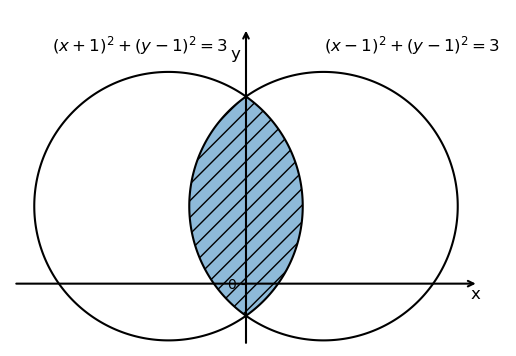
\includegraphics[width=0.9\columnwidth]{Img/cell1.png}
        \bicaption {解空间示意图。} {Solution Space Demo.}
        \label{fig:solution_space}
    \end{figure*}
    
    考虑逻辑公式$F = (x - 1)^2 + (y - 1)^2 \le 3 \wedge (x + 1)^2 + (y - 1)^2 \le 3$,构成的$R^2$空间图形如图\ref{fig:solution_space}所示。两个子句分别表示两个圆的内部,逻辑公式$F$表示同时存在两个圆内部的区域,即图中阴影区域。任何存在于阴影区域内的点都满足逻辑公式$F$,任何满足逻辑公式$F$的点都存在于阴影区域内。因此,解空间$S$是阴影区域的集合。
\label{ex:solution_space}
\end{example}
    
数学上,我们把这样的区域定义为胞腔。

\begin{definition}{\textbf{胞腔}}
对于$R^n$空间上的多项式集合$Q$,$Q$的一个胞腔(cell)是每个多项式$P \in Q$保持符号不变的$R^n$最大联通集合。对于任意的点$a \in R^n$,如果$a$在$Q$的胞腔内,则$a$满足$Q$中的所有多项式,我们记这个胞腔为$cell(Q, a)$。显然,胞腔是$R^n$空间的一个划分。
\end{definition}

对于逻辑公式而言,因为胞腔内的任意一点对每个多项式$P \in Q$保持符号不变,因此SMT公式对应的所有文字仍然保持布尔值不变,不会对SMT公示的满足或不满足造成任何影响。当找到其中任意一个满足逻辑公式的胞腔时,可以判定原公式可满足;当所有胞腔都被证明不可满足时,可以判定原公式不可满足。

给定逻辑公式,如何快速剔除不满足的胞腔并找到可满足的胞腔非常重要,因此现有的研究工作很多聚焦在更好地胞腔划分上。一般的胞腔划分是根据多项式的根和判别式等来判断的,从一个点得到胞腔的划分成为延拓。
\begin{definition}{\textbf{延拓}}
假定$R^n$上的多项式集合$Q$和点$a = (a_1, ..., a_n)$。给定一个变量$x_i (i = 1, 2,..., n)$,假定多项式$
\{q(a_1, ..., a_{i-1}, x_i, a_{i+1}, ..., a_n) | q(a_1, ..., a_{i-1}, x_i, a_{i+1}, ..., a_n) \nequiv 0, q \in Q\}$的实数根$r_1 < r_2 < \cdots < r_s$。一个点$a$关于变量$x_i$在集合$Q$上的延拓定义为一个满足如下性质的点集$\Lambda \subseteq R^n$:
\begin{itemize}
    \item 点$a \in \Lambda$并且对于$1 \leq j \leq s$均存在点$(a_1, ..., a_{i-1}, r_j, a_{i+1}, ..., a_n) \in \Lambda$。
    \item 对于任意点$b = (b_1, ..., b_n) \in \Lambda$,对于$j \in {1, ..., n} \\ {i}$有$b_j = a_j$。
    \item 对于任意的区间$I \in \{(-\infty, r_1), (r_1, r_2), \cdots, (r_{s-1}, r_s), (r_s, +\infty)\}$,都有唯一的$b = (b_1, ..., b_n) \in \Lambda$满足$b_i \in I$。
\end{itemize}
对于点集$\{a^{(1)}, ..., a^{(m)}\} \subseteq R^n$,定义集合关于变量$x_i$在$Q$上的延拓时$\bigcup_{j=1}^m \Lambda_j$,其中$\Lambda_j$是$a^{(j)}$关于变量$x_i$的延拓。
\end{definition}

\begin{example}
\begin{figure*}[]
    \centering
    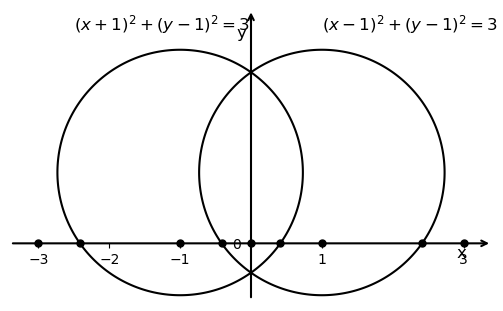
\includegraphics[width=0.45\columnwidth]{Img/cell2.png} \qquad
    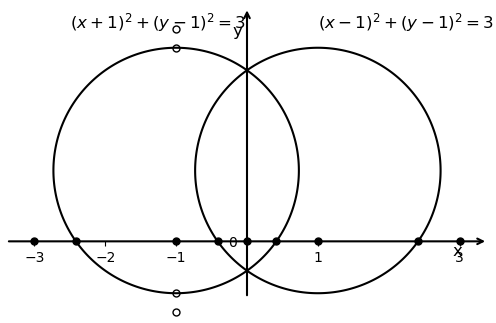
\includegraphics[width=0.45\columnwidth]{Img/cell3.png}
    \bicaption {延拓点集示意图。} {Expansion Demo.}
    \label{fig:expansion}
\end{figure*}
紧接着例子\ref{ex:solution_space},如图\ref{fig:expansion}所示,我们可以得到点$(0, 0)$关于$x$的延拓,即点集$\{(-3, 0), (-1-\sqrt{2}, 0), (-1, 0), (1-\sqrt{2}, 0), (0, 0), (\sqrt{2} - 1, 0), (1, 0), (1+\sqrt{2}, 0), (3, 0)\}$。这些点在$x$变量上分割了多项式的符号区间,从而划分了胞腔在$x$方向上的投影。右侧图的空心点构成了点$(-1, 0)$关于变量$y$的延拓,即点集$\{(-1, -1), (-1, 1-\sqrt{3}), (-1, 1+\sqrt{3}), (-1, 3)\}$,这些点在$y$方向上分开了多项式的符号区间,从而划分了胞腔在$y$方向上的投影。
\label{ex:expansion}
\end{example}
点$a$关于变量$x$的延拓点集事实上是点$a$在方向$x$上相邻胞腔的采样点,如何能够对$R^n$空间上的所有胞腔进行采样是我们接下来的话题。为此,我们引入柱形延拓的概念。

\begin{definition}{\textbf{柱形延拓}}
假设$R^n$上的多项式集合$Q$和点$a$。给定一个变量顺序$x_1 < x_2 < \cdots < x_n$,定义点$a$关于变量顺序在$Q$上的柱形延拓是$\bigcup_{i=1}^n \Lambda_i$,其中$\Lambda_1$是$a$关于变量$x_1$在$Q$上的延拓,并且$\Lambda_{i+1}$是$\Lambda_i$关于变量$x_{i+1}$在$Q$上的延拓。我们把最终的结果$\bigcup_{i=1}^n \Lambda_i$称为$Q$上的柱形延拓。
\end{definition}

柱形延拓可以理解为给定变量顺序下多维的点集延拓,其目的是在$R^n$空间的每一个胞腔上都有一个采样点。
\begin{figure*}[]
    \centering
    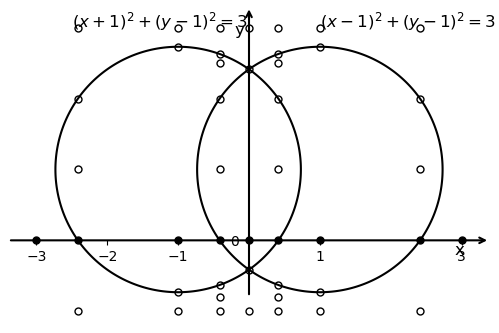
\includegraphics[width=0.9\columnwidth]{Img/cell4.png}
    \bicaption {柱形延拓示意图。} {Cylindrical Expansion Demo.}
    \label{fig:expansion2}
\end{figure*}
\begin{example}
\begin{table*}[]
    % \footnotesize
    \centering
    % \setlength{\tabcolsep}{0.4mm}% column separation
    % \renewcommand{\arraystretch}{1.2}%row space 
    \resizebox{\linewidth}{!}{
        \begin{tabular}{c | c | c | c}
            \hline
            点坐标 & $P_1: (x+1)^2 + (y-1)^2 = 3$根 & $P_2: (x -1)^2 + (y-1)^2 = 3$根 & 根集合\\\hline
            $x \mapsto -3$ & \emptyset & \emptyset & \emptyset \\\hline
            $x \mapsto -1-\sqrt{2}$ & \{0, 2\} & \emptyset & \{0, 2\} \\\hline
            $x \mapsto -1$ & $\{1 - \sqrt{3}, 1 + \sqrt{3}\}$ & \emptyset & $\{1 - \sqrt{3}, 1 + \sqrt{3}\}$ \\\hline
            $x \mapsto 1-\sqrt{2}$ & \{-0.63, 2.63\} & \{0, 2\} & \{-0.63, 0, 2, 2.63\} \\\hline
            $x \mapsto 0$ & $\{1 - \sqrt{2}, 1 + \sqrt{2}\}$ & $\{1 - \sqrt{2}, 1 + \sqrt{2}\}$ & $\{1 - \sqrt{2}, 1 + \sqrt{2}\}$ \\\hline
            $x \mapsto \sqrt{2} - 1$ & \{0, 2\} & \{-0.63, 2.63\} & \{-0.63, 0, 2, 2.63\} \\\hline
            $x \mapsto 1$ & \emptyset & $\{1 - \sqrt{3}, 1 + \sqrt{3}\}$ & $\{1 - \sqrt{3}, 1 + \sqrt{3}\}$ \\\hline
            $x \mapsto 1+\sqrt{2}$ & \emptyset & \{0, 2\} & \{0, 2\} \\\hline
            $x \mapsto 3$ & \emptyset & \emptyset & \emptyset \\\hline
        \end{tabular}
        }
        \bicaption{柱形延拓-区间计算。} {Demo of Computation of Cylindrical Expansion-Interval Splitting.}
\label{tab:expansion}
\end{table*}

\begin{table*}[]
    \tiny
    \centering
    \resizebox{0.65\linewidth}{!}{
        \begin{tabular}{c | c | c}
    \hline
    投影点 & 分割区间 & 延拓点集(采样点)\\\hline
    
    (-3, 0) & $(-\infty, \infty)$ & (-3, 0)\\\hline
    
    \multirow{5}{*}{$(-1-\sqrt{2}, 0)$} & $(-\infty, 0)$ & $(-1-\sqrt{2}, -1)$ \\ & [0, 0] & $(-1-\sqrt{2}, 0)$ \\ & (0, 2) & $(-1-\sqrt{2}, 1)$ \\ & [2, 2] & $(-1-\sqrt{2}, 2)$ \\ & (2, \infty) & $(-1-\sqrt{2}, 3)$ \\\hline
    
    \multirow{5}{*}{(-1, 0)} & $(-\infty, 1-\sqrt{3})$ & (-1, -1) \\
    & $[1-\sqrt{3}, 1-\sqrt{3}]$ & $(-1, 1-\sqrt{3})$ \\
    & $(1-\sqrt{3}, 1+\sqrt{3})$ & (-1, 0) \\
    & $[1+\sqrt{3}, 1+\sqrt{3}]$ & $(-1, 1+\sqrt{3})$ \\
    & $(1+\sqrt{3}, \infty)$ & (-1, 3) \\\hline

    \multirow{9}{*}{$(1-\sqrt{2}, 0)$} & $(-\infty, -0.63)$ & $(1-\sqrt{2}, -1)$ \\
    & [-0.63, -0.63] & $(1-\sqrt{2}, -0.63)$ \\
    & (-0.63, 0) & $(1-\sqrt{2}, -0.5)$ \\
    & [0, 0] & $(1-\sqrt{2}, 0)$ \\
    & (0, 2) & $(1-\sqrt{2}, 1)$ \\
    & [2, 2] & $(1-\sqrt{2}, 2)$ \\
    & (2, 2.63) & $(1-\sqrt{2}, 2.5)$ \\
    & [2.63, 2.63] & $(1-\sqrt{2}, 2.63)$ \\
    & (2.63, \infty) & $(1-\sqrt{2}, 3)$ \\\hline

    \multirow{5}{*}{(0, 0)} & $(-\infty, 1-\sqrt{2})$ & $(0, -1)$ \\
    & $[1-\sqrt{2}, 1-\sqrt{2}]$ & $(0, 1-\sqrt{2})$ \\
    & $(1-\sqrt{2}, 1+\sqrt{2})$ & (0, 0) \\
    & $[1+\sqrt{2}, 1+\sqrt{2}]$ & $(0, 1+\sqrt{2})$ \\
    & $(1+\sqrt{2}, \infty)$ & (0, 3) \\\hline

    \multirow{9}{*}{$(\sqrt{2}-1, 0)$} & $(-\infty, -0.63)$ & $(\sqrt{2}-1, -1)$ \\
    & [-0.63, -0.63] & $(\sqrt{2}-1, -0.63)$ \\
    & (-0.63, 0) & $(\sqrt{2}-1, -0.5)$ \\
    & [0, 0] & $(\sqrt{2}-1, 0)$ \\
    & (0, 2) & $(\sqrt{2}-1, 1)$ \\
    & [2, 2] & $(\sqrt{2}-1, 2)$ \\
    & (2, 2.63) & $(\sqrt{2}-1, 2.5)$ \\
    & [2.63, 2.63] & $(\sqrt{2}-1, 2.63)$ \\
    & (2.63, \infty) & $(\sqrt{2}-1, 3)$ \\\hline

    \multirow{5}{*}{(1, 0)} & $(-\infty, 1-\sqrt{3})$ & $(1, -1)$ \\
    & $[1-\sqrt{3}, 1-\sqrt{3}]$ & $(1, 1-\sqrt{3})$ \\
    & $(1-\sqrt{3}, 1+\sqrt{3})$ & (1, 0) \\
    & $[1+\sqrt{3}, 1+\sqrt{3}]$ & $(1, 1+\sqrt{3})$ \\
    & $(1+\sqrt{3}, \infty)$ & (1, 3) \\\hline

    \multirow{5}{*}{$(1+\sqrt{2}, 0)$} & $(-\infty, 0)$ & $(1+\sqrt{2}, -1)$ \\
    & [0, 0] & $(1+\sqrt{2}, 0)$ \\
    & (0, 2) & $(1+\sqrt{2}, 1)$ \\
    & [2, 2] & $(1+\sqrt{2}, 2)$ \\
    & (2, \infty) & $(1+\sqrt{2}, 3)$ \\\hline

    (3, 0) & $(-\infty, \infty)$ & (3, 0) \\\hline
\end{tabular}
        }
        \bicaption{柱形延拓-采样点生成。} {Demo of Computation of Cylindrical Expansion-Sampling Points.}
\label{tab:expansion2}
\end{table*}

紧接着例子\ref{ex:expansion},如图\ref{fig:expansion2}所示,图中所有的实心点和空心点共同构成了基于变量顺序$x < y$的多项式$Q$的柱形延拓,达到了每个胞腔上均有一个采样点的效果。具体的步骤是,首先点$(0, 0)$关于变量$x$形成延拓(实心点),然后每一个实心点关于变量$y$各自形成延拓(空心点),最终所有点的集合共同构成了柱形延拓。表格\ref{tab:expansion}展示了在实心点处根据多项式集合的根分割得到的区间。表格\ref{tab:expansion2}展示了在每一个分割区间进行采样得到的结果,即最终的柱形延拓点集(空心点)。
\end{example}

\begin{definition}{\textbf{柱形完备}}
对于$R^n$上的多项式集合$Q$,给定一个变量顺序$x_1 < x_2 < \cdots < x_n$,称$Q$对于变量顺序是柱形完备的,当任意的点$a \in R^n$和其关于$Q$的柱形延拓$\Lambda$,$Q$的每一个胞腔都包含至少一个$\Lambda$的点。
\end{definition}
具体的证明请参阅\cite{Caviness2004QuantifierEA,Collins74}。

\subsection{量词消去与柱形代数分解}
根据前文的讨论,我们引出基于多项式解空间的一种量词消去算法-柱形代数分解(Cylindarical Algebraic Decomposition)。

\begin{definition}{\textbf{量词消去}}
量词消去指的是给定一个带有量词的逻辑公式$\varphi$,找到另一个不带有两次的逻辑公式$\psi$,使得$\varphi$和$\psi$的逻辑等价,记为$\varphi \Leftrightarrow \psi$。量词消去的目的是将逻辑公式转化为更易处理的形式,以更好地判断问题的可满足性。
\end{definition}

\begin{example}
考虑多项式$P_s(x, y) = s(x^2 + y^2 - 1) + (1 - s)(xy - 1)$,和逻辑公式$\varphi = \exists R \forall x, y [P_s(x, y) = 0 \Rightarrow x^2 + y^2 \leq R^2]$。量词消去即求解当$s$取什么值的时候逻辑公式$\varphi$满足。通过量词消去工具,我们可以得到$\varphi \Leftrightarrow s \le -1 \wedge s > \frac{1}{3}$。\label{ex:quantifier_elimination}
\end{example}

多项式理论常用的一种量词消去是柱形代数分解(Cylindarical Algebraic Decomposition, CAD)。其核心仍然是把$R^n$空间划分成多个符号一致的胞腔,然后通过判断每个胞腔是否满足逻辑公式进而得到给定变量的赋值区间。如图\ref{fig:CAD}所示,给定变量顺序和多项式集合,柱形代数分解可以分为三个步骤:投影、实根隔离和提升,具体的步骤如下:
\begin{itemize}
    \item \textbf{投影(projection):}从多项式集合开始,每次消去一个变量,生成新的多项式集合,新多项式继续消去变量直到只剩下一个变量为止,记为$proj(P)$。
    \item \textbf{实根隔离(root isolation):}当投影只剩下一个变量时,对当前多项式集合求所有根,得到顺序排列的一组根,这些根表示了胞腔在当前变量上的分割。
    \item \textbf{提升(lift):}提升是对投影阶段得到的多项式集合进行采样。投影从单变量多项式开始,从采样点继续对上一个投影多项式进行采样,直到最终对$R^n$多项式采样,最终保证了每个胞腔得到了采样点。
\end{itemize}

\begin{figure*}[t]
    \centering
    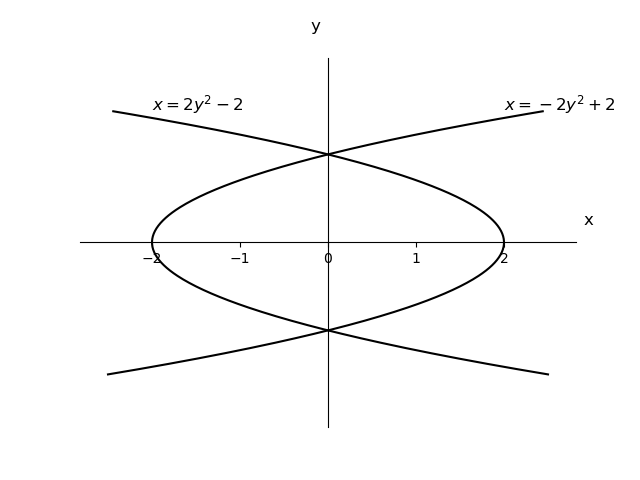
\includegraphics[width=\columnwidth]{Img/cad.png}
    \bicaption {柱形代数分解步骤示意图。} {Demo of Cylindarical Algebraic Decomposition Steps.}
\label{fig:CAD}
\end{figure*}
投影算子(projection operator)指的是投影过程中对多项式集合的计算,比如Collins算子\cite{Collins74}和McCallum算子\cite{McCallum98}。后者因为其计算相对便捷,被广泛应用于量词消去工具和SMT求解器中。

McCallum算子用到的计算包括结式、判别式和求根等操作。
\begin{definition}{\textbf{结式(resultant)}}
对于两个多项式$P_1, P_2 \in R[x_1, ..., x_n]$,假定$$
P_1 = a_m x_n^{d_m} + a_{m-1} x_n^{d_{m-1}} + \cdots + a_0,
$$
$$
P_2 = b_n x_n^{e_n} + b_{n-1} x_n^{e_{n-1}} + \cdots + b_0.
$$
定义$P_1$和$P_2$的结式$Res(P_1, P_2, x_n)$为:
$$
Res(P_1, P_2, x_n) = 
\begin{vmatrix}
    a_m & a_{m-1} & \cdots & a_0 \\
    & a_m & a_{m-1} & \cdots & a_0 \\
    & \ddots & \ddots & \ddots & \ddots & \\
    & & a_m & a_{m-1} & \cdots & a_0 \\

    b_n & b_{n-1} & \cdots & b_0 \\
    & b_n & b_{n-1} & \cdots & b_0 \\
    & \ddots & \ddots & \ddots & \ddots & \\
    & & b_n & b_{n-1} & \cdots & b_0 \\
    \end{vmatrix}
$$
\end{definition}

\begin{definition}{\textbf{判别式(discreminant)}}

对于多项式$P \in R[x_1, ..., x_n]$,假定$$
P = a_m x_n^{d_m} + a_{m-1} x_n^{d_{m-1}} + \cdots + a_0.
$$
定义$P$关于变量$x_n$的判别式$Disc(P, x_n)$为:  
$$
Disc(P, x_n) = \frac{(-1)^{\frac{m(m-1)}{2}}}{a_m} Res(f, \frac{\partial f}{\partial x_n}, x_n). 
$$
\end{definition}

\begin{definition}{\textbf{McCallum投影算子(McCallum Projection Operator)}}

假定$F = \{f_1, f_2, \dots, f_m\}$ 是一组$R^n$上的多项式。McCallum投影算子$proj(F, x_i)$是从$F$到$R^{n-1}$上的多项式集合$proj_m(F)$的一组映射,包含以下元素:
\begin{itemize}
    \item $F$中每个多项式的系数
    \item $F$中每个多项式关于变量$x_n$的判别式
    \item $F$中每两个不同多项式$f_i, f_j$关于变量$x_n$的结式
\end{itemize}
实际计算中,多项式集合的元素通过因式分解化为最简系数的形式,对结果不产生影响。
\end{definition}

\begin{example}
我们给出CAD算法的一个例子。假设$F = \{P_1: x - 2y^2 + 2, P_2: x + 2y^2 - 2\}$,我们规定变量顺序为$y < x$,按步骤计算如下:
\begin{enumerate}
    \item \textbf{投影}:计算对于变量$y$的投影$proj(F, y)$
    \begin{itemize}
        \item 化简后系数多项式为$\{x + 2, x - 2\}$
        \item 化简后判别式为$\{x + 2, x - 2\}$
        \item 化简后结式为$\{x\}$。
    \end{itemize}
    得到投影多项式$proj(F, y) = \{x, x - 2, x + 2\}$

    \item \textbf{实根隔离}:我们对$proj(F, y)$的每个多项式求根,得到根集合$\{-2, 0, 2\}$。
    \item \textbf{提升}:我们对根集合分得的区间进行提升,进一步采样所有胞腔,结果如表格\ref{tab:cad}所示。
    \begin{table*}[]
        \tiny
        \centering
        \resizebox{0.65\linewidth}{!}{
            \begin{tabular}{c | c | c | c | c}
            \hline
            分割区间 & $x$采样点 & $y$根集合 & $(x, y)$采样点 & 符号($P_1, P_2$)\\\hline
            \multirow{5}{*}{$(-\infty, -2)$} & \multirow{5}{*}{$x \rightarrow -3$} & \multirow{5}{*}{$\{-\frac{\sqrt{10}}{2}, \frac{\sqrt{10}}{2}\}$} & (-3, 2) &  (-, +)\\
            & & & $(-3, \frac{\sqrt{10}}{2})$ & (-, 0)\\
            & & & $(-3, 0)$ & (-, -)\\
            & & & $(-3, -\frac{\sqrt{10}}{2})$ & (-, 0)\\
            & & & $(-3, -2)$ & (-, +)\\\hline

            \multirow{7}{*}{$[-2, -2]$} & \multirow{7}{*}{$x \rightarrow -2$} & \multirow{7}{*}{$\{0. -\sqrt{2}, \sqrt{2}\}$} & (-2, 2) &  (-, +)\\
            & & & $(-2, \sqrt{2})$ & (-, 0)\\
            & & & (-2, 1) & (-, -)\\
            & & & (-2, 0) & (0, -)\\
            & & & (-2, -1) & (-, -)\\
            & & & $(-2, -\sqrt{2})$ & (-, 0)\\
            & & & (-2, -2) & (-, +)\\\hline
            \end{tabular}

            To be Done
        }
        \bicaption{柱形代数分解-提升。} {Demo of Cylindrical Algebraic Decomposition - Lift.}
        \label{tab:cad}
    \end{table*}
\end{enumerate}
\label{ex:cad}    
\end{example}

\section{非线性实数理论求解现状}
\subsection{CDCL(T)算法}
CDCL(T) (Conflict Driven Clause Learning for Theories)算法主要是在SAT问题的CDCL搜索框架上增加了理论求解器(Theory Solver),主要的搜索思路包括单元传播、分支决策、冲突分析及回退等CDCL常见技术。理论求解器的作用是对给定的布尔骨架赋值进行推理,当全部布尔骨架得到赋值时通过理论分析返回问题可满足或者报告冲突。具体框架请参见图\ref{fig:cdclt}。

非线性实数的理论求解器主要目的是判断多项式不等式集合的一致性,主要方法可以分为以下几种:
\begin{itemize}
    \item \textbf{区间约束传播(interval constraint propagation, ICP):} 通过变量或者单项式的赋值区间推导出多项式的赋值区间,根据这些区间快速判断一些常见的不一致性。
    \item \textbf{虚拟替代(virtual substitution, VS):} 通过替换多项式中的变量,将多项式转化为更简单的形式,进而判断问题的可满足性。
    \item \textbf{柱形代数分解(cylindrical algebraic decomposition, CAD):} 如前文所述,通过把$R^n$空间划分为多个符号一致的胞腔,逐一排查的方式来推出问题的可满足性。
    \item \textbf{增量线性化(incremental linearization):}把一些多项式线性化,然后使用线性求解器检测问题可满足性,一般是不完备的。
\end{itemize}

\begin{figure*}[t]
    \centering
    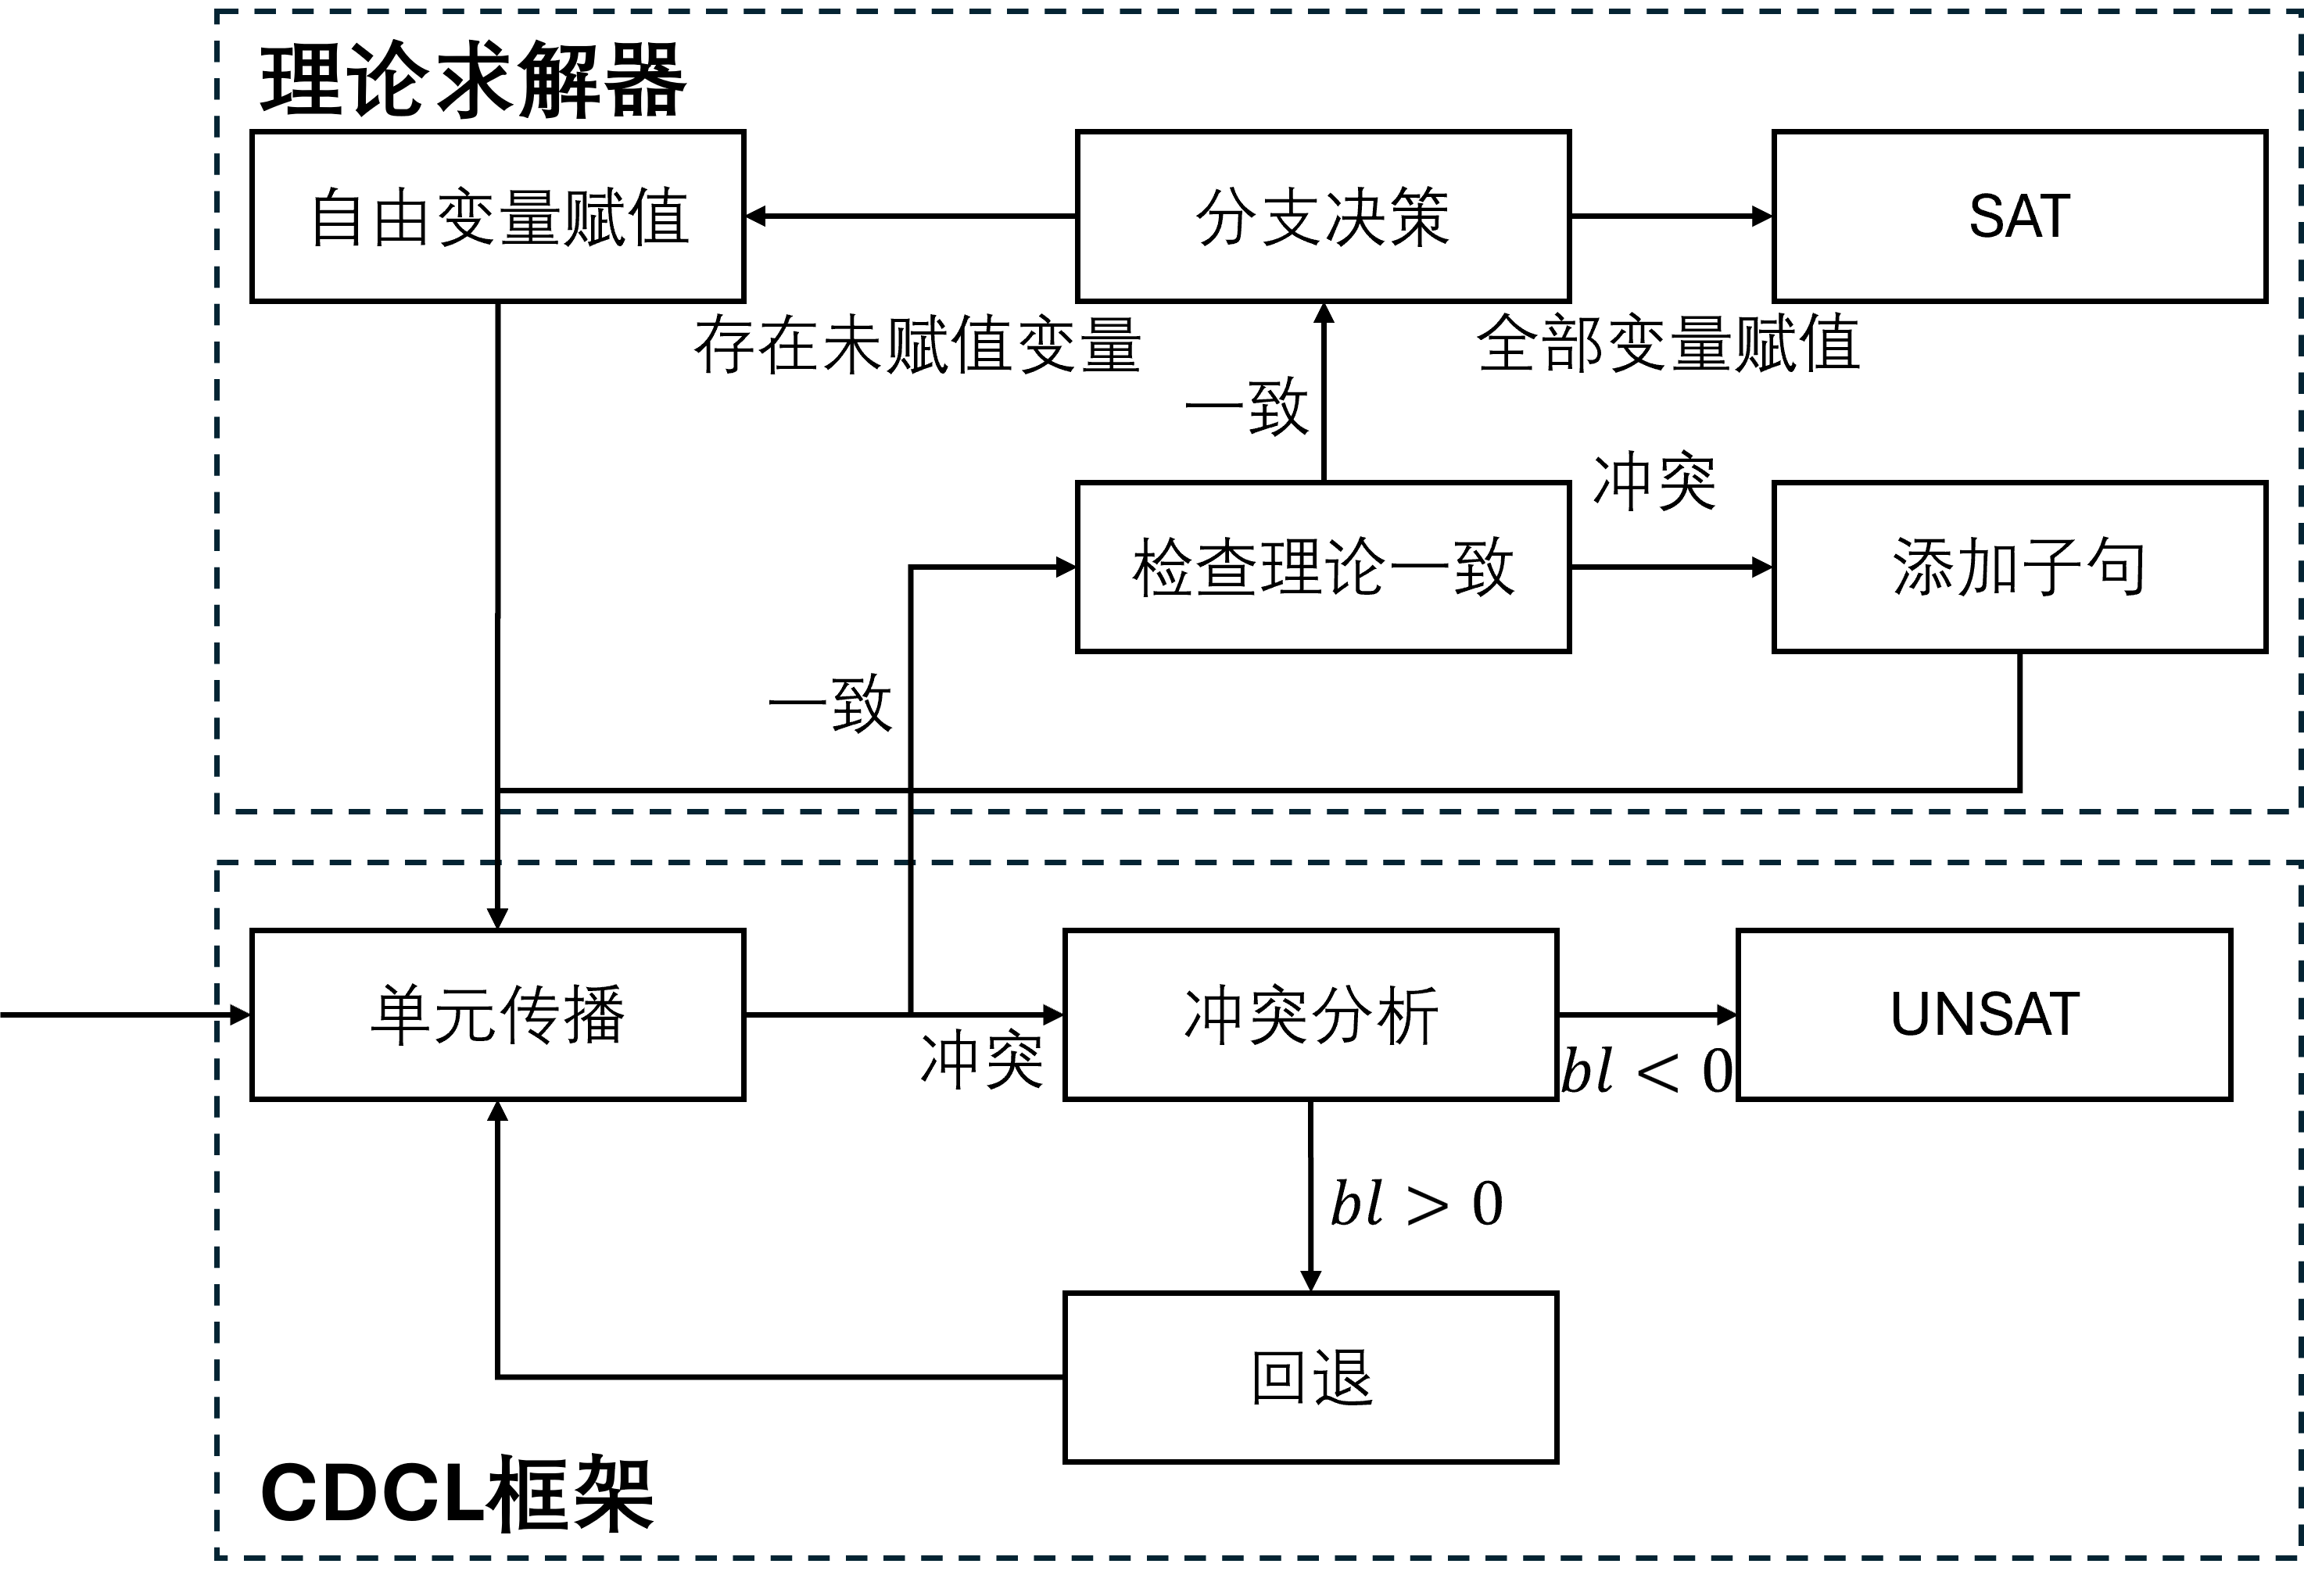
\includegraphics[width=\columnwidth]{Img/cdcl_t.png}
    \bicaption {CDCL(T)框架示意图。} {Demo of CDCL(T) Framework.}
    \label{fig:cdclt}
\end{figure*}

\subsection{MCSAT/NLSAT方法}
MCSAT(Model-Constructing Satisfiability)和NLSAT(NonLinear Satisfiability)是另一种具有CDCL结构的算法,核心的思想仍然是决策赋值、冲突分析和回退。与CDCL(T)不同的是,MCSAT/NLSAT算法加入了基于可行域的算术变量推理,允许在脱离布尔骨架的情况下直接对算术变量进行赋值,一些基本概念介绍如下:
\begin{itemize}
    \item \textbf{决策层数(level):}指文字层面的决策层数,包括布尔文字和算术文字。
    \item \textbf{决策阶段(stage):}指算术变量赋值次数。
    \item \textbf{日志(trace):}一种记录算法更新的线性结构,包括可行域的更新、决策变量的赋值等。
    \item \textbf{算术传播(arithmetic propagation):}基于可行域的文字层面的传播,可以直接推断某些文字的可满足性。
\end{itemize}
其中,MCSAT/NLSAT最关键的步骤就是根据当前变量和文字的可行域关系进行算术文字赋值,假设算术变量的可行域是$curr\_set$,文字的可行域是$lit\_set$,算术传播分为以下几种情况:
\begin{itemize}
    \item \textbf{$lit\_set = \emptyset$:}任何赋值都不能使文字满足,判断文字为$\bot$。比如当$x \mapsto -1$时,文字$y^2 \leq x$不可满足。
    \item \textbf{$lit\_set = R$:}任何赋值都可以使文字满足,直接赋值文字为$\top$。比如文字$x^2 \geq -1$一定满足。
    \item \textbf{$curr\_set \subseteq lit\_set$:}当前文字的可行域包括了算术变量的可行域,因此可以直接判断文字满足。比如当$x \in [-2, 2]$时,文字$x^2 \leq 10$一定满足。
    \item \textbf{$curr\_set \cap lit\_set = \emptyset$:}任何可行域内的赋值都不会让文字满足,因此直接赋值文字为$\bot$。比如当$x \in [-2, 2]$时,文字$x^2 \geq 10$不可满足。
\end{itemize}

例\ref{ex:nlsat}给出了一个MCSAT/NLSAT搜索的具体例子。

\begin{example}
考虑公式$F=(P_1: (x-2)^2 + y^2 \le 4) \wedge (P_2: x - y \ge 0)$。假设我们的搜索顺序是$x < y$,算法的搜索过程如下:
\begin{enumerate}
    \item \textbf{决策算术变量:}赋值$x \mapsto 5$。
    \item \textbf{可行域计算:}计算$P_1$关于变量$y$的可行域是$\emptyset$,发现冲突。
    \item \textbf{冲突分析:}对公式$\exists y. (x-2)^2 + y^2 \le 4$进行量词消去,通过柱形代数分解得到实根$\{0, 4\}$,生成新的学习子句$x \le 4$。
    \item \textbf{回退:}回退到x未赋值的状态。
    \item \textbf{决策算术变量:}重新赋值$x \mapsto 2$。
    \item \textbf{可行域计算:}计算$P_1$关于变量$y$的可行域是$[-2, 2]$,$P_2$关于变量$y$的可行域是$(-\infty, 2]$,取交集得到可行域是$[-2, 2]$。
    \item \textbf{决策算术变量:}赋值$y \mapsto 0$。所有变量得到赋值,返回SAT。
\end{enumerate}
\label{ex:nlsat}
\end{example}

\subsection{局部搜索算法}


\subsection{其他方法}


\section{约束满足问题求解现状}

首先,本文先介绍CSP的定义,它的特点是要求变量的值域有限且离散。前置概念的定义如下。

对于一个变量 $x$,本文用 $D(x)$ 来表示 $x$ 的域,即可以赋予 $x$ 的一组可能的值。通常,使用简写 $x \in \{d_1, \dots, d_m\}$ 来定义 $D(x) = \{d_1, \dots, d_m\}$。特别地,在本文的讨论中仅考虑那些具有有限域的变量。

设 $Y = y_1, y_2, \dots, y_k$ 是一组有限的变量序列,其中 $k > 0$。一个关于 $Y$ 的约束 $c \in C$ 是变量序列 $Y$ 中变量的域的笛卡尔积的子集,即 $c \subseteq D(y_1) \times D(y_2) \times \cdots \times D(y_k)$。约束可以写作 $c(Y)$ 或 $c(y_1, y_2, \dots, y_k)$。如果约束定义在两个变量上,称之为\textit{二元约束}。如果约束定义在两个以上的变量上,称之为\textit{全局约束}。

\begin{definition}[\textbf{约束满足问题}]
    一个CSP,由一组有限的变量序列 $X = x_1, x_2, . . . , x_n$ 及其各自的域 $D = D(x_1), D(x_2), \dots, D(x_n)$ 组成,同时伴有一组约束 $C$,每个约束都在 $X$ 的一个子序列上。为了简化表示,在表示特定的约束集合时经常省略大括号“\{\}”,从而一个CSP被表示为 $P = (X, D, C)$。
\end{definition}

之后,本文给出CSP解的定义。设 $P = (X, D, C)$ 为一个 CSP,其中 $X = x_1, x_2, \dots, x_n$ 且 $D = D(x_1), D(x_2), \dots, D(x_n)$。如果元组 $(d_1, \dots, d_n) \in D(x_1) \times \cdots \times D(x_n)$,并且 $(d_{i_1}, d_{i_2}, \dots, d_{i_m}) \in c$,其中$c \in C$,那么,称关于 $X$ 的这组赋值满足在变量 $x_{i_1}, x_{i_2}, \dots, x_{i_m}$ 上的约束 $C$。

对于变量序列 $K$,定义 $D(K) = \bigcup_{x \in K} D(x)$。当变量 $x$ 的域 $D(x)$ 是单元素集,即 $D(x) = \{d\}$ 时,将其简写为 $x = d$,记作\textit{单域}。

一个CSP是\textit{一致的},如果这个CSP存在解。相反,不存在解的CSP是\textit{不一致的}。一个\textit{失败的}CSP指具有空域(也即存在变量的值域为空)的CSP,或者只有单域的CSP且这些值并不能共同构成CSP的解。一个CSP是\textit{已解决的},若该CSP只有单域,并且其中的赋值可以共同构成CSP的解。需要注意的是,一个失败的CSP也是不一致的,但并非所有不一致的CSP都是失败的。

设 $P = (X, D, C)$ 和 $P' = (X , D', C')$ 都是 CSP。如果 $P$ 和 $P'$ 有相同的解集,那么它们被称为\textit{等价的}。如果 $P$ 和 $P'$ 等价,且对所有的 $x \in X$,都有 $D(x) \subseteq D'(x)$,那么 $P$ 小于 $P'$。这种关系记作 $P \preceq P'$。如果 $P \preceq P'$ 并且至少存在一个 $x \in X$ 使得 $D(x) \subset D'(x)$,那么 $P$ 严格小于 $P'$。这种关系记作 $P \prec P'$。当 $P \preceq P'$ 和 $P' \preceq P$ 都成立时,记作 $P \equiv P'$。

\subsection{约束规划求解}

约束规划的目标是寻找给定的CSP的一个解(或所有解)。求解过程中,值域过滤、约束传播和搜索是交织进行的。

对CSP的解(或所有解)的寻找是通过迭代地将一个CSP分解为更小的CSP来进行的。这个分解过程被称为\textit{构建搜索树}。树的一个节点代表一个CSP。最初,在根节点,得到一个待解决的CSP,记作$P_0$。如果$P_0$既没有被解决也没有失败,就将$P_0$分解为两个或更多的CSP,记作$P_1$,$P_2$,…,$P_k$($k>1$)。同时,必须确保$P_0$的所有解都被保留,而且没有多余的解被添加到$P_0$中。从而,$P_1$,$P_2$,…,$P_k$的解集的并集等于$P_0$的解集。此外,每个CSP $P_i$($i>0$)应该严格小于$P_0$,以确保分解过程能够终止。接下来,会根据上述相同的标准分解每个CSP $P_1$,$P_2$,…,$P_k$。分解会一直进行,直到所有CSP被分解为失败的或已解决的CSP。失败和已解决的CSP是搜索树的叶子节点。

搜索树的大小与$P_0$中变量数量呈指数关系。为了减小搜索树的大小,约束规划使用了一个叫做\textit{约束传播}的过程。给定一个约束$C$,一个\textit{值域过滤算法}会从$C$中的变量的值域中移除与$C$不一致的值。算法必须保留所有的解并且不向$C$中添加任何解。每当一个不一致的值域值被移除,其效果会通过所有其他共享相同对应变量的约束进行传播。这个迭代过程持续进行,直到在CSP中的所有约束都未检测到更多的不一致值。此时,可以称CSP是\textit{局部一致的}。局部一致性反映了算法并没有得到一个全局一致的CSP,而是得到了一个所有约束都是局部的,也即单独的、一致的CSP。这里本文将介绍四个常见的局部一致性:\textit{弧一致性}、\textit{超弧一致性}、\textit{边界一致性}和\textit{区间一致性}。

\begin{definition}[\textbf{弧一致性}]
    一个二元约束$c(x_1, x_2)$是弧一致的,如果对于$x_1$的所有值$d_1 \in D(x_1)$,存在一个值$d_2 \in D(x_2)$使得$(d_1, d_2) \in c$,并且对于$x_2$的所有值$d_2 \in D(x_2)$,存在一个值$d_1 \in D(x_1)$使得$(d_1, d_2) \in c$。
\end{definition}

\begin{definition}[\textbf{超弧一致性}]
    一个约束$c(x_1, ..., x_m)$($m>1$)是超弧一致的,如果对于所有$i \in \{1, ..., m\}$和所有$d_i \in D(x_i)$,存在值$d_j \in D(x_j)$(其中$j \in \{1, ..., m\} - i$),使得$(d_1, ..., d_m) \in c$。
\end{definition}

超弧一致性又称\textit{全局弧一致性}(Generalized Arc Consistency,GAC),相较于弧一致性限制性更强,应用也更广。需要注意的是,弧一致性相当于应用于二元约束的超弧一致性。弧一致性和超弧一致性都确保每个域中的所有值都属于满足约束的元组,与当前变量域相关。另外两种局部一致性概念主要关注变量域的边界。因此,当应用这些定义时,假设涉及的变量域是一个固定的、线性有序的、有限域的元素集的子集。设$D$是这样的一个域,定义$min D$和$max D$分别为其最小值和最大值。此外,使用大括号“\{ \}”和方括号“[ ]”来分别表示一组域值和一个域值区间。

\begin{definition}[\textbf{边界一致性}]
    一个约束$c(x_1, ..., x_m)$($m>1$)是边界一致的,如果对于所有$i \in \{1, ..., m\}$和每个值$d_i \in \{min D(x_i), max D(x_i)\}$,存在值$d_j \in [min D(x_j), \\ max D(x_j)]$(其中$j \in \{1, ..., m\} - i$),使得$(d_1, ..., d_m) \in c$。
\end{definition}

\begin{definition}[\textbf{区间一致性}]
    一个约束$c(x_1, ..., x_m)$($m>1$)是区间一致的,如果对于所有$i \in \{1, ..., m\}$和所有$d_i \in D(x_i)$,存在值$d_j \in [min D(x_j), max D(x_j)]$(其中$j \in \{1, ..., m\} - i$),使得$(d_1, ..., d_m) \in c$。
\end{definition}

在分解一个CSP之后,值域过滤和约束传播被应用到更小的CSP上。值的移除导致搜索树变小,从而加速了解决过程。同时,花费在约束传播上的时间应该小于它引发的加速,以便改善效果显著。关于约束传播过程的详细描述可以在\cite{apt1999essence}和\cite{apt2003principles}中找到,这里不再展开。总之,本文希望应用高效的过滤算法,其效率通常由应用于约束的局部一致性的概念来决定,而在解决过程中何时应用哪种局部一致性的概念则取决于问题本身。

当前主流的求解器分为完备的和启发式的求解器,一些求解器是商用的,而一些则是开源的,他们具有不同的特点,本文介绍三个主流的CP求解器。

\begin{itemize}
% \renewcommand{\labelenumi}{\theenumi)}
    \item Choco。Choco\footnote{\href{https://choco-solver.org/}{https://choco-solver.org/}}是一个基于Java的约束满足问题(CSP)求解库。它提供了一种声明式语言,用于描述和解决各种复杂的约束满足问题。Choco常被用作研究和教学工具,并且支持各种类型的约束,包括数值约束、逻辑约束等。
    \item CPLEX Optimizer。CPLEX Optimizer\footnote{\href{https://www.ibm.com/products/ilog-cplex-optimization-studio}{https://www.ibm.com/products/ilog-cplex-optimization-studio}}是IBM ILOG的一款产品,它包含一个称为CP Optimizer的模块,这是一个约束规划求解器。其主要优点是拥有丰富的API,支持多种编程语言,如C++、Java、Python等,并且它的求解速度非常快,可以处理非常大规模的问题。
    \item Yuck。Yuck是一个基于Scala的运筹学和约束规划库,它的主要特点是它采用了一种基于邻域搜索的算法,可以在解空间中快速找到优质的解。作为一款启发式求解器,他在近几年的CP求解启发式赛道中都是第一名。
\end{itemize}

这些求解器都支持集成在Minizinc\cite{nethercote2007minizinc}中。MiniZinc是一种中间级别的约束建模语言,设计用于描述各种组合优化问题。它的主要目标是提供一种简单、可移植且高效的方式来描述这些问题,以便可以使用各种不同的求解器来解决它们。并且,它支持数组、集合和函数等高级数据结构,以及各种数学和逻辑运算符,并且可以使用CPLEX、Choco、Gecode等求解器作为后端求解器,这使得用户可以在不改变模型的情况下尝试不同的求解器和算法。

\subsection{其他求解方法}

除了CP求解器外,有许多其他的求解技术也可以用来处理CSP,它们来自于不同的研究领域。其中,\textit{布尔可满足性(SAT)求解器}、\textit{可满足性模理论(SMT)求解器}和\textit{整数线性规划(ILP)求解器}是最常用的三种。接下来,本文将介绍这三种求解技术,以及它们在处理CSP时的优势和应用情景。

逻辑公式可满足性问题要求判定一个逻辑公式是否存在使得公式为真的赋值,SAT和SMT问题是其中最主要的两个可满足性问题。SAT问题是第一个被证明为NP完全的问题,是计算机科学的核心问题,也是数理逻辑的基础问题。然而,SAT问题的表达能力和应用范围有其局限性。许多现实问题牵涉到各种领域知识,这就需要用表达能力更强的逻辑公式,比如一阶逻辑公式。尽管一阶逻辑语言是不可判定的,但许多应用只需处理一些背景理论来解释特定的谓词和函数记号的一阶逻辑公式。这类公式被称为SMT公式,它对SAT问题进行了扩展,将其中的布尔变量用背景理论谓词取代。常见的SAT求解器有MiniSAT、Kissat等,而主流的SMT求解器则包含Z3、CVC5等。

\begin{definition}[\textbf{布尔可满足性}]
    一个SAT问题由一系列的布尔变量和逻辑运算符(如与、或、非)构成,对该问题的求解涉及到查找一个给定的布尔公式的满足赋值,使得整个公式的结果为真。
\end{definition}

\begin{definition}[\textbf{可满足性模理论}]
    一个SMT问题可以表示为一个三元组,包含变量集合(可以是整数、实数或者字符串)、函数符号集合(比如常见的运算符、量词等操作)、以及由变量和函数组成的约束集合。
    对该问题的求解涉及到一组变量的赋值,使得约束集合中的约束全部可满足。
\end{definition}

SAT问题是NP完全问题,但现代的SAT求解器已经能够处理数百万个变量和数千万个约束的问题。
将CSP转化为SAT问题的关键步骤是将CSP的变量和约束转化为布尔变量和布尔公式。具体来说,对于CSP中的每一个变量和它的每一个可能的值,都定义一个对应的布尔变量。如果CSP变量被赋予该值,则对应的布尔变量为真;否则为假。然后,可以使用“at most one”和“at least one”的编码方式来保证CSP中的每个变量只能取一个值。同时,CSP的其他约束也可以通过定义相应的布尔公式来实现。

将CSP编码为SMT问题的过程相对直接。由于SMT支持整数变量和约束,以及各种数学函数,因此可以直接将CSP中的变量、约束和函数映射到SMT问题中。
这样,CSP就可以被转化为一个等价的SAT/SMT问题,进而利用相应求解器求解。一般来言,在编码CSP时,SAT的编码复杂度要高很多,但比涉及高阶逻辑的SMT求解器拥有更好的性能。

最后是ILP,它是线性规划(LP)的一种扩展。线性规划问题包含一组线性约束条件和一个线性目标函数,问题的目标是在满足这些约束条件的前提下,找到使目标函数取得最大(或最小)值的变量的取值,而ILP则要求所有的决策变量都是整数。
由于CSP中的变量通常也是整数,因此CSP可以很自然地映射为ILP问题。常见的ILP求解器有Gurobi、SCIP等。

这些算法为解决CSP提供了新的视角,尽管某些转换可能相对复杂,可能会影响性能或效率,但它们也弥补了CP求解器在特定问题时的不足。

\section{AllDifferent约束求解现状}

由于目前AllDifferent约束的过滤算法及后续算法都要用到图论的相关知识,所以本文先介绍图论以及相关的最大匹配算法,之后介绍AllDifferent约束的过滤算法以及基于该算法的一些改进策略。

\subsection{图论基础}

本文用$G = (V, E)$表示一个(无向)图,其中$V$是一个有限的顶点集,而$E$是来自$V$的无序对的多重集,称为边。顶点$u \in V$和$v \in V$之间的边记作$uv$。
如果存在一个分区$S, T$,使得$E \subseteq \{st | s \in S, t \in T \}$,那么图$G = (V, E)$称为\textit{二部图},写作$G = (S, T, E)$。

在图$G = (V, E)$中,\textit{游走}指一个序列$P = v_0, e_1, v_1, \dots, e_k, v_k$,其中$k \geq 0$,$v_0, v_1, \dots, v_k \in V$,$e_1, e_2, \dots, e_k \in E$,并且对于$i = 1, \dots, k$,有$e_i = v_{i-1}v_i$。如果$v_0, \dots, v_k$是不同的,那么这个游走就被称为一条\textit{路径}。一个闭合的路径,即$v_0 = v_k$,称为\textit{回路}。

图$G = (V, E)$的子图是一个图$G' = (V', E')$,它满足$V' \subseteq V$和$E' \subseteq \{uv | u \in V', v \in V', uv \in E\}$。称子图$G' = (V', E')$为图$G = (V, E)$的\textit{最大连通子图},若对于$V'$中的每一对$u, v$,在$G'$中都存在一条$u$到$v$的路径。

有向图是一个对$G = (V, A)$,其中$V$是一个有限的顶点集,$A$是来自$V$的有序对的多重集,称为弧,从$u \in V$到$v \in V$的弧记作$(u, v)$。
类似于无向二部图,如果存在一个分区$S, T$,使得$A \subseteq \{(s, t) | s \in S, t \in T \}$,那么有向图$G = (V, A)$就是二部图。也写作$G = (S, T, A)$。
此外,关于有向图的路径、回路、子图、最大连通子图等概念和无向图类似,这里不再展开。

在有向图中,如果存在两个顶点$s$和$t$,从$s$可以通过一条有向路径到达$t$,同时也可以从$t$通过一条有向路径到达$s$,那么就说两个顶点\textit{相互到达}。如果在一个有向图中,存在一个顶点集$V$,对于集合中的任意两个顶点$u$和$v$都可以相互到达,称$V$为\textit{强连通分量}(Strongly Connected Component,SCC)。

图$G = (V, E)$的一个\textit{匹配}指一组不相交的边集$M \subseteq E$,即$M$中的任意两条边不共享顶点。如果$M$包含了所有属于$S \subseteq V$的顶点,称匹配$M$覆盖了$S$。如果$M$没有覆盖顶点$v \in V$,那么$v$就被称为$M$-free,又称自由节点;如果$M$覆盖了顶点$v \in V$,称$v$为匹配节点。
匹配$M$的大小是$|M|$,若最大匹配包含了图中所有的顶点,那么这个匹配被称为\textit{完全匹配}。

\begin{definition}[\textbf{最大图匹配}]
    给定一个无向图$G = (V, E)$,其中$V$是顶点集,$E$是边集。最大图匹配问题要求找出图中一个最大的匹配。
\end{definition}

设$M$是图$G = (V, E)$中的一个匹配。如果一条路径$P$的长度是奇数,它的两端没有被$M$覆盖,并且它的边交替出现在$M$的外部和内部,那么称$P$为\textit{$M$-增广路径}。如果回路$P$的边交替出现在$M$的外部和内部,那么称$P$为\textit{$M$-交替路径}。
在$M$-增广路径上,可以交换在$M$中和不在$M$中的边,得到的$M'$仍然是一个匹配,并且其中的$|M'| = |M| + 1$。因此可以得到如下的定理,证明如下。

\begin{proof}
如果$M'$是一个比$M$大的匹配,考虑图$G' = (V, M \cup M')$。在$G'$中,每个顶点最多连接两条边。因此,$G'$的每个组件要么是一个回路,要么是一条路径(可能长度为零)。由于$|M'| > |M|$,因此至少有一个组件包含的$M'$的边比$M$的边多。因为所有的回路都包含偶数条边,所以这个组件必须是一个$M$增广路径。如果$M'$是一个比$M$大的匹配,考虑图$G' = (V, M \cup M')$。在$G'$中,每个顶点最多连接两条边。因此,$G'$的每个组件要么是一个回路,要么是一条路径(可能长度为零)。由于$|M'| > |M|$,因此至少有一个组件包含的$M'$的边比$M$的边多。因为所有的回路都包含偶数条边,所以这个组件必须是一个$M$增广路径。
\end{proof}

\begin{theorem}
   设$G = (V, E)$是一个图,$M$是$G$中的一个匹配。那么$M$要么是最大匹配,要么存在一个$M$-增广路径。
\end{theorem}

因此,可以通过在$G$中迭代计算$M$-增广路径并扩展$M$的方式来求一个图最大匹配,它是求解最大图匹配的一类经典方法,步骤如下。

设$G = (U, W, E)$是一个二部图,$M$是$G$的一个匹配。通过将$M$中的所有边从$W$指向$U$,并将所有其他边从$U$指向$W$,构造有向二部图$G_M = (U, W, A)$,即:
\begin{equation*}
    A = \{(w, u) | uw \in M, u \in U, w \in W \} \cup \{(u, w) | uw \in E \setminus M, u \in U, w \in W \}
\end{equation*}

然后,在$G_M$中从$U$中的一个自由顶点开始并在$W$中的一个自由顶点结束的每一条有向路径对应于$G$中的一个$M$-增广路径。通过选择$|U| \leq |W|$,最多需要找到$|U|$条这样的路径。由于每条路径可以通过广度优先搜索在最多$O(|A|)$时间内被识别,因此这个算法的时间复杂度是$O(|U||A|)$。

在\cite{hopcroft1973n}中提出了其改进算法,可以在$O(|V|^{1/2}|A|)$时间内运行,其中$V = U \cup W$。其思想为,与其反复沿着单个$M$-增广路径增强$M$,不如反复同时沿着一组不相交的$M$-增广路径增强$M$。这样的路径集合可以再次在$O(|A|)$时间内找到。可以证明,在$|V|^{1/2}$次迭代之后,通过对路径长度的推理,最多可能还有$O(|V|^{1/2})$次迭代,这导致总的时间复杂度为$O(|V|^{1/2}|A|)$。而在一个普通的图$G = (V, E)$(不一定是二部图)中,可以在$O(|V||E|)$时间内\cite{edmonds1965paths}或者$O(|V|^{1/2}|E|)$时间内\cite{micali1980v}计算出最大的匹配。

\subsection{AllDifferent约束和二部图匹配}

本文首先展示AllDifferent约束的解和二部图中的匹配的等价性。为此,本文将AllDifferent约束涉及的变量使用二部图进行表示,称为\textit{值图}。它的定义如下,注意,定理中的匹配$M$覆盖了$X$,因此是最大匹配。此外,本文给出了一个例子来描述这一转换过程。
\begin{definition}[\textbf{值图}]
设$X$是一组变量集合,则二部图$G = (X, D(X), E)$,其中$E = \{xd | d \in D(x), x \in X\}$,被称为$X$的值图。
\end{definition}

\begin{theorem}
设$X = x_1, x_2, \dots, x_n$是一系列变量,$G$是$X$的值图。那么$(d_1, \dots, d_n) \in \texttt {AllDifferent}(x_1, \dots, x_n)$当且仅当$M = \{x_1d_1, \dots, x_nd_n\}$是$G$中的一个匹配。
\end{theorem}

\begin{proof}
在$M$中的边$x_id_i$(对于某个$i \in \{1, . . . , n\}$)对应于赋值$x_i = d_i$。由于$M$中的边不共享顶点,所以对于所有$i \neq j$,都有$x_i \neq x_j$。
\end{proof}

\begin{figure*}[t]
    \centering
    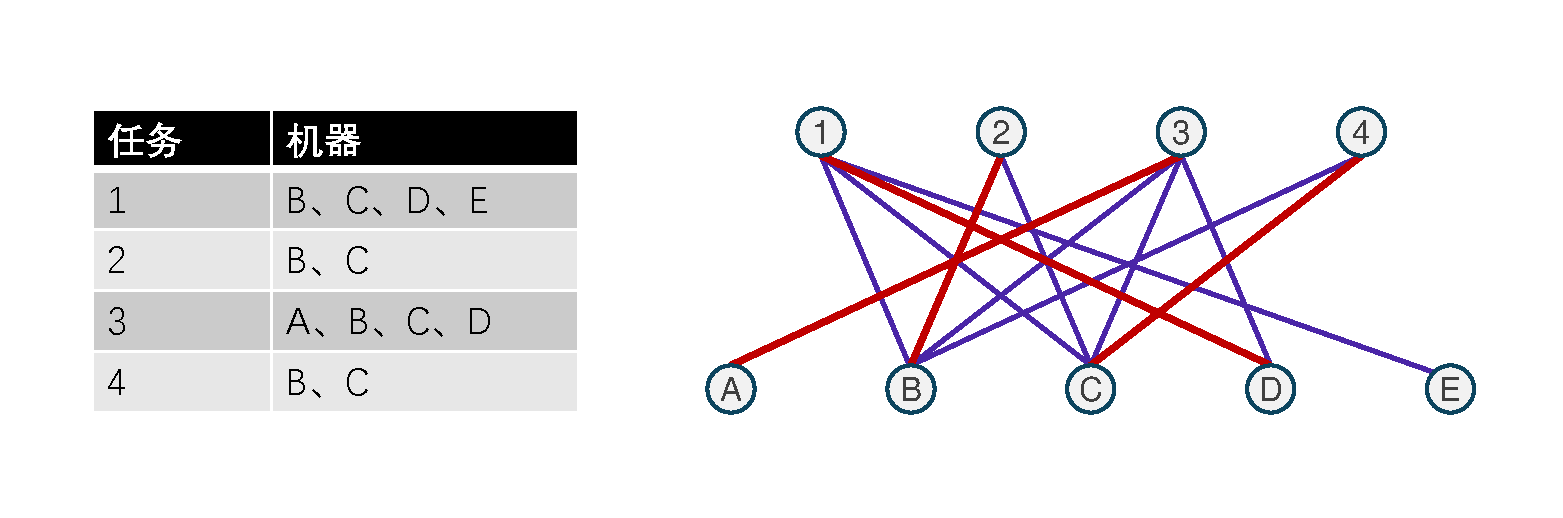
\includegraphics[width=\columnwidth]{Img/A&G.pdf}
    \bicaption {AllDifferent约束和其二部图表示。} {AllDifferent constraint and its bipartite graph representation.}
    \label{fig:AandG}
\end{figure*}

\begin{example}
    假设有四个任务(1,2,3和4)要被分配给五台机器(A,B,C,D和E)。每台机器最多只能分配一个任务,但并非每个任务都能分配给每台机器。图\ref{fig:AandG}左中展示了可能的组合,例如,任务2可以分配给机器B和C。
    由于任务必须分配给不同的机器,可以使用AllDifferent约束表述该问题,从而将问题建模为CSP。具体地,引入一个变量$x_i$,用于表示任务$i = 1, \dots, 4$,其赋值代表任务$i$被分配到的机器。变量的初始值域为图\ref{fig:AandG}左表示的任务和机器之间可能的组合,下式是构造的CSP约束:
    \begin{equation*}
        \texttt {AllDifferent}(x_1, x_2, x_3, x_4).
    \end{equation*}
    其中,$x_1 \in \{B, C, D, E\}, x2 \in \{B, C\}, x_3 \in \{A, B, C, D\}, x_4 \in \{B, C\}$。
    设$X = x_1, \dots, x_n$,其值图如图\ref{fig:AandG}右所示。值图中的红粗线表示覆盖$X$的一个匹配,它对应于CSP的解,即$x_1 = D, x_2 = B, x_3 = A$和$x_4 = C$。
\end{example}

最后,本文要介绍Hall的婚配定理\cite{hall1987representatives},它是用于推导AllDifferent约束过滤算法的图论中的一个经典定理,旨在描述一个二部图存在完全匹配的必要和充分条件。
这个定理的直观解释是,如果每个女孩(A集合)都有足够多的男孩(B集合)可以选择,那么就有可能为每个女孩找到一个男孩作为配对,形成一个完全匹配,反之亦然。
接下来,本文给出AllDifferent约束语境下,该定理的形式化描述,证明略。

\begin{theorem}\label{theorem:Hall}
    约束条件$\texttt {AllDifferent}(x_1, \dots, x_n)$有解,当且仅当对于所有的$K \subseteq \{x_1, \dots, x_n\}$,下式成立:
    \begin{equation*}
        |K| \leq |D(K)|
    \end{equation*}
    
\end{theorem}

\begin{example}
    考虑如下CSP:
    \begin{equation*}
        \texttt {AllDifferent}(x_1, x_2, x_3, x_4).
    \end{equation*}
    其中,$x_1 \in \{2, 3\}, x_2 \in \{2, 3\}, x_3 \in \{1, 2, 3\}, x_4 \in \{1, 2, 3\}$。
    可见,对于任何$K \subseteq \{x_1, x_2, x_3, x_4\}$且$|K| \leq 3$,都有$|K| \leq |D(K)|$。然而,对于$K = \{x_1, x_2, x_3, x_4\}$,有$|K| > |D(K)|$。由定理\ref{theorem:Hall}可知,这个CSP没有解。
\end{example}

\subsection{AllDifferent约束的过滤算法}

前面,本文介绍了局部一致性的概念,本文以弧一致性为例介绍AllDifferent约束如何应用局部一致性,本文首先利用二元分解将AllDifferent约束分解成一组二元约束,其定义如下。

\begin{definition}[二元分解]
设C是变量$x_1, \dots, x_n$上的一个约束。C的二元分解指在$x_1, \dots, x_n$的变量对上的一组最小的二元约束$C_{dec} = \{C_1, \dots, C_k\}$(其中$k$为整数且$k > 0$),使得C的解集等于$\bigcap_{i=1}^{k} C_i$的解集。
\end{definition}

关于$\texttt {AllDifferent}(x_1, x_2, \dots, x_n)$的二元分解是
\begin{equation}
    \bigcup_{1 \leq i < j \leq n} \{xi \neq xj\}.
\end{equation}
建立二元分解上的弧一致性的过滤算法很简单:每当一个变量的域只包含一个值时,这个值就从在AllDifferent约束中出现的其他变量的值域中被移除。这个过程一直重复,直到没有更多的变化发生或者一个域变为空。通过这个算法,可以建立AllDifferent约束上的局部一致性,或者证明它是不一致的。换句话说,当一个值域包含多个元素时,就不能推理出更多的信息了。

这个算法的一个缺点是,需要$\frac{1}{2}(n^2 - n)$个不等约束来表示一个n元的AllDifferent约束,从而这种方法的最坏情况时间复杂度是$O(n^2)$。另一个更重要的缺点是信息的丢失。当二元约束集合被弧一致化时,一次只比较两个变量。而当AllDifferent约束被超弧一致化时,所有的变量都被同时考虑,这允许更强的局部一致性,下面本文给出一个简单的例子。

\begin{example}
设一个CSP包含三个变量$x_1, x_2, x_3$,其中$x_1 \in \{2, 3\}, x_2 \in \{2, 3\}, x_3 \in \{1, 2, 3\}$。对于约束$\texttt {AllDifferent}(x_1, x_2, \dots, x_n)$,在不采用二元分解时,通过超弧一致性,可以删减$x_3$值域中的2和3;而对该AllDifferent约束使用二元分解时,由于约束被分解为多个二元约束,此时无法推导出任何信息。
\end{example}

前面,提到了AllDifferent约束和二部图的等价性,以及求解二部图最大匹配的方法。接下来,本文介绍一种利用二部图实现的GAC算法,它基于最大匹配和强连通分量,称为\textit{Régin算法}\cite{regin1994filtering}。算法思路是构造残差图表示AllDifferent约束,并通过在图上作图匹配删减冗余边,实现在约束上的全局一致性。

后文需要用到前面定义的CSP的一些概念,为了方便后文叙述,本文额外引入几个新定义。
约束$c$的\textit{变量集}是它所限制的有序变量集,记作$X(c) = \{x_1, x_2, \dots, x_r\}$。$c$的\textit{值域}是$X(c)$的值域的并集,记作$D(c) = \bigcup_{x \in X(c)} D(x)$。此外,本文使用$B_c(a)$来表示$X(c)$中值域包含$a$的变量集(即,$B_c(a) = \{x | x \in X(c), a \in D(x)\}$)。
在AllDifferent约束表示的二部图中,\textit{冗余边}指在任何最大匹配中都不出现的边。\textit{允许边}则表示属于一些但不一定所有最大匹配的边,冗余边和允许边是互补的。

一个节点是允许的,当且仅当对于一个任意的最大匹配$M$,它可以通过一个从自由节点开始的偶数交替路径到达。交替路径中的变量节点集被记为$\Gamma$,其值节点集被记为$A$。
关于允许边有如下定理,证明略。

\begin{theorem}
    一个AllDifferent约束是GAC的,当且仅当它的值图的每个边都是允许边,也即属于在$B(c)$中覆盖$X(c)$的一些匹配。
\end{theorem}

\begin{theorem}[\textbf{Berge定理}]
    一个边是允许的,当且仅当,对于一个任意的最大匹配$M$,它属于从自由节点开始的偶数增广路径或者偶数交替路径。
\end{theorem}

基于上述定理,Régin提出了执行GAC的第一个AllDifferent约束算法,通过从值图中移除冗余边来实现GAC。
该算法首先计算一组AllDifferent约束的值图的最大匹配,通过引入新的节点和将边改为有向边,构造\textit{残差有向图}如下。

\begin{definition}[\textbf{残差有向图}]
    残余有向图被定义为$R = \langle V_R, E_R \rangle$,其中$V_R = X(c) \cup D(c) \cup \{t\}$,$t$是与$D(c)$连接的一个新引入的汇节点,$E_R = E_M \cup E_U \cup E_{t_1} \cup E_{t_2}$。具体来说,每个边$e \in E_M \cup E_U$表示约束$c$中的一个变量-值对。匹配边$E_M$将变量连接到它们各自的匹配值:$E_M = \{x \rightarrow a | x \in X(c), a = M(x)\}$。未匹配的边$E_U$将值连接到它们各自的未匹配变量:$E_U = \{a \rightarrow x | a \in D(c), x \in B_c(a) \setminus \{M (a)\}\}$。$E_{t_1}$中的边将匹配值节点连接到$t$:$E_{t_1} = \{a \rightarrow t | M (a) \in X(c)\}$。$E_{t_2}$中的边将$t$连接到未匹配的值节点(自由节点):$E_{t_2} = \{t \rightarrow a | M (a) \notin X(c)\}$。
\end{definition}

通过残差有向图,可以发现,通过引入汇节点$t$,从自由节点开始的偶数增广路径被扩展为偶数的交替路径,从而允许边表现为残差图上的交替路径。
此外,很容易发现,交替路径上的顶点之间的其他边也可以扩展成一个交替路径,因此也属于允许边。从而得到如下定理:
\begin{theorem}
    一个非匹配边是允许的,当且仅当其顶点处于同一个强连通分量中。
\end{theorem}
因此,算法会计算残差有向图的强连通分量(SCC),这是算法最耗时的部分,通常通过Tarjan算法来解决。之后会删除两个端点处于不同强连通分量的非匹配边。图\ref{fig:Residual}展示了一个简单的值图转换为残差图的例子,在右图中每个框表示一个SCC,而紫红色的线段就是应当被删除的冗余边。

\begin{figure*}[t]
    \centering
    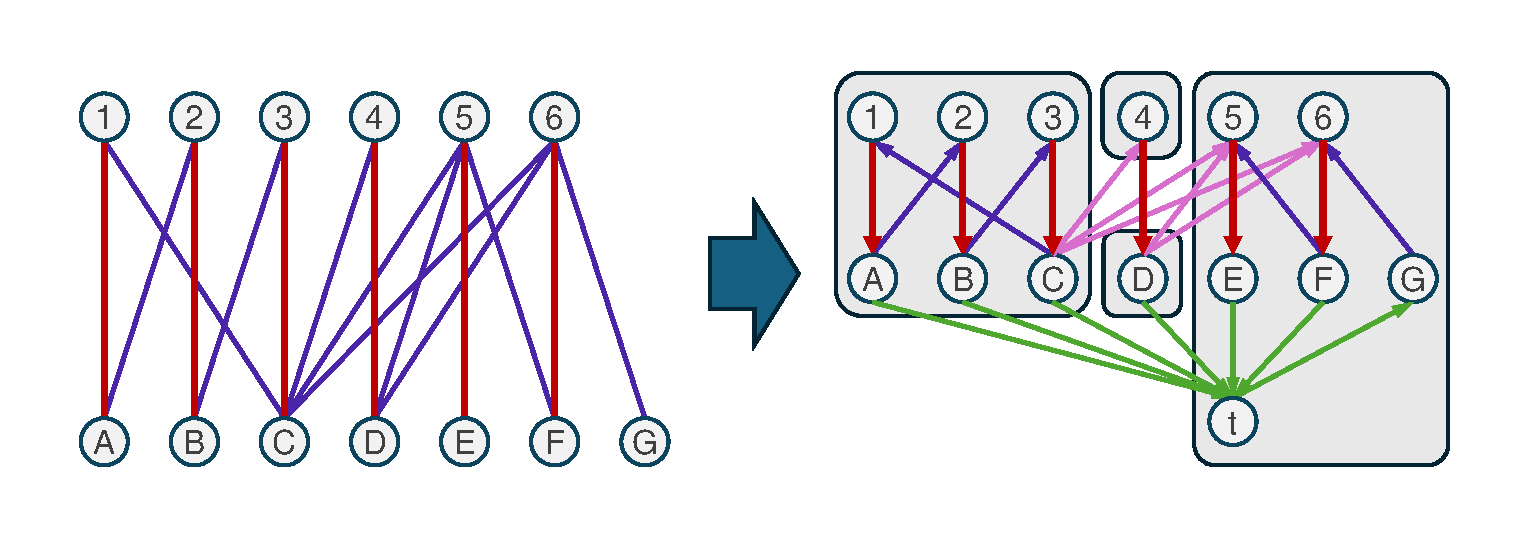
\includegraphics[width=\columnwidth]{Img/Residual.pdf}
    \bicaption {值图与残差有向图的转换。} {Value graph to residual directed graph transformation.}
    \label{fig:Residual}
\end{figure*}

近几年,有许多基于该算法的改进工作,主要思路是减少或避免SCC的计算。例如:SCC-分割\cite{gent2008generalised},它只计算在回溯搜索过程中其变量的域已经改变的SCC,从而减少了计算SCCs所需的变量范围;
匹配优化\cite{zhang2018fast},它证明了冗余边可以分为两类,其中一类可以直接删除,无需计算相应的SCCs;
早期检测\cite{zhang2021early},它避免了计算那些删除后不会分割当前SCCs的无关紧要的边;
在文献\cite{li2023bitwise}中,证明了二部图中的所有冗余边都指向某些交错环,从而对值进行筛选;
在文献\cite{zhen2023eliminating}中,发现GAC算法只关心图模型的一个节点是否在SCC中,而不是它属于哪个SCC,从而使用比特位提高算法的性能。

\section{局部搜索算法现状}

局部搜索是相对于完备搜索来说的,它是一种用于解决优化问题的常用启发式策略,而几乎所有问题都可以看作是一类优化问题,例如组合优化问题。
局部搜索的基本思想是从一个初始状态开始,然后在解的邻域中寻找更好的状态,通过一系列的移动来改进当前解。一些基本的概念的定义如下。

\begin{definition}[\textbf{状态}] 状态是解空间中的一个元素,表示问题的一个可能解。\end{definition}

\begin{definition}[\textbf{移动}] 移动是从当前状态转移到邻域中的另一个状态的操作。 \end{definition}

\begin{definition}[\textbf{打分函数}] 打分函数(评价函数)是一个将解空间中的每个状态映射到实数的函数,用于评估每个状态的优劣,即解的质量。 \end{definition}

\begin{definition}[\textbf{邻域}] 邻域是一个状态执行一次移动后的所有可达状态的集合。\end{definition}

% \begin{example}
%     设有一个旅行销售员问题,包含四个城市A、B、C和D。一个可能的状态(路径)是ABCD。如果我们交换B和C的顺序,我们就进行了一个移动,并得到一个新状态ACBD。这个状态就是原状态的邻域中的一个元素。 
% \end{example}

为了实施局部搜索算法,首先需要明确候选解的邻域结构,即确定哪些候选解可以被视为邻居。一旦邻域结构被定义,问题的解空间就可以被视为一个图形结构。因此,局部搜索实际是在图论问题上求解。以下是其求解流程:
\begin{enumerate}
    \item 设 $S = \{s_1, s_2, \ldots, s_n\}$ 为所有候选解构成的解空间,也即状态空间。
    \item 定义初始状态 $s_0 \in S$,一般由构造的初始化函数得到。
    \item 定义邻域函数 $N : S \rightarrow \mathcal{P}(S)$,将每个状态映射到其邻域的状态集合。
    \item 定义目标函数 $f : S \rightarrow \mathbb{R}$,用于评估每个状态的好坏,即解的质量。
    \item 设置停止条件,当满足某个特定条件时终止算法。常见的停止条件如达到最大迭代次数、最大时间限制等。
    \item 由打分函数(可能多个)构成移动规则,指导从当前状态的邻域中选择下一个状态。一般选择使得目标函数变好最多的状态。
    \item 从初始状态 $s_0$ 开始,按照移动规则在邻域中选择下一个状态,更新当前状态。重复这个过程,直到达到最优解或满足其他停止条件。
\end{enumerate}

若将被满足的约束数量作为最小化目标,则CSP可以被看作组合优化问题,通过局部搜索,寻找使得CSP中一致约束最多的赋值。本文以一个简单的CSP为例,介绍上面提到的概念和算法流程。

\begin{example}
假设有一个简单的约束满足问题(CSP),其中有三个变量 $X = \{x_1, x_2, x_3\}$,每个变量的取值范围是 $\{1, 2, 3\}$。目标是找到一组赋值 $A = \{a_1, a_2, a_3\}$,使得所有的约束 $C = \{c_1, c_2, c_3\}$ 都被满足。在这个问题中,状态就是变量的一组赋值,比如 $s = \{2, 1, 3\}$。移动就是改变一个变量的赋值,比如从状态 $\{2, 1, 3\}$ 移动到状态 $\{2, 2, 3\}$。目标函数就是被满足的约束数量,本文希望最小化未被满足的约束数量,也就是最大化被满足的约束数量。邻域就是通过一次移动可以达到的所有状态,比如从状态 $\{2, 1, 3\}$ 可以移动到的状态有 $\{1, 1, 3\}$、$\{3, 1, 3\}$、$\{2, 2, 3\}$、$\{2, 3, 3\}$、$\{2, 1, 1\}$和$\{2, 1, 2\}$。此时从一个初始赋值开始,通过移动来最小化未满足约束的数量,直到得到可满足解。
\end{example}

近几年,局部搜索算法发展出了很多策略,这些策略可以根据问题的特性和需求进行组合,以提高局部搜索算法的效率和效果。下面是一些例子:
\begin{itemize}
    \item \textbf{禁忌搜索\cite{glover1990tabu}}:这种策略旨在避免在已经访问过的区域中陷入循环。在禁忌搜索中,会维护一个禁忌表,记录一些在近期内已经访问过的状态。当从当前状态的邻域中选择下一个状态时,禁忌表中的状态将被排除在外。
    \item \textbf{重启策略}:重启策略能够有效避免搜索过程陷入局部最优解。若如果搜索过程在一段时间内没有找到更好的解,算法会随机选择一个初始状态重新开始搜索。这样可以使搜索过程有机会探索解空间的其他区域。 
    \item \textbf{迭代局部搜索\cite{lourencco2003iterated}}:这种策略在没有达到局部最优时,持续执行迭代改进算法。当达到局部最优时,执行随机游走算法,即从当前的局部最优解出发,进行一次或多次随机的移动,以跳出当前的局部最优区域。策略的目标是搜索一系列的局部最优解,然后返回最好的一个作为结果。
    \item \textbf{解池技术}:解池技术在搜索过程中不仅保存当前最优解,还保存一些具有代表性的非最优解,这些解构成了一个解池。通常他和重启策略一起使用,在重启时,算法从解池中选择一个解执行随机游走后得到初始状态,重新开始搜索。
\end{itemize}

在近十年来,已经有不少工作采用局部搜索来对CSP问题进行求解,并帮助解决了许多此前未解决的难题,下面本文列举一些经典及最新的工作。

在文献\cite{codognet2001yet}中,作者设计了一种新的启发式算法,它利用了问题在约束和变量方面的结构,可以比全局代价函数更精确地指导搜索进行优化(例如,违反约束的数量)。
该工作在拉丁方、N皇后、全间隔等问题上进行了实验,并且取得了较好的实验结果。
在文献\cite{DBLP:journals/tec/JinH19}中,作者设计了将拉丁方问题转化为图的方法,从而将问题归约到图着色问题上,并使用遗传算法,对给定补全拉丁方实例进行求解,取得了较好的求解效率。
在文献\cite{lloyd2020antcolony}中,作者设计了针对数独问题的蚁群算法,并尝试了多种邻域的定义,算法可以在25x25阶的困难数独实例上取得高达95\%的求解成功率。
在文献\cite{pan2022fast}中,作者设计了针对性的解池技术和子代价函数,并通过高效的化简规则对CSP进行了化简,其在拉丁方问题上,可以求解绝大部分70阶的拉丁方补全问题。


\section{本章小结}

本章节介绍了CSP、AllDifferent约束的形式化定义以及主流的求解它们的算法。
在第一节中,本文介绍了CSP的求解现状,主要介绍了CP求解器,以及其他可用于求解的技术,如SAT、SMT、ILP求解器等。
在第二节中,本文介绍了ALlDifferent约束的求解现状,主要介绍了它和图匹配的关系,以及两种主流的针对该约束的过滤算法。
在第三节中,本文介绍了局部搜索算法的概念和求解流程,以及相关的各类技术。
\chapter{基于可行域的胞腔跳跃缓存机制}\label{chap:method1}
本章首先总结了前述工作的胞腔跳跃算法,并通过例子给出当前算法带来的操作冗余性。接着,本章给出一种更合理的基于变量可行域的胞腔跳跃操作,并且针对每次迭代中可行域的重复计算问题给出数据结构的形式化表示。具体而言,本章引入边界(boundary)的概念来刻画几何上胞腔之间的界限,从而可以进一步计算变量不同赋值对分数的影响。最后,本章介绍了算法迭代中边界的实时迭代算法,具体表现为当邻居变量发生移动后,所在子句的所有算术变量需要重新计算边界,其余子句的边界不受影响。最后,本文给出局部搜索算法LS\_NRA中操作选择与执行部分,并通过例子详细展示一个SMT约束如何通过计算和更新边界来进行迭代求解。

\section{胞腔跳跃操作(Cell-Jump Operation)}
变量的操作移动是局部搜索算法的核心概念,即每一步如何更改变量的赋值,以期望在搜索空间中找到更好的解。在布尔可满足问题(SAT问题)中,变量的操作被定义为翻转(Flip),即将变量的赋值从真($\top$)改为假($\bot$)或反之。SMT问题因为其赋值的多样性(整数或实数)使得变量的移动操作更为复杂。一个经典的操作是关键移动(critical move)\cite{CaiLZ22},即使得文字不等式恰好达到满足状态时对应的整数赋值操作。工作\cite{multilinear}将关键移动拓展到了实数操作上,即允许变量赋值为实数。对于多项式理论的关键移动,工作\cite{LiXZ23}借助胞腔的概念首次提出胞腔跳跃操作(Cell-Jump),具体定义如下:

\begin{definition}{\textbf{平行坐标轴的胞腔跳跃(Cell-Jump Parallel to Axis)}}\\
假设当前赋值为$\alpha = \{x_1 \mapsto a_1, x_2 \mapsto a_2, \cdots, x_n \mapsto a_n\}$。$l$是赋值$\alpha$下未满足的多项式不等式,假定其不等式符号为<或者>。
\begin{itemize}
    \item 假定$l$具有形式$p(x) < 0$。对于每一个单变量多项式$p(a_1, \cdots, a_{i-1}, x_i, a_{i+1}, \cdots, a_n)$具有负值采样点的变量$x_i$来说,存在一个胞腔跳跃操作,记为$cjump(c_i, l)$,即赋值$x_i$到离$a_i$最近的负值采样点。
    \item 假定$l$具有形式$p(x) > 0$。对于每一个单变量多项式$p(a_1, \cdots, a_{i-1}, x_i, a_{i+1}, \cdots, a_n)$具有正值采样点的变量$x_i$来说,存在一个胞腔跳跃操作,记为$cjump(c_i, l)$,即赋值$x_i$到离$a_i$最近的正值采样点。
\end{itemize}
如果把赋值看作是$R^n$空间中的一个点,那么前面的胞腔跳跃操作就是沿着平行坐标轴的直线$(a_1, \cdots, a_{i-1}, R, a_{i+1}, \cdots, a_n)$移动到另一个点。
\end{definition}

\begin{definition}{\textbf{沿着固定直线的胞腔跳跃(Cell-Jump Along Fixed Straight Line)}}\\
    假设当前赋值为$\alpha = \{x_1 \mapsto a_1, x_2 \mapsto a_2, \cdots, x_n \mapsto a_n\}$。$l$是赋值$\alpha$下未满足的多项式不等式,假定其具有形式$p(x) > 0$或$p(x) < 0$。给定一个方向向量$dir = (d_1, \cdots, d_n)$。引入新变量$t$,对于多项式$p(x)$中的每一个变量$x_i$,用$a_i + d_i t$来替换得到新的多项式$p^{*}(t)$。如果$l$不等式符号为<并且多项式$p^{*}(t)$具有负值采样点,那么定义胞腔跳跃操作$cjump(dir, l)$为将赋值$\alpha$沿着方向$dir$移动到离原点最近的负值采样点。如果$l$不等式符号为>并且多项式$p^{*}(t)$具有正值采样点,那么定义胞腔跳跃操作$cjump(dir, l)$为将赋值$\alpha$沿着方向$dir$移动到离原点最近的正值采样点。假设采样点为$t^*$,则更改后的赋值为$\alpha' = \{x_1 \mapsto a_1 + d_1 t^*, \cdots, x_n \mapsto a_n + d_n t^*\}$。
\end{definition}

\begin{figure*}[t]
    \centering
    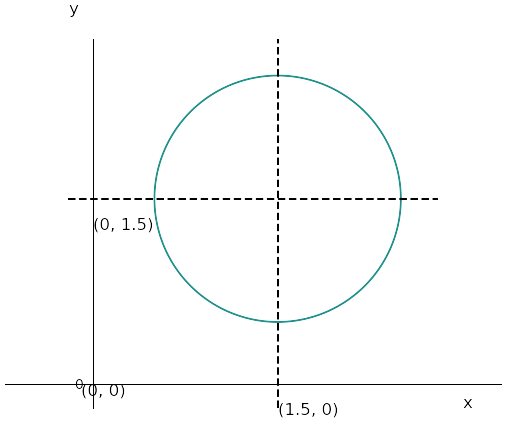
\includegraphics[width=0.45\columnwidth]{Img/jump1.png}\qquad
    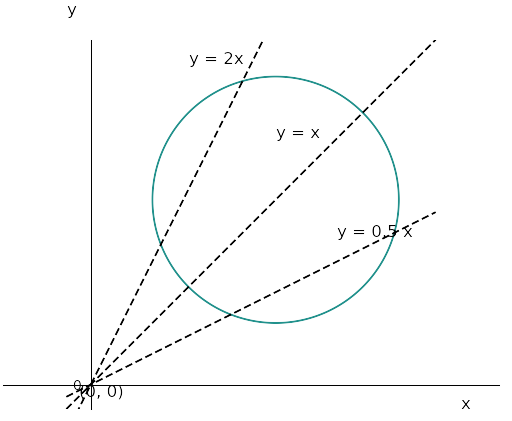
\includegraphics[width=0.45\columnwidth]{Img/jump2.png}
    \bicaption {胞腔跳跃操作示意图。} {Demo of cell-jump operations.}
\label{fig:cell-jump}
\end{figure*}

\begin{example}
如图\ref{fig:cell-jump}所示,给定公式$F = \{(x - 1.5)^2 + (y - 1.5)^2 < 1\}$,赋值$\alpha_1 = \{x \mapsto 1.5, y \mapsto 0\}, \alpha_2 = \{x \mapsto 0, y \mapsto 1.5\}, \alpha_3 = \{x \mapsto 0, y \mapsto 0\}$。$F$在赋值$\alpha_1, \alpha_2, \alpha_3$下均不满足。

如左图所示,当局部搜索算法选择初始赋值为$\alpha_1$时,通过平行y轴的胞腔跳跃可以得到操作$y \mapsto 1.5$使得不等式满足;同理当初始赋值为$\alpha_2$时,通过平行x轴的胞腔跳跃可以得到操作$x \mapsto 1.5$使得不等式满足。当局部搜索算法选择初始赋值为$\alpha_3$时,任何平行坐标轴的移动都不会使不等式满足,因此算法存在停滞的风险。

右图表示了基于固定直线的胞腔跳跃操作,定义三组方向向量分别为$dir_1 = \{1, 2\}, dir_2 = \{1, 1\}, dir_3 = \{2, 1\}$,对应的胞腔跳跃操作分别为$cjump(F, dir_1)$, $cjump(F, dir_2)$, $cjump(F, dir_3)$,替换后的多项式和可行域(保留三位小数)分别为:
\begin{align*}
    F_1 &= \{(t - 1.5)^2 + (2t - 1.5)^2 < 1\} \rightarrow (0.568, 1.232), \\
    F_2 &= \{(t - 1.5)^2 + (t - 1.5)^2 < 1\} \rightarrow (0.793, 2.207), \\
    F_3 &= \{(2t - 1.5)^2 + (t - 1.5)^2 < 1\} \rightarrow (0.568, 1.232).
\end{align*}
三个多项式的可行域均不为空,因此可以选取合适的值$t$同时移动变量$x$和$y$使得约束满足。
\end{example}

\section{基于变量级别可行域的操作缓存机制}
前述工作的胞腔跳跃操作都是基于单一子句进行的,通过收集所有不满足子句的操作最终决定最优的操作进行执行。但是,在实际的局部搜索迭代中,一个变量可能同时出现在多个子句中,因此在每次迭代中都需要重复计算变量的可行域。除此之外,基于单一子句的胞腔操作容易造成操作的冗余,从而减慢整体迭代效率。我们以例\ref{ex:jump}进行说明。

\begin{example}
\label{ex:jump}
考虑逻辑公式$F = \{P_1: (x-1)^2 + (y-1)^2 \leq 3, P_2: (x+1)^2 + (y-1)^2 \leq 3\}$,假设当前赋值为$\alpha: \{x \mapsto -1.5, y \mapsto 0.5\}$。可知当前赋值仅满足$P_1$,不满足$P_2$。我们考虑平行于x轴的胞腔跳跃操作$cjump(P_1, x)$,即图\ref{fig:jump2}中虚线所示。

\begin{figure*}[t]
    \centering
    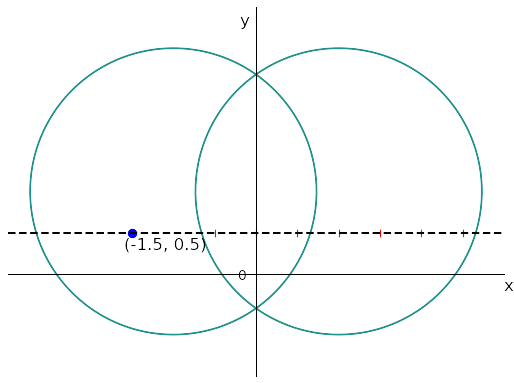
\includegraphics[width=0.45\columnwidth]{Img/op1.png}\qquad
    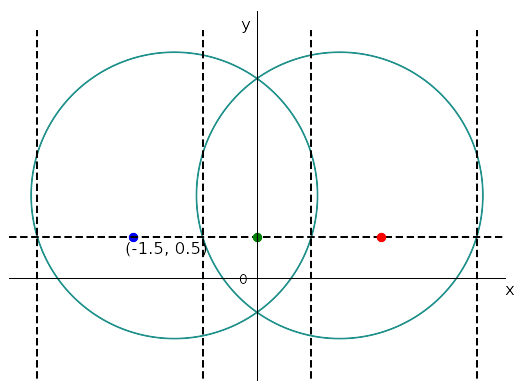
\includegraphics[width=0.45\columnwidth]{Img/op2.png}
    \bicaption {基于变量级别可行域的胞腔跳跃操作。} {Cell-jump operation based on variable-level feasible-set.}
\label{fig:jump2}
\end{figure*}

\textbf{传统计算方法(图\ref{fig:jump2}左图):}
\begin{itemize}
    \item 我们首先计算变量$x$对约束$P_1$的可行域$(-0.658, 2.658)$。
    \item 根据可行域我们进行采样,比如选取7个采样点得到$\{-0.5, 0, 0.5, 1, 1.5, 2, 2.5\}$,如图\ref{fig:jump2}左图中短竖线所示。
    \item 我们对这5个采样点逐一计算分数,选取其中分数最大的操作,比如$\{x \mapsto 0\}$。
    \item 移动后的赋值$\{x \mapsto 0, y \mapsto 0.5\}$满足约束$P_1$和$P_2$,找到可行解,算法停止。
\end{itemize}

这种方法带来了两个潜在的问题:
\begin{enumerate}
    \item 因为目前的胞腔跳跃操作$cjump(P_1, x)$是基于单一约束设计的,因此选择的采样点有可能同时破坏当前已经满足的约束。虽然我们可以通过打分函数进行筛选,但更好的方式是选择操作的时候进行简单判断。图\ref{fig:jump2}左图中,红色采样点表示破坏了原先$P_2$的可满足状态,而绿色采样点表示保持了$P_2$的可满足状态。
    \item 在每次迭代中,我们只会根据当前约束的可行域进行采样,因此可能造成整体$R^n$空间上同类操作的冗余,从而在接下来的打分函数计算环节降低了算法的效率。比如在图\ref{fig:jump2}左图中,红色竖线同属一个胞腔,绿色竖线同属另一个胞腔,同一个胞腔对SMT公式的影响完全相同,没必要重复计算。
\end{enumerate}

\begin{definition}{\textbf{同类操作(Similar Operations)}}
    对于多项式约束$P$,给定两个胞腔跳跃操作$cjump_1(P, x)$和$cjump_2(P, x)$,他们分别将变量$x$移动到不同的赋值。如果两个移动后的赋值$\alpha_1$和$\alpha_2$在解空间上存在于同一个胞腔中,我们定义两个操作是同类操作,记作$cjump_1(P, x) \sim cjump_2(P, x)$。
\end{definition}
从图中可以看出,更好地刻画胞腔跳跃操作需要引入变量在多个子句的可行域概念,综合所有可行域后才能可以得到可行域-分数的对应关系。我们把改进的计算方法描述如下:

\textbf{改进计算方法(图\ref{fig:jump2}右图):}
\begin{itemize}
    \item 首先计算变量$x$对两个约束$P_1$和$P_2$各自的可行域: $(-0.658, 2.658)$和$(-2.658, 0.658)$。
    \item 综合两个可行域,我们可以得到$R$上的一个划分:$(-2.658, -0.658)$, $(-0.658, 0.658)$, $(0.658, 2.658)$。
    \item 对于每一个部分,我们只需要选择一个采样点即可,然后计算当前操作的得分,选择分数最佳的操作。如图\ref{fig:jump2}右图中,我们选择了红色$(0, 0.5)$和绿色$(1.5, 0.5)$两个采样点,前者同时满足两个约束,而后者仅仅满足$P_1$约束。
    \item 检查移动后的赋值$\alpha: \{x \mapsto 0, y \mapsto 0.5\}$,找到可行解,算法停止。
\end{itemize}
比较两种算法,可以看出传统算法采样在单一子句可行域计算时进行,也仅仅维护了赋值-分数的对应关系;而改进后的算法通过综合多个子句的可行域,维护了$R$上每一个赋值和分数的映射关系,可以非常方便计算出对应的操作分数。除此之外,因为传统算法提前采样的特点,产生了大量的冗余操作,改进后的算法因为直接在胞腔层面进行了维护,因此采样点的选择更具有合理性。
\end{example}

我们把$R$上胞腔的分割定义为\textbf{边界(boundary)},具体定义如下:
\begin{definition}{\textbf{边界(boundary)}}
我们定义\textbf{边界(boundary)}为一种四元组数据结构$<val, is\_open, is\_make, cid>$,其中$val$是实数,表示边界的值,$is\_open$是布尔值,表示边界是否为开区间,$is\_make$是布尔值,表示边界处分数递增还是递减,$cid$表示该处边界对应的子句编号。我们定义边界之间的排序为:首先$val$值小的排在前面,如果$val$相同,$is\_open$为假的排在前面,这样我们可以得到一组按照实数自然排序的边界集合(boundary set)。
\end{definition}
需要注意的是,边界仅仅刻画变量从边界左侧移动到边界右侧对应的约束变化情况(可满足到不可满足,不可满足到可满足),如果要计算对应胞腔的具体分数,需要从边界处采样点进行计算。我们使用例\ref{ex:jump2}进行说明。

\begin{example}
\label{ex:jump2}
\begin{figure*}[t]
    \centering
    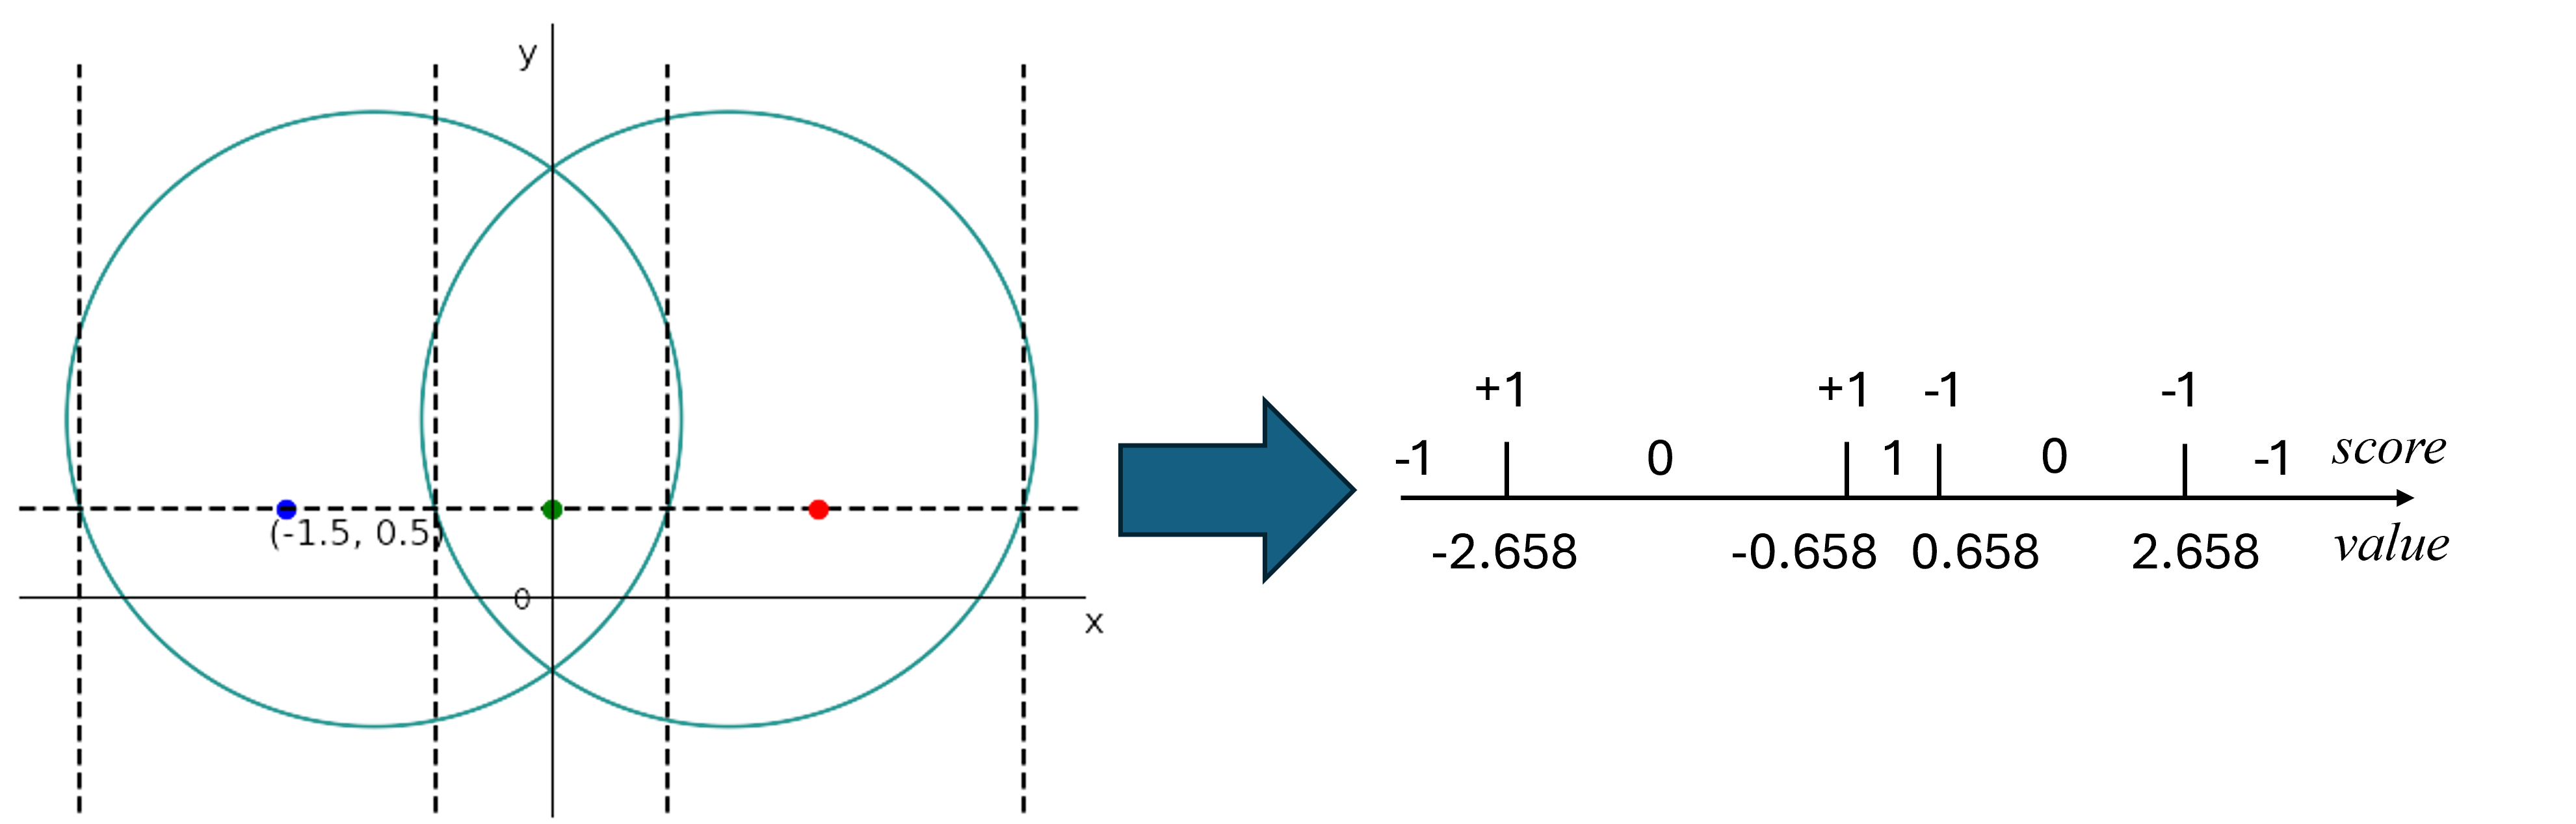
\includegraphics[width=\columnwidth]{Img/boundary.png}
    \bicaption {边界计算示意图。} {Demo of Coomputation of Boundaries.}
\label{fig:boundary}
\end{figure*}

仍然考虑例\ref{ex:jump}中的约束和赋值,约束$P_1$和$P_2$的可行域是:$(-0.658, 2.658)$和$(-2.658, 0.658)$。在边界处,变量从左向右移动会导致相应约束的满足状态发生变化,假设每个约束的权重为1,可以计算得到$R$上的四个边界如下:
\begin{align}
Boundary_1 &: <-2.658, \top, \top, 2> \nonumber \\
Boundary_2 &: <-0.658, \top, \top, 1> \nonumber \\
Boundary_3 &: <0.658, \bot, \bot, 1> \nonumber \\
Boundary_4 &: <2.658, \bot, \bot, 2> \nonumber
\end{align}
四次边界处的分数变化均为1。为了求得赋值和分数的对应关系,我们需要在每个分割的胞腔处采样,然后计算分数。一种更简单的办法是计算某一个胞腔处的分数,然后根据边界的分数变化计算其他胞腔处的分数。可以注意到,当变量$x$移动到和原来赋值所在的胞腔时(比如例子中的$(-2.658, -0.658)$),对应的分数一定为0。为了计算的方便性,我们引入\textbf{起始分数(starting score)}的概念来表示数轴最左侧代表的分数。

\begin{definition}{\textbf{起始分数(Starting Score)}}
我们定义起始分数为一个实数值,表示数轴上最左侧点对应的分数,即变量移动到$-\infty$时对应的分数。
\end{definition}
在本例子中,最左侧的赋值会破坏原先已经满足的$P_2$约束,因此分数为-1。在每次边界处我们增加或减少对应的分数,因此可以得到图\ref{fig:boundary}右侧的结果。边界和分数的计算展示在算法\ref{alg:score}中。
\end{example}

\begin{algorithm}[t]
    % \small
    \caption{Computation of best critical move and score}
    \label{alg:score}
    \textbf{输入}: variable $x$, boundary set $B$ and starting score $s_0$\\
    \textbf{输出}: Best critical move range $val$ and score $score$
    \begin{algorithmic}[1] %[1] enables line numbers
        \Statex \hrulefill

        \State $score \leftarrow -\infty$;
        \State $s \leftarrow s_0$;
        \FOR{each boundary $b$ in $B$}
            \STATE $s \leftarrow s + s_{change}$;
            \IF{$s > score$}
                \STATE $score \leftarrow s$;
                \STATE $val \leftarrow b.val$;
            \ENDIF
        \ENDFOR
        \RETURN $val$ and $score$
    \end{algorithmic}
\end{algorithm}

在局部搜索算法中,每一次迭代只会改变一个变量的赋值,因此绝大多数约束的可满足状态和可行域不会发生变化,一个可行的优化是增量式计算变量的边界集合。具体而言,当一个变量的赋值发生改变时,只有其所在的约束会发生相应的赋值变化,只有那些约束所包含的变量的边界需要更新。为方便说明,我们定义邻居变量的概念如下:

\begin{definition}{\textbf{邻居变量(Neighbor Variables)}}
    对于变量$x$,其所在的约束集合记为$C_x$,那么$x$的邻居变量集合$N_x$定义为$N_x = \{y | \exists c \in C_x, y \in Var(c) \land y \neq x\}$。
\end{definition}

\begin{algorithm}[t]
    % \small
    \caption{Incremental computation of make-break move and scores}
    \label{alg:update}
    \textbf{输入}: Variable $v$ that is modified\\
    \textbf{更新}: Make-break move and scores
    \begin{algorithmic}[1] %[1] enables line numbers
        \Statex \hrulefill

        \State $V \leftarrow \emptyset$;
        \FOR{each clause $cls$ that contains $v$}
            \FOR{variable $v'$ in $cls$}
                \STATE $V \leftarrow V \cup \{v\}'$;
                \STATE boundary $bd \leftarrow $ compute boundary of $v'$ with respect to  $cls$;
                \STATE add $bd$ to boundary set $S_{v'}$;   
            \ENDFOR
        \ENDFOR

        \FOR{variable $v'$ in $V$}
            \STATE recompute best critical move and score for $v'$; \Comment{algorithm \ref{alg:score}}
        \ENDFOR
    \end{algorithmic}
\end{algorithm}

在具体实现中,我们的算法为每一个变量维护一个边界集合$S_vx$,当一次迭代带来变量$v$赋值发生变化后,我们重新计算其包含的每个约束$c$对邻居变量$v'$的新边界,然后更新到其边界集合$S_{v'}$中。在所有边界更新完毕后,我们对每个邻居变量$v'$重新计算其最佳的边界和分数,以方便下一次算法迭代。算法\ref{alg:update}展示了伪代码。

下面的例子\ref{ex:update}展示了边界计算的更新过程。

\begin{example}
\label{ex:update}
考虑约束集合$F = \{P_1: x^2 + y^2 \leq 1, P_2: x + y < 1, P_3: x + z > 0\}$。当前赋值为$\alpha: \{x \mapsto 1, y \mapsto 1, z \mapsto 1\}$,所有约束权重为1。则当前状态每个约束关于变量$x$的可行域和边界计算如下:
\begin{align}
& x^2 + y^2 \leq 1  \rightarrow x \in [0, 0] \nonumber & \quad \text{Boundary: } & \{<0, \bot, \top, 1>, <0, \top, \bot, 1>\} \nonumber \\
& x + y < 1  \rightarrow x \in (-\infty, 0) \nonumber & \quad \text{Boundary: } & \{<0, \bot, \bot, 1>\} \nonumber \\
& x + z > 1  \rightarrow x \in (-1, +\infty) \nonumber & \quad \text{Boundary: } & \{<-1, \top, \top, 1>\} \nonumber
\end{align}
排序后的边界集合为:
$$
\{<-1, \top, \top, 1>, , <0, \bot, \top, 1>, <0, \top, \bot, 1>, <0, \bot, \bot, 1>\}
$$

当某次迭代发生赋值$y \mapsto -2$时,约束$x + y < 1$有不满足状态变为可满足状态。由于变量$y$和$z$不为邻居变量(没有共同存在的约束),因此我们无需更改变量$z$的边界。对于前两个同时存在变量$x$和$y$的子句,我们需要重新计算关于变量$x$的边界信息。

\begin{align}
& x^2 + y^2 \leq 1  \rightarrow x \in \emptyset \nonumber & \quad \text{Boundary: } & \emptyset \nonumber \\
& x + y < 1  \rightarrow x \in (-\infty, 3) \nonumber & \quad \text{Boundary: } & \{<3, \bot, \bot, 1>\} \nonumber
\end{align}
排序后的边界集合为:
$$
\{<-1, \top, \top, 1>, <3, \bot, \bot, 1>\}
$$
\end{example}

除了本章节提到的设计之外,边界信息的维护仍然存在以下几种优化空间:
\begin{itemize}
    \item \textbf{更复杂的数据结构:}除了使用边界(线性数据结构)维护变量赋值-分数关系之外,也可以使用二叉树等顺序存储的数据结构。一般来说,当变量的边界个数很小时(SMT-LIB中大多数样例),现行的数据结构已经足够高效。对于更多操作,二叉搜索树也许更为高效。
    \item \textbf{迭代优化:}在每次迭代中,由于我们只会从未满足子句中选择操作,因此我们可以只更新那些出现在未满足子句中的变量的边界信息,而不是所有的邻居变量。除此之外,我们可以使用更懒惰的办法,比如为特定需要更新的约束打标记,然后在其不可满足时才更新边界信息。
\end{itemize}

\section{本章小结}
本章节首先回顾了以往工作提出的用于求解算术SMT问题的胞腔跳跃操作,具体包括平行坐标轴和沿固定直线两种方法。然后,本文根据一个例子指出了以往针对单个子句的胞腔操作存在冗余问题,并且在迭代过程中容易造成可行域缓存的损失,基于此本文给出了边界和同类操作的定义以及操作缓存机制。最后,本工作给出了邻居变量的定义,并借此给出可行域缓存机制的迭代条件,即只有邻居变量的赋值发生变化时才需要更新边界信息。本工作还讨论了可能的优化,比如更复杂的数据结构或者更新条件等。
\chapter{等式松弛机制}\label{chap:method2}

本章节主要介绍局部搜索算法在LS\_NRA处理等式约束时的松弛技术,主要可以分为两个阶段:松弛阶段和恢复阶段。
首先,本章节考虑到局部搜索迭代算法的效率问题,引入赋值复杂度的概念,并提出非线性实数理论独有的无理数赋值挑战。
紧接着,本文提出一种等式松弛方法来暂时扩大约束的可行域,从而保证了有理数赋值,使得算法可以找到附近的近似解。
然后,本文探讨了算法最后的恢复阶段,即近似解如何恢复为原问题的精确解,并提出了具体的懒惰版本的实现方法。
最后,本文介绍了其他的一些可行的改进策略。

\section{代数数赋值的复杂度}
在SMT问题的四种主流算术理论(线性整数理论、线性实数理论、非线性整数理论、非线性实数理论)中,非线性实数理论(NRA)因为其存在高次多项式约束与潜在的无理数赋值问题而最难处理。这些情况基本发生在等式约束上,例如$x^2 + y^2 = 2$等。对于局部搜索迭代而言,尽管在计算机中可以使用代数数表示无理数,但无理数赋值问题带来的仍是多项式评估的效率低下,进而影响到实根隔离与计算可行域等操作。除此之外,一些分母较大的代数数仍然会影响计算速度。

以往的工作\cite{multilinear,LiXZ23}都尽量避免了代数数引发的计算问题,因此将非线性问题限定为多线性约束(multilinear)或至少包含一个线性项的等式约束上。其中,工作\cite{multilinear}考虑了有理数赋值的分母大小问题,并将其作为操作得分相同时的打破平均策略。

我的工作考虑了非线性实数的全部测试样例,一个关键的优化是尽量减少复杂赋值的出现频率。为此,我首先定义赋值之间的复杂度关系如下:

\begin{definition}{\textbf{赋值复杂度(Complexity of values)}}
\label{def:complexity}
我定义代数数上的偏序$\prec_c$如下。$x \prec_c y$当且仅当以下任何一种情况成立:

\begin{itemize}
    \item $x$和$y$都是有理数,且$x$的分母小于$y$的分母。
    \item $x$是有理数,而$y$是无理数。
\end{itemize}
当$x \prec_c y$或者$y \prec_c x$均不成立时,我认为$x$和$y$的复杂度相当,记为$x \sim_c y$。
\end{definition}

\section{松弛机制}
我将等式的松弛机制简单描述如下:每次当等式或者不等式约束迫使某一个变量必须赋值为一个相对复杂的代数数时,我会暂时松弛这些约束,使用复杂度相对低的松弛解,然后以松弛的形式继续局部搜索的迭代过程。在具体实现上,我引入以下两个参数来设置算法门槛:
\begin{itemize}
    \item $\epsilon_v$:根据定义\ref{def:complexity}衡量表示代数数复杂度,取值为$10^{-4}$。
    \item $\epsilon_p$:多项式约束松弛的程度,见定义\ref{def:relaxation},取值为$10^{-4}$。
\end{itemize}


需要注意的是,在非线性实数理论中,无理数赋值并不完全由等式约束所要求,可能是多个形如$p \ge 0$或$p \le 0$的约束交集所决定。因此,本文实际上讨论的是严格多项式的松弛问题。具体的松弛机制定义如下:

\begin{definition}{\textbf{约束松弛(Relaxation of constraints)}}
\label{def:relaxation}
\begin{itemize}
    \item 如果约束形如$p = 0$,将其松弛为$p < \epsilon_p$和$p > -\epsilon_p$。
    \item 如果约束形如$p \ge 0$,将其松弛为$p > -\epsilon_p$。同样的,如果约束形如$p \le 0$,将其松弛为$p < \epsilon_p$。
\end{itemize}
\end{definition}

在局部搜索迭代中,当我计算某个变量$v$的分数时,如果最优的分数来自于一个点区间,我会记录这个点区间对应的边界子句标号。如果变量$v$在后续的迭代中被选中,并且其赋值比之前的赋值和$\epsilon_v$的复杂度高,那么记录的等式约束和严格不等式约束都会被松弛。也就是说,我的松弛机制是懒惰的,只有当无理数赋值十分必要时才会进行,而非直接在预处理阶段进行。当松弛之后,局部搜索算法继续迭代,并且文字和多项式的评估完全按照松弛后的形式进行。


\section{恢复机制}
当局部搜索算法找到了一个松弛形式下的“可行解”之后,这个解被称为\textbf{近似解}。事实上,这并不能确保精确解的存在,鉴于SMT问题的要求,我仍然需要找到原始状态下的附近精确解。图\ref{fig:relaxation}给出了等式松弛和恢复的示意图。本工作主要尝试两种方法。

\subsection{第一种恢复方法:基于等式约束结构的链式恢复}
第一种方法是对于松弛状态下的约束进行启发式分析,尝试找到一种可以满足所有等式的变量信息。整体的分析步骤如下:
\begin{enumerate}
    \item 如果任意一个变量目前赋值为0,将其代入到所有的约束中,用来化简多项式的复杂项。
    \item 删除所有形如$p \cdot x + q = 0$等式约束中的变量$x$,其中$p$在当前赋值下的评估不接近0。
    \item 最后,我迭代地寻找只出现在一个等式约束的变量。我将变量与对应的等式约束相关联,然后在迭代中忽略该等式(因为该等式的可满足性可以由这个变量直接决定)。
\end{enumerate}
当步骤3中不存在等式约束时,我尝试在上述步骤中以倒序顺序求解变量。我首先考虑步骤3中的变量-等式关联,利用这种等式约束直接求解这些变量的赋值。然后我在步骤2中求解其余变量的赋值。最后我检查所有子句的可满足性。我形式化地将变量和等式之间的关系定义为如下有向图:
\begin{definition}{\textbf{等式约束关系图 (Equality Relation Graph)}}
考虑逻辑公式$\Phi$,我定义等式关系图$G$如下:
\begin{itemize}
    \item \textbf{顶点:}所有出现在等式关系中的变量均视为一个顶点。
    \item \textbf{有向边:} 对于$\Phi$中每一个形如$x_{eq}: p \cdot x + q = 0$的等式约束,记$V(x_{eq})$为约束包含的所有变量,我将变量$x$与等式约束$x_{eq}$相关联。我为变量$V(x_{eq}) \setminus \{x\}$到$x$的每一对变量创建有向边,即$\forall x_{eq}: \forall v \in V(x_{eq}) \setminus \{x\}, v \xrightarrow{x_{eq}} x$。其意义是每一个有向边起点的赋值将有助于终点变量赋值的推理。
\end{itemize}
\end{definition}

第一种方法可以理解为优先对入度为0的变量进行赋值推理,然后根据有向边的关系进行图上的传播。例\ref{ex:restore1}给出了一个直观的例子。

\begin{figure*}[t]
    \centering
    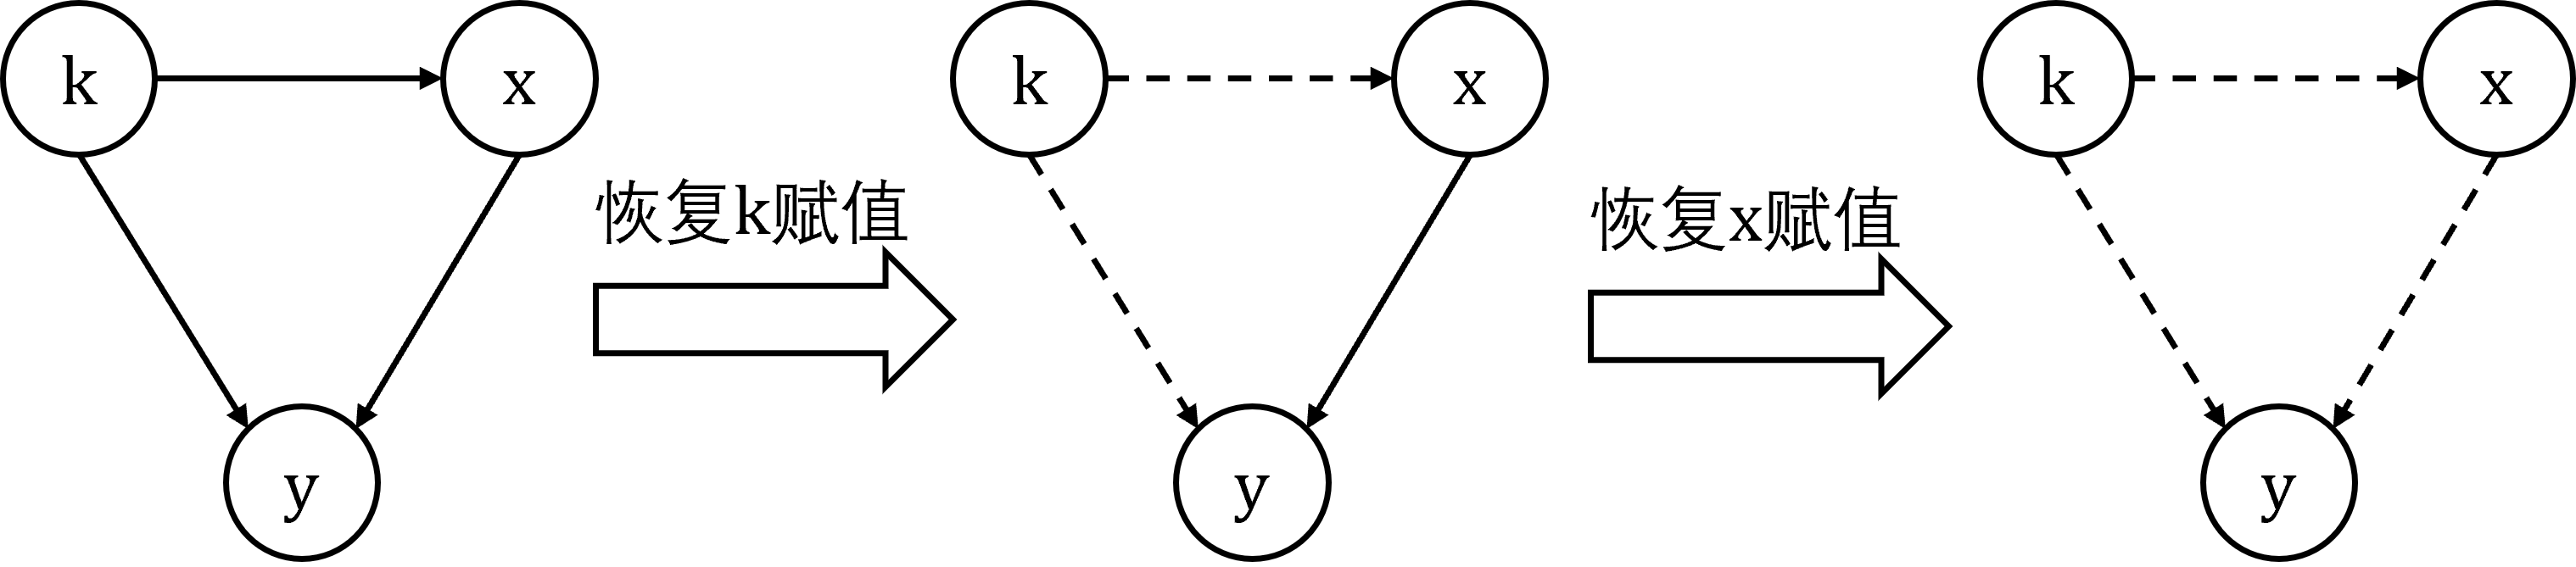
\includegraphics[width=\columnwidth]{Img/restore1.png}
    \bicaption {等式约束关系图。} {Demo of equality constraint graph.}
\label{fig:restore1}
\end{figure*}


\begin{example}
\label{ex:restore1}
假设当前近似解为$\{k \mapsto 1, x \mapsto 1, y \mapsto 1\}$,且有如下等式约束:$\{P_1: (k^2 + 3k) x + 6k = 0, P_2: k^2 x^2 + 3y = 0\}$。约束$P_1$和$P_2$可以分别关联变量$x$和$y$,我建立等式关系图如图\ref{fig:restore1}。
\begin{enumerate}
    \item 建立变量和等式约束关联:$x \sim P_1, y \sim P_2$
    \item 考虑当前节点的入度,变量$k$的入度为0,不被等式所限制,变量$x$的入度为1,受变量$k$的赋值直接影响,变量$y$的入度为2,受变量$x$和$k$的赋值直接影响。
    \item 从自由变量$k$开始考虑,消去起点为$k$的有向边,此时变量$x$的入度为0。
    \item 推断$x \mapsto -1.5$,赋值后消去起点为$x$的有向边。
    \item 此时变量$y$的入度为0,推断赋值为$y \mapsto -0.75$。
    \item 检查当前赋值$\{k \mapsto 1, x \mapsto -1.5, y \mapsto -0.75\}$满足所有约束。
\end{enumerate}
\end{example}


\subsection{第二种恢复方法:小范围局部搜索}
当第一种方法不能解决所有等式约束可满足状态时,我使用第二种方法进行恢复。第二种方法使用一种简化版本的局部搜索算法(limited local search)来尝试将近似解移动到最终的精确解。首先,我把所有松弛的约束恢复为起始状态,然后继续在算术变量上运行局部搜索,直到找到了一组精确解或者局部搜索没有改进为止。相比于主流程中的局部搜索,恢复阶段的局部搜索算法是一种局限的版本,因为我舍弃了布尔变量的迭代,以及一些随机步骤的发生。并且在实际运行中,近似解往往已经满足了绝大多数约束,因此受限版本的局部搜索算法只聚焦于几个尚且没有满足的等式约束,迭代的速度和运行效率要快很多。相比于第一种方法,第二种方法一般用于等式约束传播不为明显的情况,例\ref{ex:restore2}给出了一种情况。

\begin{example}
考虑逻辑公式$\Phi = x^2 + y^3 = 8 \wedge 2x^2 - 3y^2 > 6$,目前的近似解为$\{x \mapsto 12, y \mapsto -1.54\}$,仅满足松弛等式约束和不等式约束。恢复为原始状态后,等式约束不再满足,开始进行局部搜索。
\begin{itemize}
    \item 考虑针对原始等式约束固定变量$x$和$y$的两种关键移动,因为赋值复杂度的考量,选择操作$\{y \mapsto -\sqrt[3]{136}\}$
    \item 经过检查,赋值同时满足两个约束,找到精确解$\{x \mapsto 12, y \mapsto -\sqrt[3]{136}\}$。
\end{itemize}
\label{ex:restore2}
\end{example}

算法\ref{alg:relaxation}展示了加入了松弛机制后的局部搜索算法。和以往算法的主要区别在于,当一个变量的赋值复杂度超过了$\epsilon_v$时,等式约束会被松弛。当所有的约束都被满足时(找到了近似解),根据松弛约束的结构(第一种恢复方法)尝试找到附近的一个精确解。如果此方法失败,我尝试局限版本的局部搜索(第二种方法),直到找到一个精确解或者局部搜索没有改进为止。如果以上尝试均失败,尝试使用一种新的赋值方式重启。

\begin{figure*}[t]
    \centering
    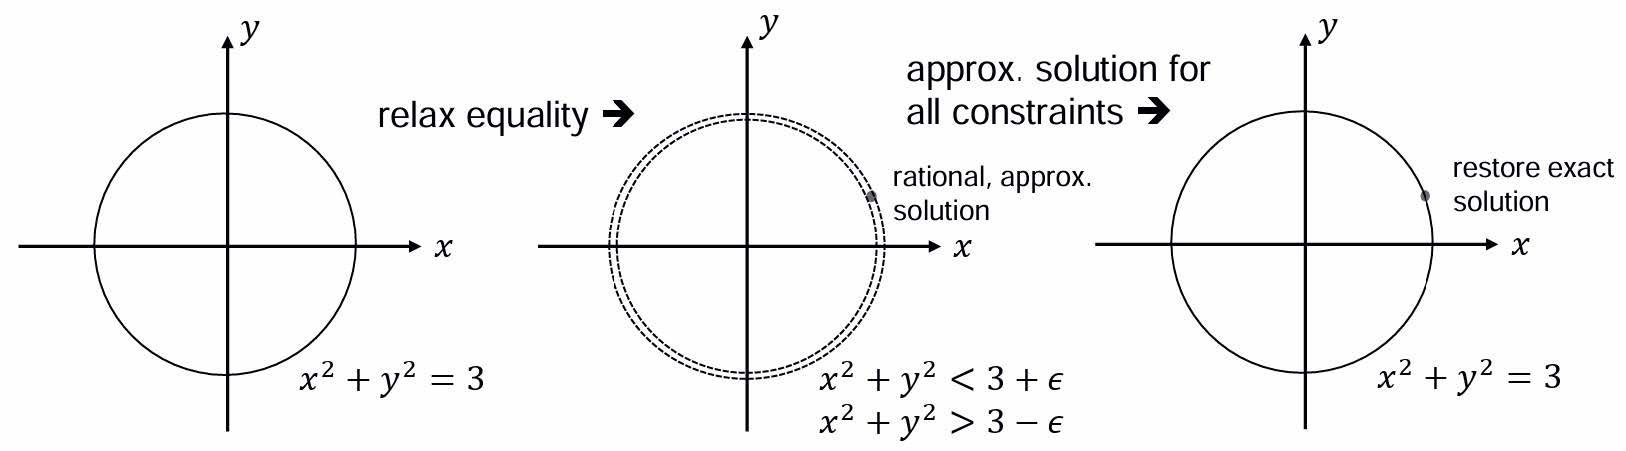
\includegraphics[width=\columnwidth]{Img/relax.jpg}
    \bicaption {等式松弛和恢复机制示意图。} {Demo of relaxation and restoration for equalitiy constraints.}
\label{fig:relaxation}
\end{figure*}

实际上,我在实验中发现两种寻找精确解的启发式方法在不同场景下有不同的用处。第一种基于等式约束结构的方法在涉及到线性方程时表现很好。第二章方法能够很好地处理变量存在多个赋值区域的情况,但是仍然很难保证同时满足所有的不等式约束。事实上,应用很多先进的方法来精确求解等式约束十分有前景\cite{CimattiGLS22, LiXZ23b}。但是,本文提出的方法仍然可以简单地拓展到更复杂的约束中,并且独立地验证精确解的存在。

\section{本章小结}
本章节主要讨论了LS\_NRA应对非线性实数算术特有的等式约束无理数赋值的解决策略。首先,本文回顾了以往工作中针对赋值复杂度的讨论,并进一步将这个概念拓展到代数数赋值上。然后,本文给出了等式松弛的概念,其原理是暂时扩大可行域来支持有理数赋值。最后,本文讨论了两种用于产生精确解的恢复算法,并讨论了两种算法的适用场景。

\begin{algorithm}[t]
    \caption{Relaxation of Equalities}
    \label{alg:relaxation}
    \textbf{Input}: A set of clauses $F$ \\
    \textbf{Output}: An assignment of variables that satisfy $F$, or failure
    
    \begin{algorithmic}[1] %[1] enables line numbers
        \Statex \hrulefill
        \STATE Initialize assignment to variables;
        \While {\top}
            \IF{all clauses satisfied}
            \STATE success \leftarrow find exact solution by analyzing structures;
            \IF{success}
            \RETURN success with assignment;
            \ELSE
            \STATE Restore relaxed constraints to original form;
            \STATE success \leftarrow limited local search;
            \IF{success}
            \RETURN success with assignment;
            \ELSE
            \STATE Perform major restart;
            \ENDIF
            \ENDIF
            \ENDIF

            \IF{time or step limit reached}
            \RETURN failure;
            \ENDIF

            \IF{no improvement for certain steps}
            \STATE Perform minor restart;
            \ENDIF
            
            \STATE Proceed algorithm as Algorithm \ref{alg:basic};
        \EndWhile

        \STATE \textbf{return} failure
    \end{algorithmic}
\end{algorithm}
\chapter{LS\_NRA的工具实现}\label{chap:implementation}

本章节主要介绍了LS\_NRA的整体框架和算法细节。除了前面两章介绍的胞腔跳跃缓存机制和等式松弛机制,我们还为非线性问题操作的停滞设计了简单的前瞻机制。然后,我们详细讨论本工具的具体实现,包括预处理阶段、重启策略、线性方程的快速运算、变量可行域的计算以及参数设置。

\section{启发式移动和前瞻机制}
如前文所述,非线性算数理论的一个挑战就是并不总是存在单变量的关键移动来满足一个特定的约束。之前的做法更多依赖于沿着固定直线的参数方程替代\cite{LiXZ23},更一般的做法需要用到柱形代数分解或多项式优化等理论。特别地,在SMT-LIB测试样例中,一类来自于生物网络\cite{AkutsuHT08}的名为Sturm-MBO的样例覆盖了大量的非常复杂的多项式,并且规定所有变量只能取正值。当多项式包含很多变量时,目前的启发式搜索方法很难找到满足约束的赋值。

本小节提出一种新的应对这种问题的方法,并且保证每次仍然只移动一个变量。为方便说明,我们首先定义文字的停滞状态如\ref{def:stuck}所示:

\begin{definition}{\textbf{停滞(Stuck)}}
    一个文字$l$被称为停滞,当且仅当$l$目前处于未满足状态,并且对于$l$中的任何一个变量$x$,都不存在一个关键移动$cm(l, x)$使其满足。
\label{def:stuck}
\end{definition}

以往工作\cite{LiXZ23}提出了一种多变量同时移动的关键移动操作,但是受限于直线的方向向量选择,在实际使用中多变量移动的效率较低。本文提出了一种新的启发式移动策略,通过多步前后移动来寻找满足约束的赋值。给定一个目前处于停滞状态的文字$l$,我们首先在$l$中选择一个系数(根据其他变量的赋值决定)不为0的变量$x$,然后启发式地选择一系列候选移动作为$x$接下来的赋值。对于每一个候选值来说,我们计算文字$l$在赋值后是否仍然处于停滞状态。我们优先选择那些没有处于停滞状态的候选赋值。

假定当前赋值$x_0$,变量$x$的可行域为$I$,启发式的移动选择包括以下几种:
\begin{itemize}
    \item 可行域$I$的每个区间中,靠近边界值的有理数和整数。有理数被设定为与边界值相差$10^{-4}$。比如,对于可行域$[11.2, 15.1]$,选择的移动有$\{11.2, 12, 15, 15.1\}$。
    \item 比$x_0$大于或小于的临近整数。比如,对于当前赋值$x_0 = 13.5$,选择的移动有$\{13, 14\}$。
    \item 从区间$[\frac{x_0}{2}, x_0)$中均匀地选取三个值,从区间$(x_0, 2x_0]$中均匀选取三个值。
\label{en:look-ahead}
\end{itemize}

第一类操作反映了变量$x$约束的信息。第二类操作借鉴了随机游走的思想,并且优先选择简单的整数值。第三种操作是最常见的,允许在更小或者更大的分数上进行搜索。算法\ref{alg:look-ahead}总结了以上的基本思想。我们用集合$S$收集候选赋值的移动,然后循环验证集合$S$中的每一个元素。如果文字$l$在赋值之后没有陷入停滞状态,那么返回这个赋值。否则,返回集合$S$中的随机元素。

我们以例\ref{ex:look-ahead}进行说明。

\begin{example}
如图\ref{fig:look-ahead}所示,考虑公式$F = \{(x - 2)^2 + (y - 2)^2 \leq 1\}$,当前赋值为$\alpha = \{x \mapsto 0.7, y \mapsto 0.7\}$,变量$x$和$y$的可行域都是$\emptyset$。根据启发式赋值\ref{en:look-ahead}第三条,我们可以选择一种候选赋值$x \mapsto 1.4$作为猜测,移动后变量$y$的可行域为$[1.2, 2.8]$,因此该前瞻赋值成功,本次迭代算法直接进行两次赋值。

\begin{figure*}[t]
    \centering
    
\includegraphics[width=0.7\columnwidth]{Img/look-ahead.png}
    \bicaption {前瞻策略示意图。} {Demo of look-ahead strategy.}
\label{fig:look-ahead}
\end{figure*}
\label{ex:look-ahead}
\end{example}

\begin{algorithm}[t]
    % \small
    \caption{Heuristic choice of candidate values and look-ahead for critical moves}
    \label{alg:look-ahead}
    \textbf{输入}: Literal $l$ that is stuck\\
    \textbf{输出}: Candidate variable $v$ and new value $x_1$
    
    \begin{algorithmic}[1] %[1] enables line numbers
        \Statex \hrulefill
        \STATE $x \leftarrow$ variable in polynomial  $l$ with non-zero coefficient;
        \STATE $S \leftarrow$ heuristic move selection for variable $x$;
        \FOR {value $x_1$ in $S$}
            \IF {$l$ has critical move after assigning $x$ to $x_1$}
                \RETURN $x, x1$;
            \ENDIF
        \ENDFOR
        \STATE $x_1 \leftarrow$ random chosen value in $S$;
        \STATE \RETURN $x, x_1$
    \end{algorithmic}
\end{algorithm}

\section{实现细节}
LS\_NRA主要在Z3定理证明器上实现,并且使用Z3原生的多项式和代数数库。我们的工具借鉴了Z3中MCSAT算法的实现,共享了文字、子句的数据结构,但是内部算法逻辑和代码实现完全独立。下面我们将主要介绍LS\_NRA的几个模块。整体工具框架如图\ref{fig:total}所示。

\begin{figure*}[]
    \centering
    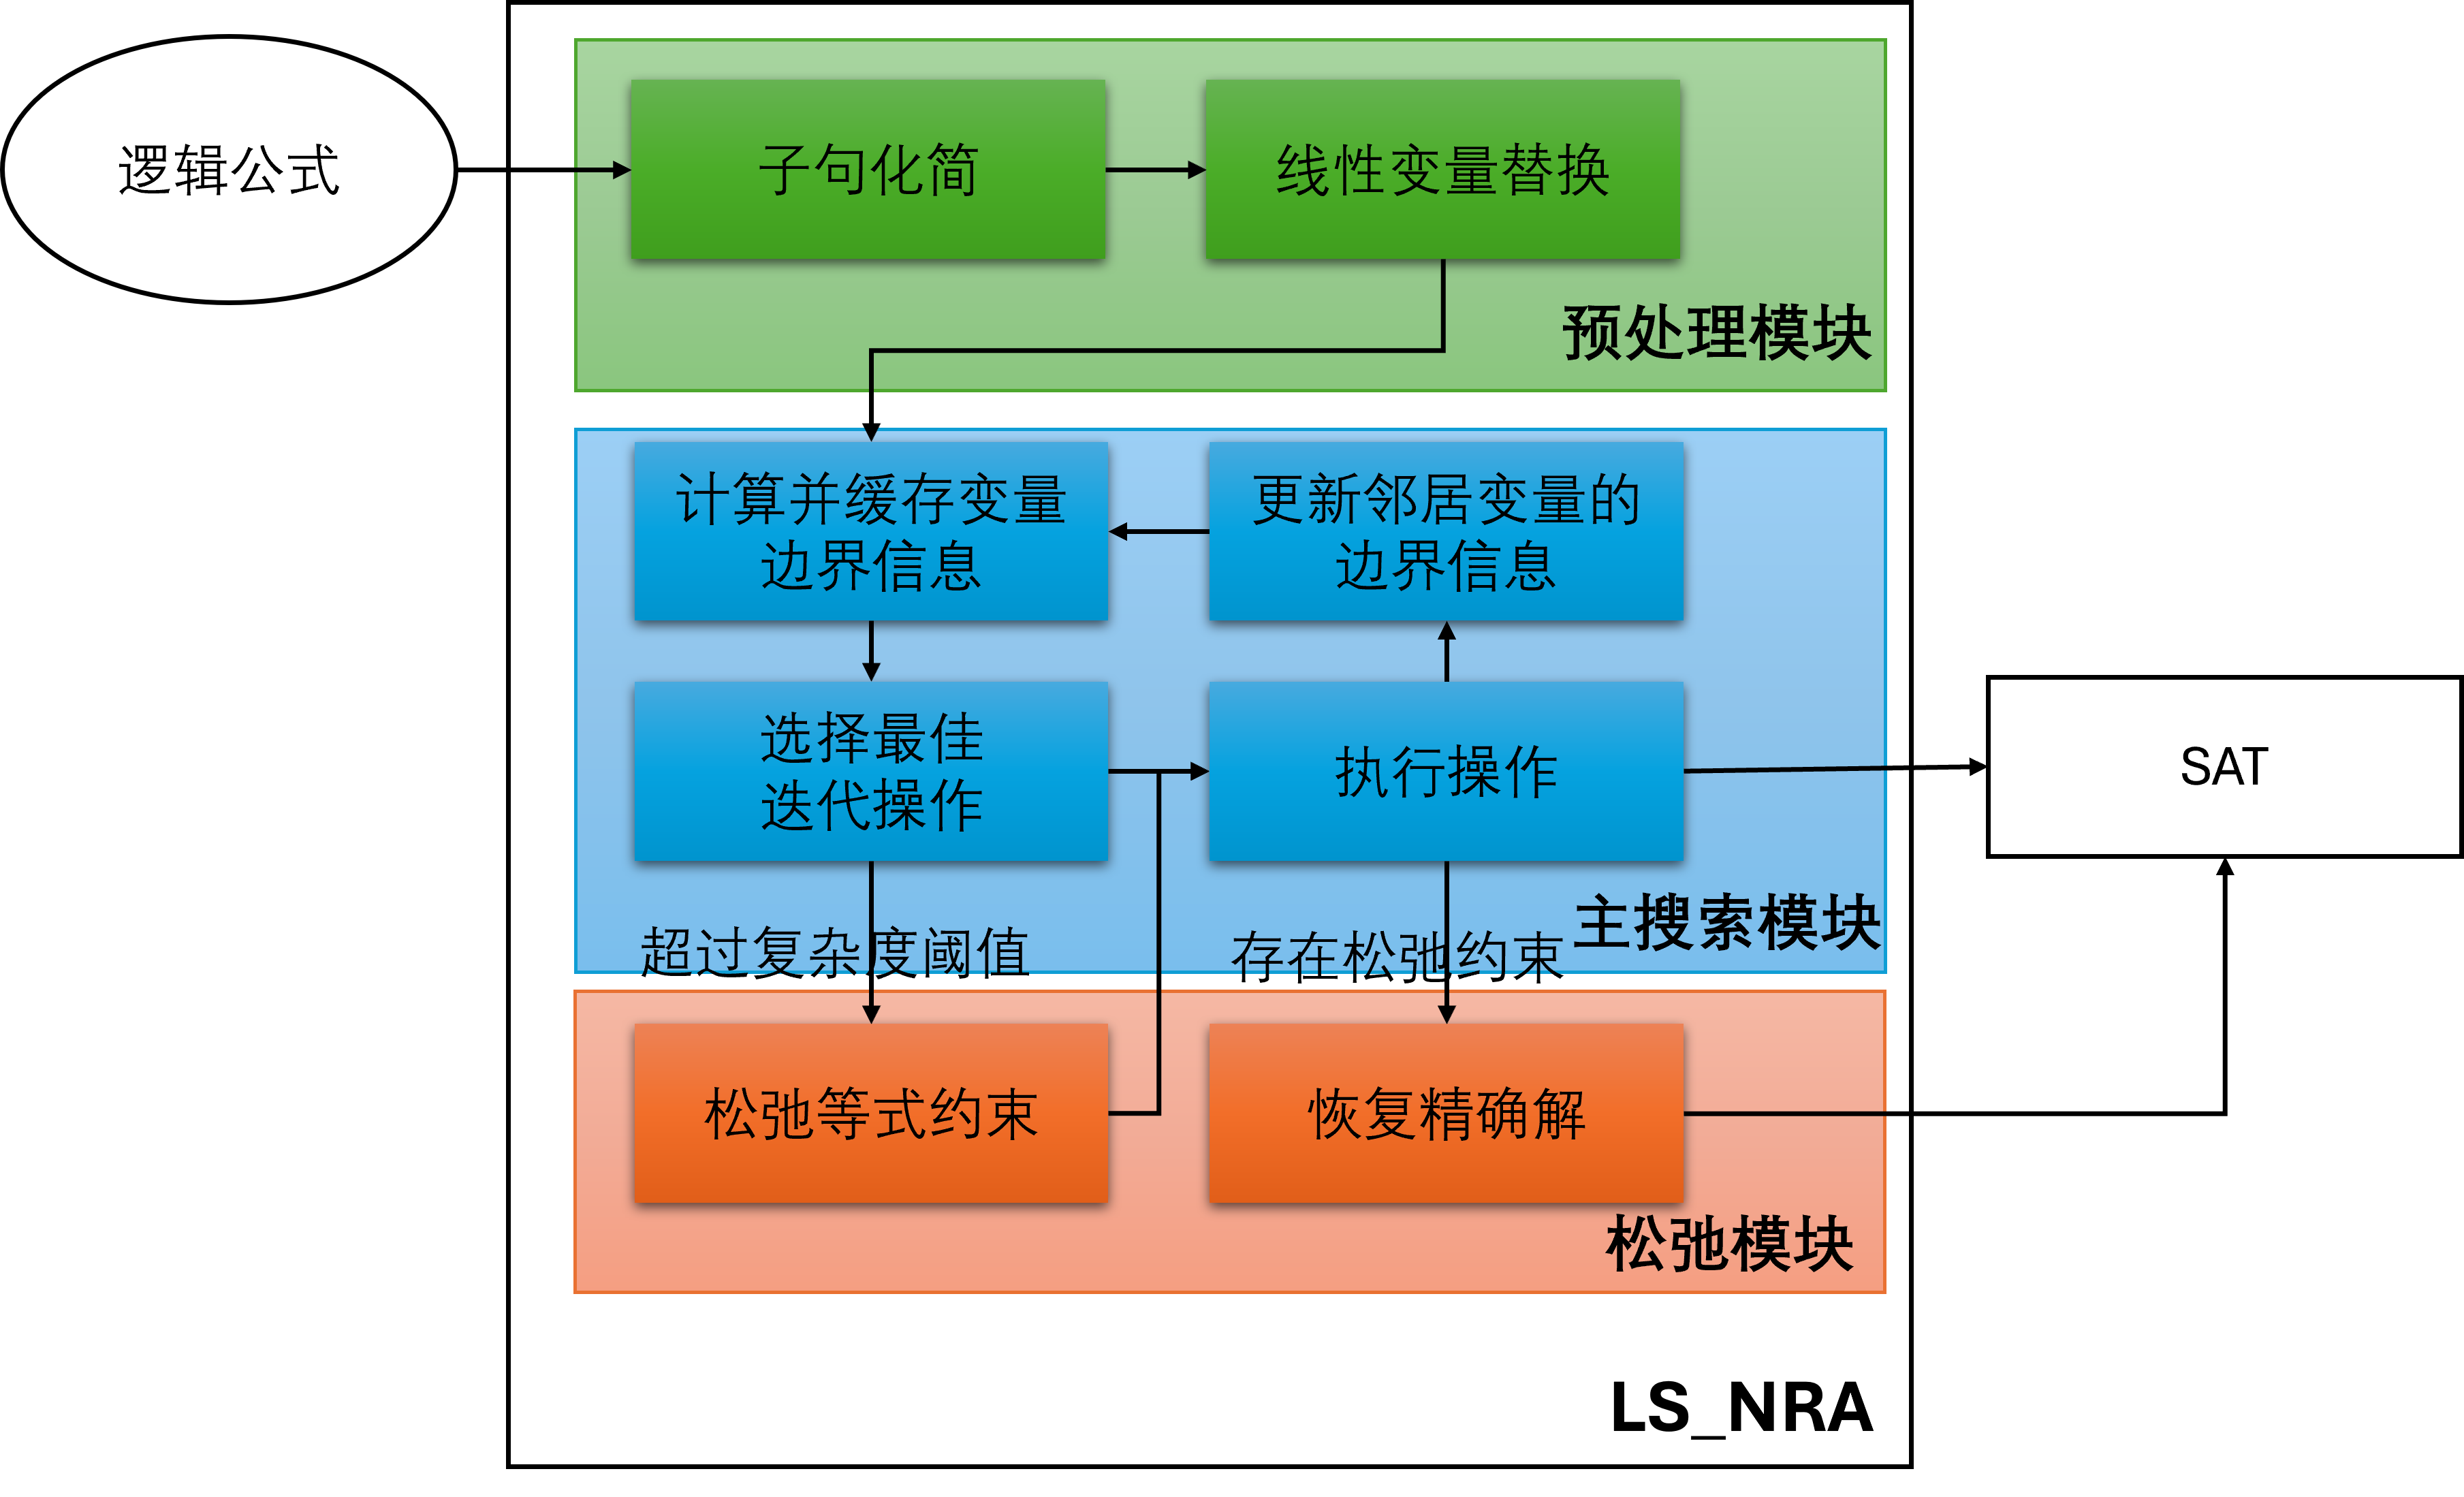
\includegraphics[width=0.9\columnwidth]{Img/structure.png}
    \bicaption {工具整体框架。} {Overall framework of LS\_NRA.}
    \label{fig:total}
\end{figure*}

\textbf{预处理阶段:} 预处理阶段主要负责化简主要的子句形式,以及简单的变量替换,为后续的主要搜索过程提供方便。
\begin{itemize}
    \item \textbf{子句化简:} 将同时出现的子句$p \le 0$和$p \ge 0$合并为$p = 0$。
    \item \textbf{变量替换:} 在形如$c \cdot x + q = 0$的等式约束中,其中$c$是常数,$q$是次数最多为1的多项式并且最多包含2个变量,替换掉变量$x$。这里我们限制$q$的形式以降低变量替换的复杂度。
\end{itemize}

\textbf{重启策略:} 我们设计了一个双层的重启策略,参数分别为$T_1$和$T_2$,值为100。其中一次\textbf{小重启}在$T_1$次迭代没有改进后执行,随机选择未满足子句中的一个变量修改赋值。在$T_2$次小重启之后,一次\textbf{大重启}会重置所有变量的赋值。

\textbf{加权策略:} 本工作引入PAWS(pure additive weighting scheme)\cite{PAWS}作为加权策略。PAWS的基本思想是初始为每个子句设置权重为1,所有为满足的子句在局部最优时权重加1,当子句权重增加一定次数后一次性减少所有子句的权重。目前主流的SAT求解器比如EagleUP\cite{eagleup}和Sparrow2011\cite{sparrow}都采用了这张技术。

\textbf{线性方程的快速运算:} 本文的实根隔离是基于Z3现有的多项式操作库完成的,其原理是牛顿迭代。但是当变量在多项式中以线性项出现时,我们可以通过斜率快速计算可行域,而非使用更通用的实根隔离函数。

\textbf{参数设置:} 本工作的可调参数设置如表\ref{tab:parameter}所示。

\begin{table*}[]
    \centering
    \resizebox{0.7\linewidth}{!}{
        \begin{tabular}{c | c | c}
            符号 & 参数说明 & 预设值 \\\hline
            $sp$ & PAWS加权策略的概率 & 0.006\\\hline
            $T_1$ & 小重启执行所需的无提升迭代次数 & 100\\\hline
            $T_2$ & 大重启执行所需的小重启次数 & 100\\\hline
            $\epsilon_v$ & 等式松弛所需的复杂度阈值 & $10^{-4}$\\\hline
            $\epsilon_c$ & 等式松弛的程度 & $10^{-4}$\\\hline
        \end{tabular}
        }
        \bicaption{算法的可调参数设置。} {Tunable parameters of the algorithm.}
\label{tab:parameter}
\end{table*}

\section{本章小结}
本章节主要讨论了LS\_NRA的实现细节,包括启发式移动和前瞻机制、预处理阶段、重启策略、线性方程的快速运算以及参数设置。具体来说,我们给出了局部搜索算法中常见的停滞状态,然后给出了一种启发式候选赋值策略。接着,我们针对每个不同的环节给出了快速运算的策略,并且描绘了整体的结构示意图。

\chapter{实验设计及结果分析}\label{chap:Result}

本章节主要介绍基于前述算法设计的LS\_NRA求解工具的实验结果,并基于此对其性能进行了分析。本章节主要可以分为三个部分:首先我们介绍实验安排和实验条件,包括测试样例、比较方法、运行环境等;然后我们给出LS\_NRA与其他主流求解器的求解个数与时间对比;最后我们对前几章提出的策略设计了消融实验,确保本文介绍的算法的有效性。

\section{实验设置}
\subsection{测试样例}
本工作选取SMT-LIB\footnote{\url{https://smt-lib.org/}}中QF\_NRA理论作为测试样例。测试样例大多包含来自工业问题的实例,我们介绍其中一些类别如下:

\begin{itemize}
    \item \textbf{2019-ezsmt:} 该类别来自一种处理non-tight程序的工具EZSMT+。
    \item \textbf{20170501-Heizmann:} 该类别来自Ultimate程序分析框架的一个组件,主要用于基于约束的不变式合成。
    \item \textbf{20200911-Pine:} 该类别来自名为Pine的工具,主要用于检查循环不变式的归纳性。
    \item \textbf{LassoRanker:}该类别来自一种使用秩函数来分析Lassoshaped程序终止性的工具,所含样例都是多线性(multilinear)约束。
    \item \textbf{UltimateAutomizer:}该类别产生自基于自动机的软件模型检查工具,是Ultimate软件分析工具的一个组件。
\end{itemize}

\textbf{样例选择:} 在SMT-LIB中,每一个测试样例会标注标签(label),即SAT、UNSAT或UNKNOWN,用来表示是否被其他的求解器求解。由于局部搜索算法只能用来求解可满足的样例,因此我们首先使用主流的SMT求解器(Z3、cvc5、Yices)来被证明为UNSAT的样例,最终留下潜在的可满足样例作为本文的最终测试样例。最终我们收集了6216个测试样例。


\subsection{实验方法}
 \textbf{实验环境:} 所有实验都在一台配备有Intel Xeon Platinum 8153(2.00GHz)和2048G RAM 的服务器上进行,系统为Centos 7.7.1908。每一个样例设置的时间限制为20分钟(和SMT比赛相同),内存限制为30GB。由于我们的工具LS\_NRA实在Z3上实现的,我们保留了默认的随机数设置,来确保与原版Z3求解器对比的公平性。

\textbf{比较方法:} 对于每一个样例,求解器可以输出求解结果(SAT、UNSAT或TIMEOUT)、运行时间和内存占用等信息。我们收集每一个求解器的信息用于后面的结果展示。除此之外,我们对主流求解器均采用默认设置,比如默认不采用增量式求解,全部使用串行方法等。

\section{LS\_NRA求解NRA样例的能力}
我们在表\ref{tab:experiment}中展示了我们的工具LS\_NRA与其他主流SMT求解器的性能对比。我们的工具一个主要优势是针对Sturm-MBO样例,一种只包含一个非常复杂度数很高的多项式的约束。目前主流的完备算法在该问题上没有求解成功。我们的工具在其他样例上表现也很突出,基本可以和主流求解器的效果持平。

除此之外,我们的算法和Z3、cvc5有很大的互补性。根据表\ref{tab:experiment},一共有来自不同类别共148个样例仅仅可以使用局部搜索算法求解,而非Z3、cvc5、Yices等完备算法。更具体来说,有291个样例可以被局部搜索求解而非Z3,有378个样例可以被局部搜索求解而非cvc5。

\begin{table*}[]
    \centering
    \resizebox{0.9\linewidth}{!}{
        \begin{tabular}{c | c | c | c | c | c | c}
            \hline
            类别 & 个数 & Z3 & cvc5 & Yices & LS\_NRA (本文) & 单独求解 \\\hline
            20161105-Sturm-MBO & 120 & 0 & 0 & 0 & 84 & 84 \\
            20161105-Sturm-MGC & 2 & 2 & 0 & 0 & 0 & 0 \\
            20170501-Heizmann & 60 & 2 & 1 & 0 & 6 & 5 \\
            20180501-Economics-Mulligan & 93 & 93 & 89 & 91 & 87 & 0 \\
            2019-ezsmt & 61 & 56 & 50 & 52 & 18 & 0 \\
            20209011-Pine & 237 & 234 & 199 & 235 & 224 & 0 \\
            20211101-Geogebra & 112 & 110 & 91 & 99 & 100 & 0 \\
            20220314-Uncu & 74 & 69 & 62 & 70 & 70 & 0 \\
            LassoRanker & 351 & 167 & 305 & 122 & 284 & 15 \\
            UltimateAtomizer & 48 & 35 & 35 & 39 & 26 & 2 \\
            hycomp & 492 & 307 & 225 & 227 & 270 & 17 \\
            kissing & 42 & 33 & 17 & 10 & 33 & 2 \\
            meti-tarski & 4391 & 4391 & 4343 & 4369 & 4356 & 0 \\
            zankl & 133 & 70 & 58 & 58 & 99 & 26 \\\hline
            总和 & 6216 & 5569 & 5475 & 5372 & 5657 & 151 \\\hline
        \end{tabular}
        }
        \bicaption{LS\_NRA和其他SMT求解器的求解能力对比。} {Comparison of LS\_NRA and other SMT solvers.}
\label{tab:experiment}
\end{table*}

我们在图\ref{fig:scatter}中描绘了LS\_NRA与Z3、cvc5、Yices求解时间对比的散点图。图中每一个点的横坐标代表了求解该样例LS\_NRA所需要的时间,纵坐标表示了其他求解器的求解时间,虚线则说明二者在该问题上消耗的求解时间一致。我们注意到在SMT-LIB测试样例中存在大量相对简单的问题。为了考虑这些问题的因素,我们统计了Z3、cvc5和LS\_NRA在1秒内解决的问题个数,共计4765个,这样仅仅剩下1451个被认为是难以求解的样例。从这点来看,LS\_NRA在求解总数、单独求解和互补性上均有优势。

\begin{figure*}[t]
    \centering
    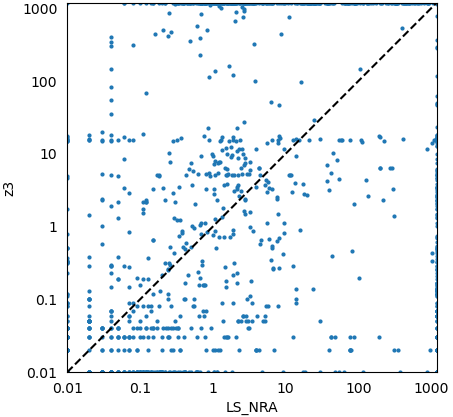
\includegraphics[width=0.25\columnwidth]{Img/scatter_z3.png}\qquad
    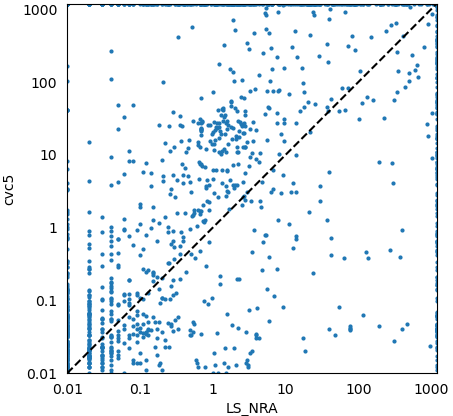
\includegraphics[width=0.25\columnwidth]{Img/scatter_cvc5.png}\qquad
    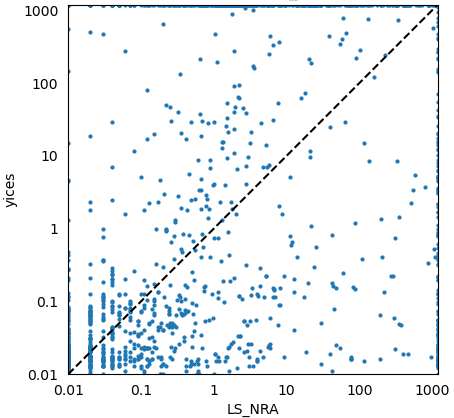
\includegraphics[width=0.25\columnwidth]{Img/scatter_yices.png}
    \bicaption{LS\_NRA与Z3、cvc5、Yices求解时间对比。} {Comparison of LS\_NRA and Z3, cvc5, and Yices solving time.}
\label{fig:scatter}
\end{figure*}

我们还参考了不同求解器的求解时间对比,如图\ref{fig:time}所示。可以看出,几乎在任何的限制时间内,局部搜索算法的求解数量都是最多的,这说明了局部搜索的相对轻捷。随着求解时间的增加,局部搜索算法的求解数量增长速度远远快于其他求解器,这说明在充足的时间内,更多的样例可以通过多次迭代找到邻近的可行解。
\begin{figure*}[t]
    \centering
    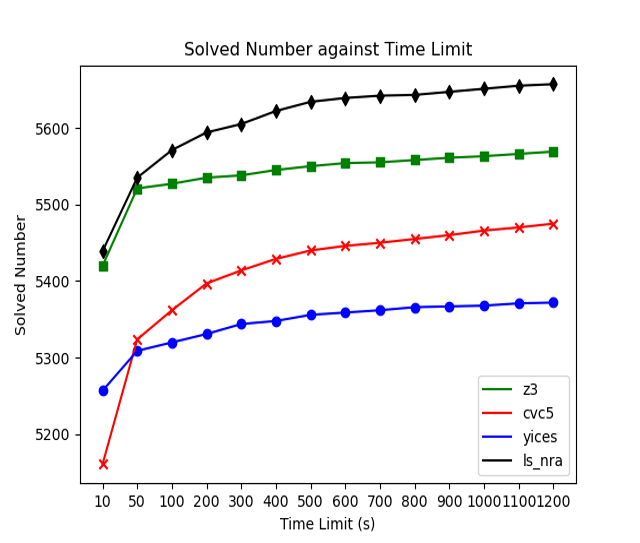
\includegraphics[width=0.7\columnwidth]{Img/time_solver.png}
    \bicaption{LS\_NRA与Z3、cvc5在不同时间求解个数对比。}{Comparison of LS\_NRA and Z3, cvc5 solving number in different time.}
\label{fig:time}
\end{figure*}


\section{和其他局部搜索工作的对比}
我们还讨论了LS\_NRA与以往局部搜索工作的对比。在\cite{multilinear}考虑的979个多线性样例中,LS\_NRA可以求解826个,略小于前序工作的891个。这种微弱的差异主要来自于\cite{multilinear}更高效的实现,考虑到其工作进需要考虑有理数赋值,而非代数数,因此在数据结构设计和参数优化上更有针对性。在\cite{LiXZ23}考虑的2736个样例中,我们的方法可以求解2589个,高于前序工作的2246个。事实上,我们不仅比局部搜索算法求解的个数要多,也要比前面工作用于对比的其他求解器个数还要多。我们注意到\cite{LiXZ23}使用了不同的计算软件(比如Maple),并且在不同机器上测试,因此数据可能略有误差。

\section{消融实验1:变量分数增量式计算的影响}
本小节主要展示章节\ref{chap:method1}中提出的变量分数增量式计算对迭代加速的影响。我们比较如下集中实现:基于边界的增量式计算(Incremental),不采用增量式计算的传统方法(Naive),以及传统方法但是限制每次考虑的子句数最大为45(Limit-45)。相关的结果如表格\ref{tab:incremental}所示。

我们注意到不同实现方法的求解总数差异并不大,并且主要集中在LassoRanker类别上。LassoRanker样例一般需要比较长时间求解,因此不同实现方法对迭代速度的影响十分重要。通过对比求解时间可以看出对于一个特定的问题而言,Naive和Limit-45的方法基本需要消耗2-10倍于Incremental方法的时间,具体的倍数在不同问题上有所不同。

图\ref{fig:time_inc}显示了是否使用增量式计算在不同时间限制下的求解个数。对于1200秒的限制来说,是否使用增量式计算对求解个数的影响并不明显,但是在更少的求解时间时(300秒以下),更多的计算资源消耗在了实根隔离和可行域计算上,因此在迭代中缓存这些昂贵的信息尤为重要。在求解时间为10秒的条件下,二者的差距有150个以上,这说明了增量式计算对于提升求解速度的重要性。

\begin{figure*}[t]
    \centering
    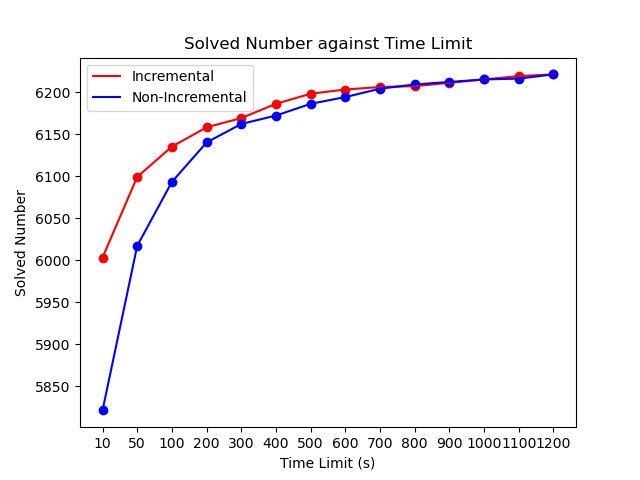
\includegraphics[width=0.7\columnwidth]{Img/time_inc.png}
    \bicaption{LS\_NRA使用增量式计算在不同时间下求解的个数。}{Number of solutions found by LS\_NRA with incremental calculation in different time.}
\label{fig:time_inc}
\end{figure*}

\begin{table*}[]
    \centering
    \resizebox{0.8\linewidth}{!}{
        \begin{tabular}{c | c | c | c | c}
            \hline
            类别 & 个数 & Incremental & Naive & Limit-45 \\\hline
            20161105-Sturm-MBO & 120 & 84 & 84 & 84 \\\hline
            20161105-Sturm-MGC & 2 & 0 & 0 & 0 \\\hline
            20170501-Heizmann & 60 & 6 & 5 & 5 \\\hline
            20180501-Economics-Mulligan & 93 & 87 & 88 & 88 \\\hline
            2019-ezsmt & 61 & 18 & 19 & 15 \\\hline
            20209011-Pine & 237 & 224 & 221 & 221 \\\hline
            20211101-Geogebra & 112 & 100 & 99 & 99 \\\hline
            20220314-Uncu & 74 & 70 & 70 & 70 \\\hline
            LassoRanker & 351 & 284 & 262 & 267 \\\hline
            UltimateAtomizer & 48 & 26 & 26 & 26 \\\hline
            hycomp & 492 & 270 & 257 & 257 \\\hline
            kissing & 42 & 33 & 32 & 33 \\\hline
            meti-tarski & 4391 & 4356 & 4345 & 4345 \\\hline
            zankl & 133 & 99 & 98 & 98 \\\hline
            总和 & 6216 & 5657 & 5606 & 5608 \\\hline
        \end{tabular}
        }
        \bicaption{增量式计算对算法的影响。} {Impact of incremental calculation on algorithm.}
\label{tab:incremental}
\end{table*}

\section{消融实验2:等式约束松弛的影响}
本小节主要展示章节\ref{chap:method2}中介绍的等式约束松弛对整体算法的影响。我们给出以下三种版本:使用等式松弛机制(Relaxation),不适用等式松弛但优先选取低复杂度的赋值(Threshold),不使用等式松弛并且不考虑赋值复杂度(NoOrder)。相关结果在表\ref{tab:relaxation}中展示。

试验结果表明,当把赋值复杂度考虑在内时可以保证对于大多数类别提升求解能力。

\begin{table*}[]
    \centering
    \resizebox{0.8\linewidth}{!}{
        \begin{tabular}{c | c | c | c | c}
            \hline
            类别 & 个数 & Relaxation & Threshold & NoOrder \\\hline
            20161105-Sturm-MBO & 120 & 84 & 85 & 84 \\\hline
            20161105-Sturm-MGC & 2 & 0 & 0 & 0 \\\hline
            20170501-Heizmann & 60 & 6 & 9 & 3 \\\hline
            20180501-Economics-Mulligan & 93 & 87 & 89 & 86 \\\hline
            2019-ezsmt & 61 & 18 & 18 & 18 \\\hline
            20209011-Pine & 237 & 224 & 220 & 220 \\\hline
            20211101-Geogebra & 112 & 100 & 100 & 92 \\\hline
            20220314-Uncu & 74 & 70 & 70 & 70 \\\hline
            LassoRanker & 351 & 284 & 283 & 278 \\\hline
            UltimateAtomizer & 48 & 26 & 24 & 19 \\\hline
            hycomp & 492 & 270 & 204 & 158 \\\hline
            kissing & 42 & 33 & 31 & 27 \\\hline
            meti-tarski & 4391 & 4356 & 4348 & 4355 \\\hline
            zankl & 133 & 99 & 99 & 99 \\\hline
            总和 & 6216 & 5657 & 5580 & 5669 \\\hline
        \end{tabular}
        } 
        \bicaption{等式约束松弛对算法的影响。} {Impact of relaxation on algorithm.}
\label{tab:relaxation}
\end{table*}

\section{本章小结}
本章节通过设计实验,深入评估了LS\_NRA工具的求解性能和策略有效性。首先,我们对比了LS\_NRA和其他主流SMT求解器(Z3、cvc5、Yices)在SMT-LIB上的求解个数和求解时间,方法表明LS\_NRA对于高次约束具有优势。然后,我们设计消融实验测试了基于边界的可行域缓存机制和等式松弛机制对整体求解效果的影响,实验表明二者均对算法的求解能力有所提升。
\chapter{总结与展望}\label{chap:conclusion}

本章节主要对前面提出的创新点和工具实现进行系统的总结,归纳本工作主要的贡献,并讨论后续工作的可行性。

\section{工作总结}
SMT问题一直是形式化验证与软件工程领域的核心问题,SMT求解器在很多方面有着广泛的应用,很多验证算法最终都需要SMT求解器给出解答。非线性实数理论因为其约束的复杂性和无理数赋值的困难性,一直是SMT问题中的难点。以往的工作既有根据多项式胞腔理论设计的系统方法,也有从SAT问题借鉴而来的启发式方法,但是这些方法在实际应用中都有一定的局限性,在特定问题上表现不佳。本工作提出了一种针对非线性实数所有样例的局部搜索算法工具LS\_NRA。具体来说,其包含以下几部分组成:基于边界的胞腔跳跃分数缓存机制、等式约束松弛机制、非单变量操作的前瞻机制。实验表明,LS\_NRA在大多数情况下都能够在较短时间内找到解,并且相比于主流SMT求解器(Z3、CVC5)在高次约束上优势明显。

以往工作提出了用于算术理论的关键移动操作,针对非线性问题拓展成了胞腔跳跃操作。但是以往的工作只是针对单一子句而言,并没有基于变量级别的可行域来分析,造成了操作的冗余和迭代的低效。本工作首先提出了边界数据结构来模拟胞腔之间的间隔,基于此提出一种变量分数的增量式计算方法,而非传统的迭代计算,并且给出了边界信息的迭代条件和迭代信息,从而使得局部搜索单词计算量的下降和迭代性能的提升。

本工作的另一个创新点是针对等式约束的特殊处理。非线性实数理论是唯一一个涉及到无理数赋值的算术理论,这也是以往的局部搜索工作避开高次非线性约束的一个理由。本工作首先引入了赋值复杂度的概念,给出了赋值对迭代次数影响的分析,进而提出等式松弛机制,以暂时扩大可行域来增加赋值的可能性,从而提高了算法的求解能力。本工作还给出了两种恢复方法,即基于约束结构的传播机制和受限局部搜索,最终完成SMT问题精确解的搜索。

此外,本工作还探讨了实现细节。比如,本工作定义了无单变量操作的文字状态,并给出一种两种变量前后移动的前瞻机制,可以确保在给定的候选赋值中增加变量跳出停滞状态的可行性。此外,本工作还引入了两种重启机制,即单一变量或所有变量的重新赋值方法,并规定在一定步数迭代没有效果时使用。最后,本工作详细阐述了LS\_NRA的不同实现组件,包括预处理部分、线性方程的快速计算和参数的选择。

基于上述思想,本工作测试了LS\_NRA在同一测试环境下与其他局部搜索算法和主流SMT求解器的求解能力。实验表明,LS\_NRA整体上要优于其他主流方法,并且在高次约束上表现最优。经过消融实验,本文证明了以上方法的有效性,并且给出了每个组件的重要性。

\section{未来展望}
\subsection{局部搜索算法的拓展}
本工作作为局部搜索算法在算术理论的拓展,对后面的工作有很多启发作用。首先,目前的缓存机制仍然是基于边界数据结构的单变量可行域执行的,但是在实际的解空间$R^n$中,同一胞腔内每个变量的可行域都是固定的,因此更好的解决方法是能够定位到当前遍历的胞腔序号,这样可以确保重复遍历带来的可行域重复计算问题。其次,目前对于等式约束的松弛算法很基础,复杂度阈值是一个预设的常数,但是在实际搜索过程中应该区别不同难度的等式约束,即为不同难度的等式约束设置不同等级的阈值条件。再者,前序工作的多变量移动机制涉及到参数方程的方向向量选定问题,目前的工作都是基于预设的几组方向向量,而非动态调整。一个启发式的创新是使用强化学习方法实时检测不同方向对搜索状态的作用,然后实时调整多变量的搜索方向。

\subsection{更一般的约束形式}
本工作虽然是在多项式理论上完成的,但求解可行域与移动赋值的基本思想可以拓展到更一般的约束形式上。工作\cite{Trig}将局部搜索算法拓展到了三角函数上,区别在于求解可行域的方法不同。未来的一个可行工作是拓展到更复杂的函数上,比如神经网络的激活函数或分段函数等。局部搜索算法在高次约束上的求解能力也能够更好地应对高次约束的复杂性,从而在短时间内采样到可行解。

\subsection{与完备算法的互补}
如章节\ref{chap:Result}所述,局部搜索算法往往在高次约束上表现甚好,而完备算法则在强推理性的样例上表现突出。工作\cite{CaiZ21,hybridSMT,BoostMcsat}分别提出了用于SAT和SMT问题的混合求解方法,目前已经成为SAT-COMP和SMT-COMP的主流求解方法。一个预想的后续工作是将本文的边界数据结构纳入到完备算法中,即将局部搜索算法缓存的可行域机制应用到CDCL(T)/MCSAT算法上,来指导学习更有效的子句,从而减少整体求解遇到的冲突次数。

%---------------------------------------------------------------------------%
% main content
%-
%-> Appendix
%-
\cleardoublepage%
\appendix% initialize the environment
% \chapter{定理2.1的证明}

% appendix content
%-
%-> Backmatter: bibliography, glossary, index
%-
\backmatter% initialize the environment
\intotoc*{\cleardoublepage}{\bibname}% add link to toc
\artxifstreq{\artxbib}{bibtex}{% enable bibtex
    \bibliography{Biblio/ref}% bibliography
}{%
    \printbibliography% bibliography
}
%---------------------------------------------------------------------------%
%->> Backmatter
%---------------------------------------------------------------------------%
\chapter[致谢]{致\quad 谢}\chaptermark{致\quad 谢}% syntax: \chapter[目录]{标题}\chaptermark{页眉}
%\thispagestyle{noheaderstyle}% 如果需要移除当前页的页眉
%\pagestyle{noheaderstyle}% 如果需要移除整章的页眉

几年的硕士生涯走到了最后,值此论文完成之际,谨向求学路上所有给予我指导、支持与陪伴的师长、亲友致以最诚挚的感谢。

首先,我要对帮助过我的各位老师表达深深的感谢,包括曾经的导师詹博华副研究员、现任导师张立军研究员。他们作为我的导师帮助我初步拟定了课题的选定、基本的研究路线,并且帮助我养成了研究生该有的成熟心态。除此之外,蔡少伟老师作为约束求解领域的专家也对我的研究给出了十分宝贵的指导意见,吴志林老师也曾在整个毕业流程中多次对我施以援手。软件所的其余导师都无形之中或多或少对我给予了专业上的帮助和指引,他们的言传身教将是我未来学术道路上的重要财富。

其次,我也要向国重实验室的各位兄弟姐妹表达感谢。作为中途换过导师的学生,我曾经流转过多个课题组,他们在很多方面都给予了我极大的帮助。詹博华老师的学生帮助我很好地熟悉了学校的环境和基本的研究思路,蔡少伟老师的学生则更多在算法设计和具体的课题指引上担任起了领路人的帮助,张立军老师的学生则在最后一学年给予了我很多就业和未来发展的关键意见。可以说,国重实验室是一个充满了爱和帮助的大家庭,我很荣幸能够成为其中的一员。

再者,我也要感谢很多形式化社区的学者和从业人员。比如,我的工作更多是基于现有的SMT求解器开发的,因此Z3和cvc5等主要软件的开发团队是我的技术前辈,他们是使我看得更远的巨人,也是我永远要学习的楷模。我在英国参加VMCAI会议时,曾和来自不同国家、不同研究背景的同龄人热烈讨论过,他们对我的意见和对我工作的欣赏是我莫大的欣慰。我也要感谢国内的形式化社区,比如中国计算机学会的形式化方法专委会,他们为我提供了很多关于形式化方法的学习资源和交流机会。当然,我最应该感谢的其实还是投稿VMCAI会议时的无名审稿人,他们的审稿意见让我更好地打磨了自己的作品,让我欣慰地交上了这份答卷。功利地说,如果不是他们最后给出了正面的审稿意见,可能我的论文还未发表,我也未能顺利毕业。

未来,我可能会从事不同的行业和研究方向,但是硕士期间积累的宝贵经历是我人生地巨大财富。


\chapter{作者简历及攻读学位期间发表的学术论文与研究成果}

\section*{作者简历:}

王忠汉,男,辽宁大连人,1999年生,中国科学院软件研究所硕士研究生。

2017年9月——2021年6月,在南开大学电子信息与光学工程学院获得学士学位。

2021年9月——2025年6月,在中国科学院软件研究所攻读硕士学位。

\section*{已发表(或正式接受)的学术论文(加星号的表示共一作者):}

{
\setlist[enumerate]{}% restore default behavior
\begin{enumerate}[nosep]
    \item \textbf{Zhonghan Wang}, Bohua Zhan, Bohan Li, Shaowei Cai. Efficient Local Search for Nonlinear Real Arithmetic. (VMCAI 2024)
\end{enumerate}
}

% \section*{投稿经历}

% {
% \setlist[enumerate]{}% restore default behavior
% \begin{enumerate}[nosep]
%     \item AllDiff-LS: Solving Alldifferent Constraints with Efficient Local Search, AAAI 2023 过第一阶段,未中。
% \end{enumerate}
% }

\section*{参加的研究项目及获奖情况:}

\begin{enumerate}
    \item 参与了课题组可满足性模理论求解工具的工具开发和测试。
    \item 参与了课题组交互式定理证明的讨论。
\end{enumerate}

\cleardoublepage[plain]% 让文档总是结束于偶数页,可根据需要设定页眉页脚样式,如 [noheaderstyle]
%---------------------------------------------------------------------------%
% other information
\end{document}
%---------------------------------------------------------------------------%

